\documentclass{report}

\def \myTitle{\MakeUppercase{The Lost Expedition of \theIsland}} % workaround - \@title not always works...
\def \subtitle{Short Fan-made Adventure in \cosmereRPG}
\title{\myTitle{}}

\author{Pether.pg}

\usepackage[a4paper, total={7in, 9in}]{geometry}
\usepackage[dvipsnames]{xcolor}
\usepackage{xcolor}
\usepackage{ifthen}
\usepackage{changepage} % margins and adjustwidth 
\usepackage{graphicx} % insert images
\usepackage{pdfpages} % insert pdfs
\usepackage{ulem} % strikethrough \sout
\usepackage{multicol} % multicol
\usepackage{eso-pic} % for background images
\usepackage[absolute,overlay]{textpos} % to set possition of the box \begin{textblock*}
\usepackage{tikz} % for talent tree graphs
%\usepackage{emerald} % for hand-written ECFAugie
%\usepackage[T1]{fontenc} % for hand-written ECFAugie
\usepackage{caption} % for \captionsetup
\usepackage{titlesec}	% change how chapters are printed

\setlength{\columnsep}{20pt} % space between text columns


\usepackage{hyperref}
\hypersetup{colorlinks,citecolor=black,filecolor=black,linkcolor=black,urlcolor=black}

\usepackage{fancyhdr} % for fancy page numbering
\usepackage{nameref} % for \nameref{label}
\usepackage{cleveref}

\begin{document}
	
	
\definecolor{goldStats}{RGB}{208, 164, 82}
\definecolor{yellowQuote}{RGB}{245, 236, 221}
\definecolor{yellowRoleplay}{RGB}{244, 239, 233}
\definecolor{grayReason}{RGB}{200, 200, 200}
\definecolor{blueRadiance}{RGB}{30, 60, 96}
\definecolor{redSpoiler}{RGB}{200, 0, 0}

\newcommand{\linksBlack}{\hypersetup{colorlinks,citecolor=black,filecolor=black,linkcolor=black,urlcolor=black}}
\newcommand{\linksBlue}{\hypersetup{colorlinks,citecolor=blueRadiance,filecolor=blueRadiance,linkcolor=blueRadiance,urlcolor=blueRadiance}}

% \usepackage{titlesec}	% change how chapters are printed

\titleformat{\chapter}
	{\LARGE\bfseries\sffamily\color{blueRadiance}}
	{}
	{0em}
	{\linksBlue}
	[\linksBlack]
\titleformat{\section}
	{\Large\bfseries\sffamily\color{blueRadiance}}
	{\thesection}
	{1em}
	{\linksBlue}
	[\color{goldStats}\titlerule\linksBlack]
\titleformat{\subsection}
	{\large\bfseries\sffamily\color{blueRadiance}}
	{\thesubsection}
	{1em}
	{\linksBlue}
	[\linksBlack]
\titleformat{\subsubsection}
	{\bfseries\sffamily}
	{\thesubsection}
	{1em}
	{\linksBlue\color{blueRadiance}}
	[\linksBlack]
	
% \usepackage{fancyhdr} % for fancy page numbering
\fancyhf{} % Clear defaults
\newcommand{\defaultPageNumberStyle}{\fancyfoot[C]{\sffamily \bfseries \color{goldStats} --- \color{blueRadiance} \thepage\ \color{goldStats} --- }}
\fancypagestyle{plain}{%
	\fancyhf{}
	\defaultPageNumberStyle{}
	\renewcommand{\headrulewidth}{0pt}
	\renewcommand{\footrulewidth}{0pt}
}\fancypagestyle{fancy}{%
	\fancyhf{}
	\defaultPageNumberStyle{}
	\renewcommand{\headrulewidth}{0pt}
	\renewcommand{\footrulewidth}{0pt}
}
\pagestyle{fancy}

\newcommand{\credits}[4]{
	\sffamily \huge
	\noindent \color{blueRadiance} \textbf{CREDITS} \large \\
	
	\noindent \color{blueRadiance} \textbf{Designer:} \color{black} #1
	
	\noindent \color{blueRadiance} \textbf{Writer:}   \color{black} #2
	
	\noindent \color{blueRadiance} \textbf{Editor:}   \color{black} #3
	
	\noindent \color{blueRadiance} \textbf{Artists:}  \color{black} #4
	
	\normalsize
}


% Basic

\newcommand{\fullref}[1]{\ref{#1}.~"\nameref{#1}"}

% Colors and definitions

\def \useAI{false}

\definecolor{goldStats}{RGB}{208, 164, 82}
\definecolor{yellowQuote}{RGB}{245, 236, 221}
\definecolor{yellowRoleplay}{RGB}{244, 239, 233}
\definecolor{grayReason}{RGB}{200, 200, 200}
\definecolor{blueRadiance}{RGB}{30, 60, 96}

% Art and graphics

\newcommand{\includeCreditedGraphics}[3]{\ifthenelse{\equal{\useAI}{false} \AND \equal{#3}{AI}}{}{\includegraphics[#1]{#2}}}

\newcommand{\creditedArtFigure}[5]{
	\ifthenelse{\equal{\useAI}{false} \AND \equal{#3}{AI}}{}{
		\begin{figure}[h]
			\centering
			\includegraphics[#1]{#2}
			\caption{#4}
			\label{#5}
		\end{figure}
	}
}


% Official Books
\newcommand{\markR}{\normalsize\textsuperscript{\textregistered{}}\normalsize}
\newcommand{\markC}{\normalsize\textsuperscript{\textcopyright{}}\normalsize}

\newcommand{\cosmereRPG}[0]{Cosmere RPG}
\newcommand{\handbook}[0]{\textit{Stormlight Handbook}}
\newcommand{\bookWorldGuide}[0]{\textit{Stormlight World Guide}}
\newcommand{\bookWOR}[0]{\textit{"Words of Raidiance"}}
\newcommand{\bookSA}[0]{\textit{"Stormlight Archive"}}

% Names

\newcommand{\npc}[2][u]{\hyperref[personae]{#2}\ifthenelse{\equal{#1}{f}}{ (she/her)}{\ifthenelse{\equal{#1}{m}}{ (he/him)}{}}}

\newcommand{\npcMedic}[1][u]{\ifthenelse{\equal{#1}{s}}{\npc[m]{Melio}}{\npc{Melio}}} % Herdazian
\newcommand{\npcBabsk}[1][u]{\ifthenelse{\equal{#1}{s}}{\npc[m]{Bnalth}}{\npc{Bnalth}}} % Thaylen
\newcommand{\npcSickGirl}[1][u]{\ifthenelse{\equal{#1}{s}}{\npc[f]{Elcryni}}{\npc{Elcryni}}} % Thaylen
\newcommand{\npcDeadExplorer}[1][u]{\ifthenelse{\equal{#1}{s}}{\npc[m]{Tsalar}}{\npc{Tsalar}}} % Natan
\newcommand{\npcCapturedExplorer}[1][u]{\ifthenelse{\equal{#1}{s}}{\npc[m]{Pilar}}{\npc{Pilar}}} % Irali
\newcommand{\npcReshiPriest}[1][u]{\ifthenelse{\equal{#1}{s}}{\npc[m]{Ilesh}}{\npc{Ilesh}}}
\newcommand{\npcHoundLady}{\npc{Brightness}}
\newcommand{\npcHoundScratch}{\npc{Dible}}
\newcommand{\npcHoundFetch}{\npc{Joy}}
\newcommand{\npcSprenVines}{\npc{Scarlet Sprouter}}
\newcommand{\npcShinCaptain}[1][u]{\ifthenelse{\equal{#1}{s}}{\npc[m]{Lorseth-son-Lorn}}{\npc{Lorseth-son-Lorn}}} 
\newcommand{\npcShellSeller}[1][u]{\ifthenelse{\equal{#1}{s}}{\npc[f]{Sheli}}{\npc{Sheli}}} 
\newcommand{\npcDrunkenSailor}[1][u]{\ifthenelse{\equal{#1}{s}}{\npc[m]{Ylbedr}}{\npc{Ylbedr}}} 
\newcommand{\npcWorriedWife}[1][u]{\ifthenelse{\equal{#1}{s}}{\npc[f]{Lysna}}{\npc{Lysna}}} 
\newcommand{\npcReshiKing}[1][u]{\ifthenelse{\equal{#1}{s}}{\npc[m]{King Hailor}}{\npc{King Hailor}}}
\newcommand{\npcReshiInterpreter}[1][u]{\ifthenelse{\equal{#1}{s}}{\npc[f]{Naila}}{\npc{Naila}}}
\newcommand{\npcArtifabrian}[1][u]{\ifthenelse{\equal{#1}{s}}{\npc[f]{Dorlivana}}{\npc{Dorlivana}}}
\newcommand{\npcRogueShardbearer}[1][u]{\ifthenelse{\equal{#1}{s}}{\npc[m]{Imral}}{\npc{Imral}}}


\newcommand{\theIsland}{Chi-Ltik}
\newcommand{\medicalHerb}{Aidleaf}
\newcommand{\usedPoison}{Night's Whisper}
\newcommand{\fabrialName}{Slatwatersweeteningfabrial (working name)}

% Abilities, Skills, Checks

\newcommand{\skillCheck}[2]{DC~#1~#2 test}
\newcommand{\skillTreeClimb}{\skillCheck{12}{Athletics}}

\newcommand{\exhausted}[1][-1]{Exhausted [#1]}
\newcommand{\restrained}{Restrained}

\newcommand{\pursuitResolveHeader}{Resolving the Endeavor}
\newcommand{\pursuitReq}[2]{The endeavor succeeds if the party accrues #1 successes before #2 failures, or if they otherwise complete the objective.}

\newcommand{\ability}[2]{
	\vspace{0.2cm}
	\fcolorbox{goldStats}{white}{
		\parbox{7cm}{
			\noindent \textbf{#1.}#2
		}
	}
	\vspace{0.2cm}
}

\newcommand{\abilityVinesName}[1][N]{\hyperref[ssec:ruleVines]{Enhancing Vines [#1]}}
\newcommand{\abilityVinesTextShort}[1][N]{This creature has +#1 bonus to Strength and all its derivatives.}
\newcommand{\abilityVinesText}[1][N]{\abilityVinesTextShort[#1] \textit{(Bonus is included in the stat block.)} After death, it will be reanimated with \abilityHuskName[#1]{} ability, unless it already has one.}
\newcommand{\abilityVines}[1][N]{
	\ability{\abilityVinesName[#1]}{
		\abilityVinesText[#1]
	}
}

\newcommand{\abilityHuskName}[1][N]{\hyperref[ssec:ruleHusk]{Reanimated Husk [#1]}}
\newcommand{\abilityHuskText}[1][N]{This creature's Intelligence, Willpower and Focus drop to 0. When this creature dies, roll #1 Plot Die(s). For each Complication rolled, spawn \enemyReanimatedRemains{} onto the battlefield.}
\newcommand{\abilityHusk}[1][N]{
	\ability{\abilityHuskName[#1]}{
		\abilityHuskText[#1]{}
	}
}


% Enemies


\newcommand{\enemyDrunkenSailorName}{Drunken Sailor}
\newcommand{\enemyAxehoundName}{Herdazian Axehound}
\newcommand{\enemyLarkinName}{Ravenous Larkin}
\newcommand{\enemyKhornakName}{Reshi Khornak}
\newcommand{\enemyReshiWarriorName}{Reshi Warrior}
\newcommand{\enemyWhitespineName}{Reshi Whitespine}
\newcommand{\enemyRogueShardbearerName}{Rogue Shardbearer}
\newcommand{\enemyReanimatedRemainsName}{Reanimated Remains}
\newcommand{\enemyReanimatedAxehoundName}{Reanimated Axehound}
\newcommand{\enemyReanimatedKhornakName}{Reanimated Khornak}
\newcommand{\enemyReanimatedWhitespineName}{Reanimated Whitespine}
\newcommand{\enemyReanimatedPersonName}{Reanimated Person}
\newcommand{\enemyVineMonsterName}{Vine Monster}
\newcommand{\enemyVineAbominationName}{Vine Abomination}

\newcommand{\enemy}[1]{\hyperref[chap:enemies]{\textbf{#1}}}
\newcommand{\enemyDrunkenSailor}{\enemy{\hyperref[enemyDrunkenSailor]{\enemyDrunkenSailorName}}}
\newcommand{\enemyAxehound}{\enemy{\hyperref[enemyAxehound]{\enemyAxehoundName}}}
\newcommand{\enemyLarkin}{\enemy{\hyperref[enemyLarkin]{\enemyLarkinName}}}
\newcommand{\enemyKhornak}{\enemy{\hyperref[enemyKhornak]{\enemyKhornakName}}}
\newcommand{\enemyReshiWarrior}{\enemy{\hyperref[enemyReshiWarrior]{\enemyReshiWarriorName}}}
\newcommand{\enemyWhitespine}{\enemy{\hyperref[enemyWhitespine]{\enemyWhitespineName}}}
\newcommand{\enemyRogueShardbearer}{\enemy{\hyperref[enemyRogueShardbearer]{\enemyRogueShardbearerName}}}
\newcommand{\enemyReanimatedRemains}{\enemy{\hyperref[enemyReanimatedRemains]{\enemyReanimatedRemainsName}}}
\newcommand{\enemyReanimatedAxehound}{\enemy{\hyperref[enemyReanimatedAxehound]{\enemyReanimatedAxehoundName}}}
\newcommand{\enemyReanimatedKhornak}{\enemy{\hyperref[enemyReanimatedKhornak]{\enemyReanimatedKhornakName}}}
\newcommand{\enemyReanimatedWhitespine}{\enemy{\hyperref[enemyReanimatedWhitespine]{\enemyReanimatedWhitespineName}}}
\newcommand{\enemyReanimatedPerson}{\enemy{\hyperref[enemyReanimatedPerson]{\enemyReanimatedPersonName}}}
\newcommand{\enemyVineMonster}{\enemy{\hyperref[enemyVineMonster]{\enemyVineMonsterName}}}
\newcommand{\enemyVineAbomination}{\enemy{\hyperref[enemyVineAbomination]{\enemyVineAbominationName}}}
\newcommand{\enemyExpert}{\textbf{Expert Citizen} \textit{(see \bookWorldGuide{})}}

\newcommand{\conversationDefence}[4]{#1 has a Cognitive defense of #2, a Spiritual defense of #3, and #4 focus.}

\newcommand{\conversationEnd}[2]{If #1’s test equals or exceeds the Spiritual defense of a PC, that PC either must spend #2 focus to resist influence or must back down from the conversation. }

\newcommand{\loot}[1]{\hyperref[chap:items]{\textit{\textbf{#1}}}}
\newcommand{\lootSprenDaggerName}{The Spren Slayer}
\newcommand{\lootSprenDagger}{\loot{\lootSprenDaggerName}}
\newcommand{\lootPerfectGemstoneName}{Perfect Gemstone}
\newcommand{\lootPerfectGemstone}{\loot{\lootPerfectGemstoneName}}
\newcommand{\lootRogueShardbladeName}{Rogue Shardblade}
\newcommand{\lootRogueShardblade}{\loot{\lootRogueShardbladeName}}
\newcommand{\lootTorchShortName}{Ceremonial Torch}
\newcommand{\lootTorchShort}{\loot{\lootTorchShortName}}
\newcommand{\lootTorchLongName}{Standing Torch}
\newcommand{\lootTorchLong}{\loot{\lootTorchLongName}}

% Boxes

\newcommand{\quoteBox}[1]{
	\vspace{0.2cm}
	\colorbox{yellowQuote}{
		\parbox{7cm}{#1}
	}
	\vspace{0.2cm}
}

\newcommand{\reasonBox}[1]{
	\vspace{0.2cm}
	\colorbox{grayReason}{		
		\parbox{7cm}{\textit{#1}}
	}
	\vspace{0.2cm}
}

\newcommand{\coloredBox}[5]{	
	\begin{minipage}{7cm}
		\vspace{0.2cm}
		\noindent
		\fcolorbox{#1}{#1}{
			\color{#3}
			\begin{tabular}{p{7cm}}
				\textbf{#4}
			\end{tabular}		
		}\par
		\vspace{-0.15cm}
		\noindent
		\fcolorbox{#1}{#2}{
			\begin{tabular}{p{7cm}}
				#5
			\end{tabular}
		}
		\vspace{0.2cm}
	\end{minipage}
}

\newcommand{\roleplayBox}[2]{
	\coloredBox{goldStats}{yellowRoleplay}{black}{Roleplaying #1}{#2}
}

\newcommand{\roleplayTips}[4]{
	\vspace{0.1cm}
	\textbf{Characteristics:} #1\\
	\textbf{Goal:} #2\\
	\textbf{Appearance:} #3 \\ \\
	#4
}

\newcommand{\blueBox}[2]{
	\coloredBox{blueRadiance}{white}{white}{#1}{#2}
}

\newcommand{\tacticsBox}[1]{
	\blueBox{Tactics}{#1}
}

\newcommand{\ptrBox}[1]{
	\blueBox{Path to Radiance}{#1}
}

\newcommand{\ptrBoxOLD}[1]{
	\vspace{0.2cm}
	\colorbox{blueRadiance} {
		\parbox{7cm}{
			\parbox[c][0.6cm]{6.6cm} {
				\color{white} \textbf{Path to Radiance}
				}
			
			\colorbox{white}{
				\parbox{6.55cm}{
					\color{blueRadiance} #1
				}
			}
			\vspace{0.08cm}
		}
	}
	\vspace{0.2cm}
}

\newcommand{\scriptedOption}[2]{
	\begin{adjustwidth}{0cm}{0cm} \begin{minipage}{8.6cm}
		\textbf{\newline #1}
		\begin{adjustwidth}{1cm}{0cm}		
			#2
		\end{adjustwidth}
	\end{minipage} \end{adjustwidth}
}

\newcommand{\enemyStatBlock}[5]{
	\begin{adjustwidth}{0cm}{0cm}
		\fcolorbox{goldStats}{white}{
			\parbox{8.4cm}{
				\vspace{0.2cm}
				#1	% Name and types
				\par			
				#2	% Stat Table
				#3	% Skills
				
				\begin{center} \MakeUppercase{\textbf{Features}} \end{center}
				{\color{goldStats} \hrule \vspace{0.5cm} }
				#4 % Features
				
				\begin{center} \MakeUppercase{\textbf{Actions}} \end{center}
				{\color{goldStats} \hrule \vspace{0.5cm} } 
				#5 % Actions
			}
		}
	\end{adjustwidth}
}

\newcommand{\enemyStatBlockTest}{
	\enemyStatBlock{
		\enemyStatBlockHeader{\enemyAxehound}{1}{Minion}{Small Animal}
	}{
		\enemyStatBlockStats{1}{2}{3}{4}{5}{6}{7}{8}{9}
	}{
		\enemyStatBlockSkills
	}{
		Feature 1\\
		Feature 2\\
	}{
		Action 1\\
		Action 2\\
	}
}

\newcommand{\enemyStatBlockHeader}[4]{
	\textbf{\LARGE #1} \\
	\textit{Tier #2 #3 - #4} \\
}

\newcommand{\enemyStatBlockStats}[9]{
	\fcolorbox{goldStats}{goldStats}{
		\color{white} 	
		\begin{tabular}{p{2.2cm} p{2.2cm} p{2.21cm}}
			\centering \textbf{P\scriptsize HYSICAL} & 
			\centering \textbf{C\scriptsize OGNITIVE} & 
			\centering \textbf{S\scriptsize PIRITUAL}
		\end{tabular}
	}
	
	\vspace{-0.2cm}
	\fcolorbox{goldStats}{white}{\begin{tabular}{p{0.30cm} p{0.7cm} p{0.30cm} p{0.30cm} p{0.7cm} p{0.30cm} p{0.29cm} p{0.7cm} p{0.29cm} p{0.01cm}}
		
		\begin{tabular}{l} \footnotesize Str \\ #1 \end{tabular}
		&
		\fcolorbox{goldStats}{white}{\centering \begin{tabular}{p{0.5cm}} \centering \footnotesize Def \\ \centering \normalsize \the \numexpr 10 + #1 + #2\relax \end{tabular}}
		&
		\begin{tabular}{c} \footnotesize Spd \\ #2 \end{tabular}
		&
		\begin{tabular}{c} \footnotesize Int \\ #3 \end{tabular}
		&
		\fcolorbox{goldStats}{white}{\centering \begin{tabular}{p{0.5cm}} \centering \footnotesize Def \\ \centering \normalsize \the \numexpr 10 + #3 + #4\relax \end{tabular}}
		&
		\begin{tabular}{c} \footnotesize Wil \\ #4 \end{tabular}
		&
		\begin{tabular}{c} \footnotesize Pre \\ #5 \end{tabular}
		&
		\fcolorbox{goldStats}{white}{\centering \begin{tabular}{p{0.5cm}} \centering \footnotesize Def \\ \centering \normalsize \the \numexpr 10 + #5 + #6\relax \end{tabular}}
		&
		\begin{tabular}{c} \footnotesize Awa \\ #6 \end{tabular}
		& \\

	\end{tabular}}

	\vspace{0.2cm}

	\textbf{Health:} #7 \hfill
	\textbf{Focus:} #8 \hfill
	\textbf{Investiture:} #9
	\\
}

\newcommand{\enemyStatBlockSkills}[1][
	\enemyStatblockSkillsDeflect
	\enemyStatblockSkillsMovement
	\enemyStatblockSkillsSenses
	\enemyStatblockSkillsImmunities
	\enemyStatblockSkillsPhysical
	\enemyStatblockSkillsCognitive
	\enemyStatblockSkillsSpiritual
	\enemyStatblockSkillsLanguages
]{
	{\color{goldStats} \hrule \vspace{0.5cm} } 			
	#1
}

\newcommand{\enemyStatblockSkillsDeflect}[1][0 (none)]{
	\textbf{Deflect:} #1 \\
}

\newcommand{\enemyStatblockSkillsMovement}[1][0 ft.]{
	\textbf{Movement:} #1 \\
}

\newcommand{\enemyStatblockSkillsSenses}[1][(none)]{
	\textbf{Senses:} #1 \\
}

\newcommand{\enemyStatblockSkillsImmunities}[1][(none)]{
	\textbf{Immunities:} #1 \\
}

\newcommand{\enemyStatblockSkillsPhysical}[1][(none)]{
	\textbf{Physical Skills:} #1 \\
}

\newcommand{\enemyStatblockSkillsCognitive}[1][(none)]{
	\textbf{Cognitive Skills:} #1 \\
}

\newcommand{\enemyStatblockSkillsSpiritual}[1][(none)]{
	\textbf{Spiritual Skills:} #1 \\
}

\newcommand{\enemyStatblockSkillsLanguages}[1][(none)]{
\textbf{Languages:} #1
}

\newcommand{\enemyStatblockFeature}[2]{\textbf{#1.} #2}

\newcommand{\enemyStatblockFeatureMinion}{\enemyStatblockFeature{Minion}{This creature's attacks can’t critically hit, and they’re immediately defeated when they suffer an injury}}

\newcommand{\enemyStatblockFeatureBoss}{\enemyStatblockFeature{Boss}{This creature can take both a fast turn and a slow turn each round. After an enemy finishes a turn, this creature can spend 1 focus to immediately use an extra \iconAction{} or \iconFreeAction{}. Additionally, they can spend 1 focus on their turn to remove a condition from themself.}}

\newcommand{\enemyStatblockAction}[3][\iconAction{}]{#1 \textbf{#2.} #3}

% Opportunities, Complication

%\newcommand{\iconOpp}{\color{blue}OPP.\color{black}}
%\newcommand{\iconComp}{\color{red}CMP.\color{black}}
%\newcommand{\iconAction}{[action]}
%\newcommand{\iconFreeAction}{[free]}
%\newcommand{\iconReaction}{[reaction]}
\newcommand{\iconOpp}[1][10pt]{
\includegraphics[height=#1]{icons/opportunity.png}}
\newcommand{\iconComp}[1][10pt]{
\includegraphics[height=#1]{icons/complication.png}}
\newcommand{\iconAction}[1][10pt]{
\includegraphics[height=#1]{icons/action.png}}
\newcommand{\iconActionDouble}[1][10pt]{
\includegraphics[height=#1]{icons/actionDouble.png}}
\newcommand{\iconFreeAction}[1][10pt]{
\includegraphics[height=#1]{icons/freeAction.png}}
\newcommand{\iconReaction}[1][10pt]{
\includegraphics[height=#1]{icons/reaction.png}}

\newcommand{\oppCompHead}{\textbf{Result} & \textbf{Example}\\ \hline }
\newcommand{\oppCompRow}[2]{\vfill #1 \vfill & \color{black} #2\\}
\newcommand{\oppCompTable}[1]{
	\begin{tabular}{p{1cm} p{6cm}}
		\oppCompHead
		#1
	\end{tabular}
}
	
	\makeatletter

\ifthenelse{\equal{\useAI}{true}}
{
	% AI page 
	\begin{titlepage}
		\pagecolor{blueRadiance}
		\color{goldStats}
		\centering
		{\Huge \bfseries \@title \par}
		\vspace{1cm}
		\begin{adjustwidth}{-5cm}{0cm}
			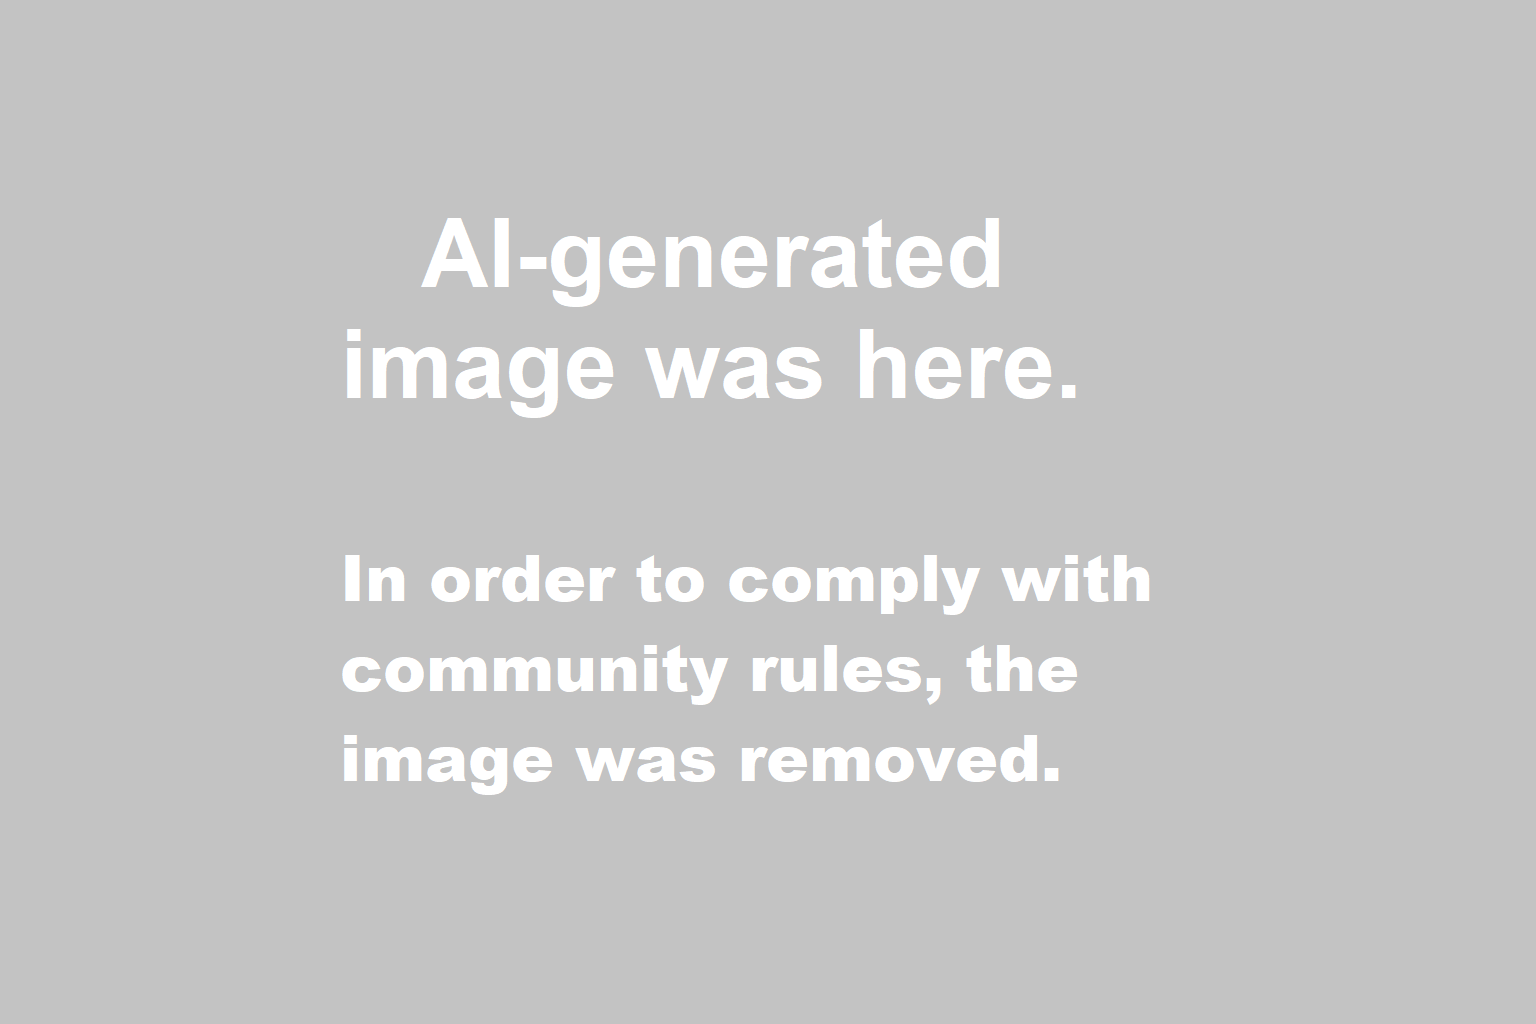
\includegraphics[width=1.4\textwidth]{images/island.png}
		\end{adjustwidth}
		\vspace{1cm}
		{\Large by \@author \par}
		\vspace{0.5cm}
		{\large \today \par}
	\end{titlepage}
}
{
	% no-AI page
	\begin{titlepage}
		\pagecolor{blueRadiance}
		\color{goldStats}
		\centering
		{\Huge \bfseries \sffamily {\MakeUppercase{\@title} \\ \vspace{0.5cm} \Large \subtitle{}} \par}
		\vfill
		\begin{adjustwidth}{2cm}{0cm}
			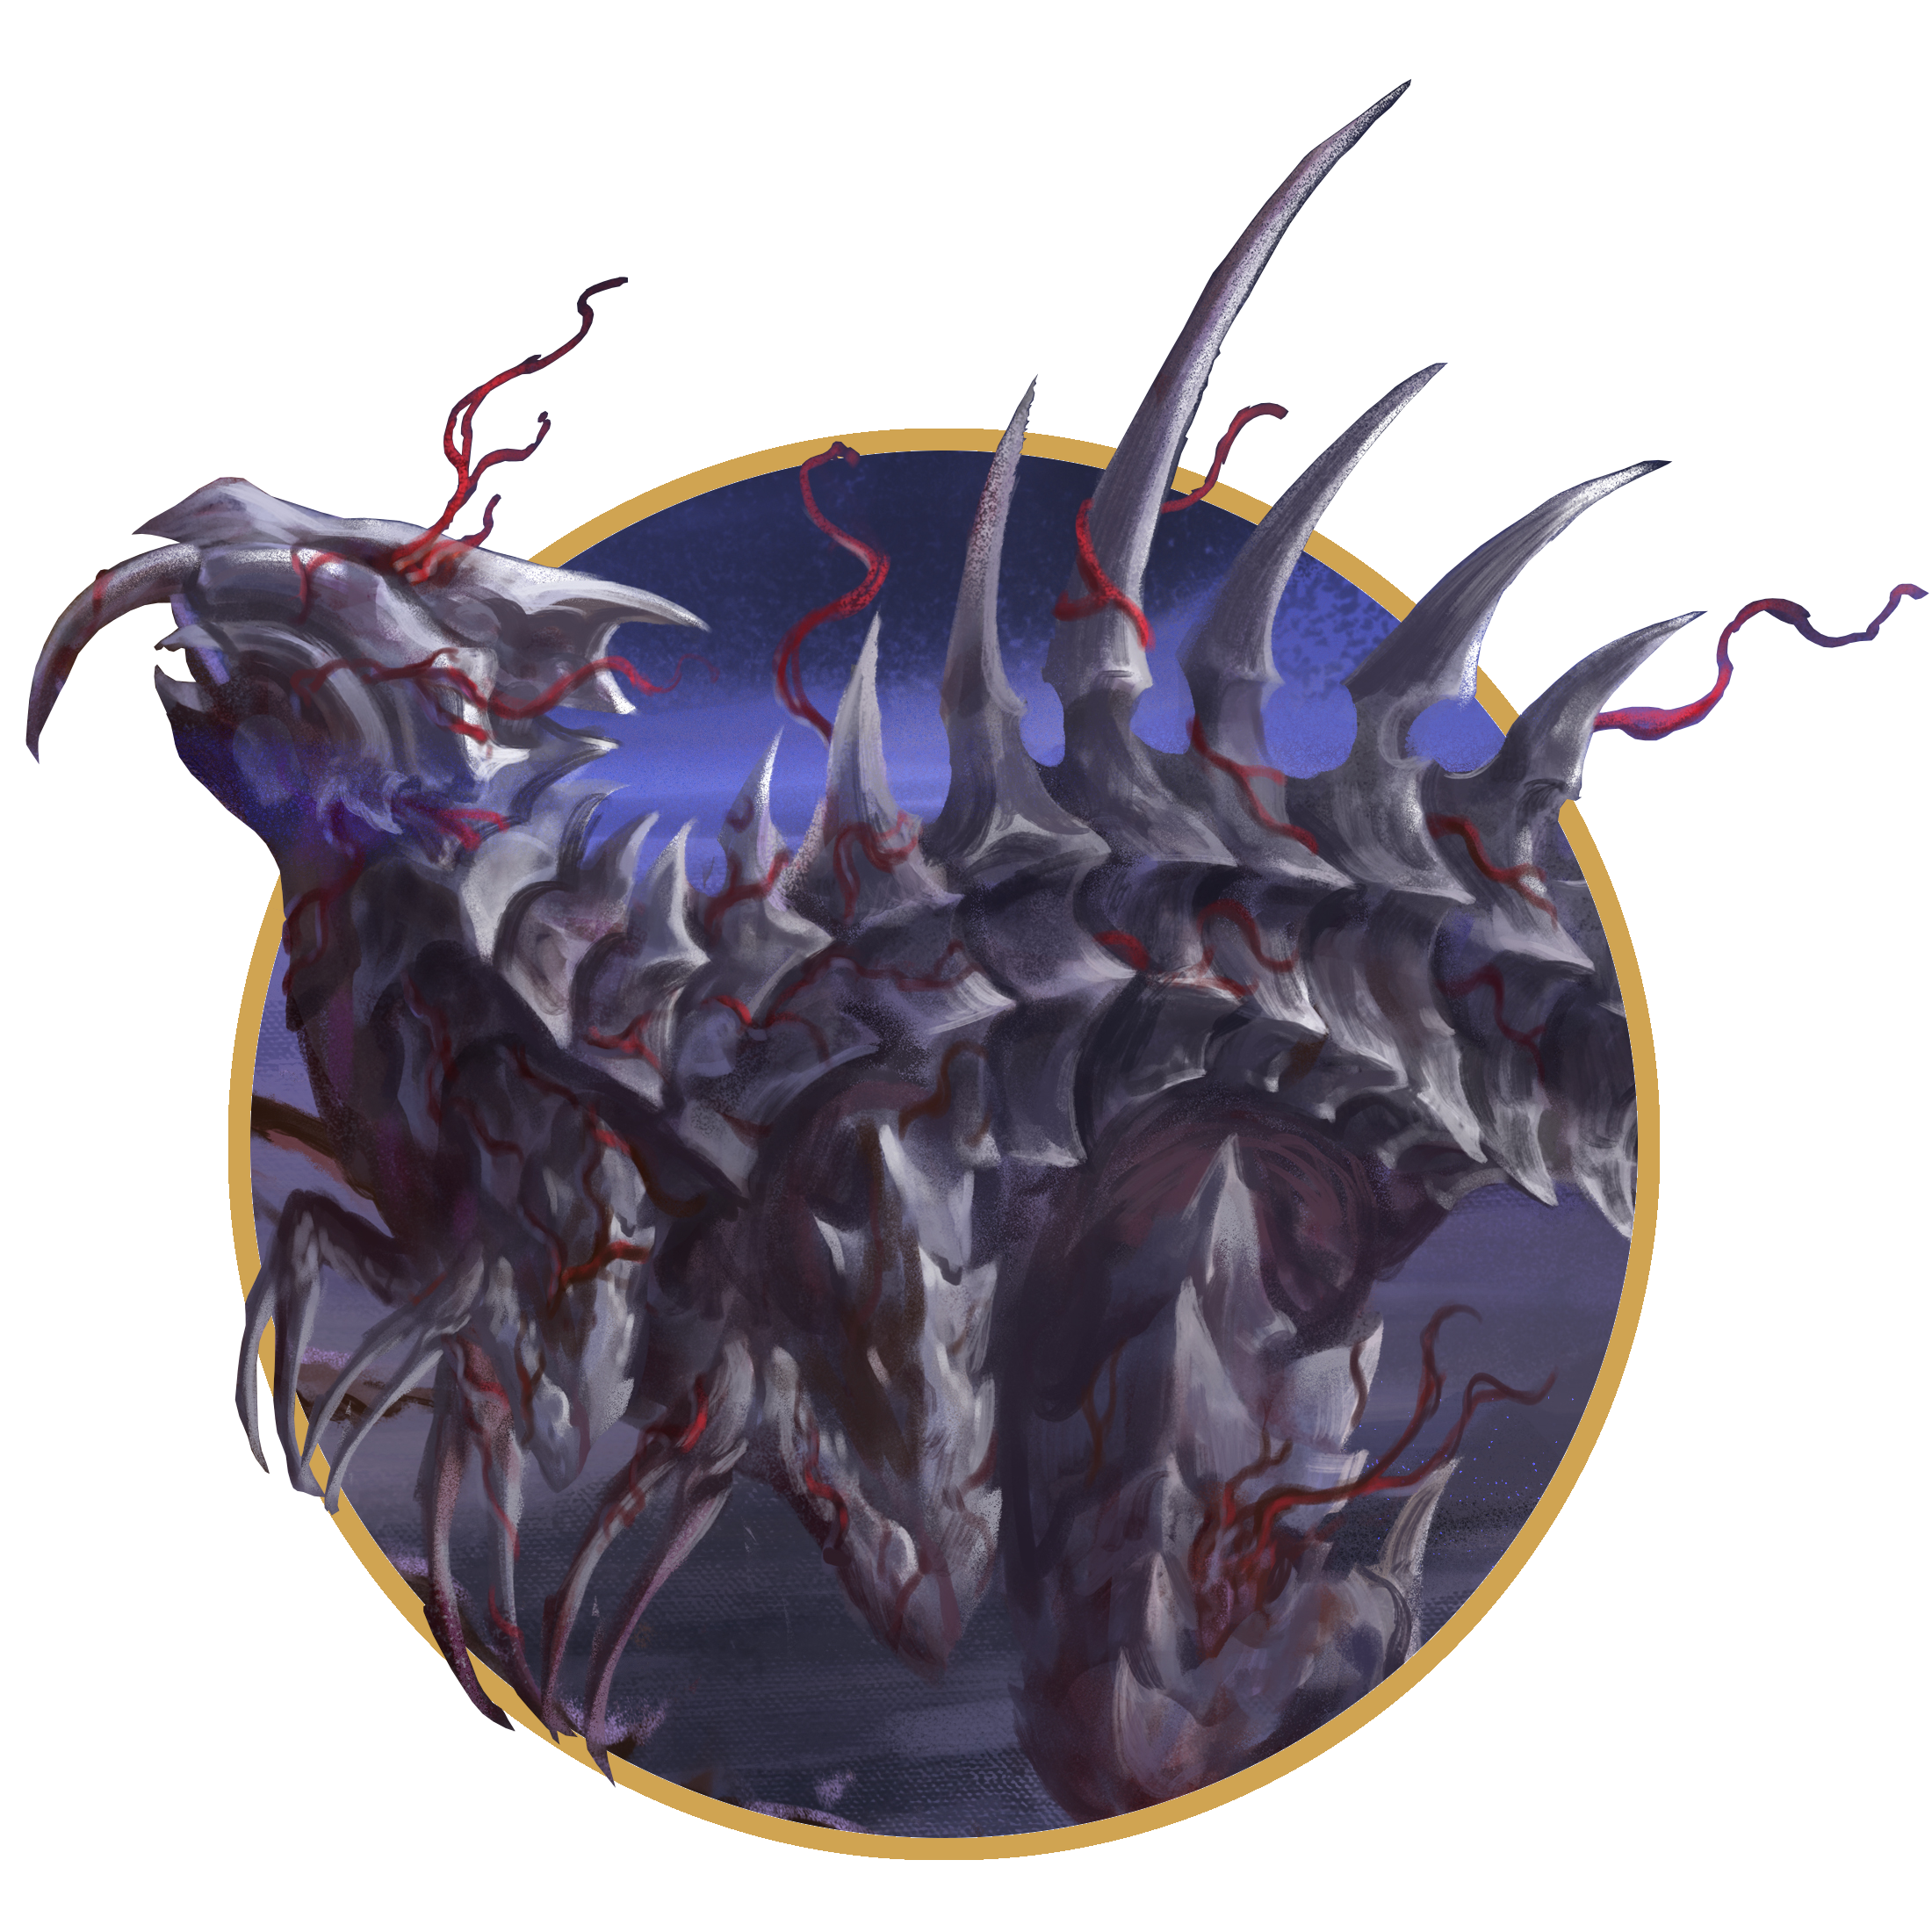
\includegraphics[width=0.8\textwidth]{images/reanimatedWhitespineCover.png}
		\end{adjustwidth}
		\vfill
		{\Large \sffamily by \@author \par}
		\vspace{0.5cm}
		{\large \sffamily \today \par}
	\end{titlepage}
}


\makeatother

\newpage
\pagecolor{white}
	
\begin{center}
	
\includegraphics[width=0.7\textwidth]{images/forUseStormlight.png} \vspace{0.5cm}
	
	
\includegraphics[width=0.7\textwidth]{images/forUseCosmere.png}	
\end{center}

\parbox{9cm}{
	\vspace{1cm}
	\credits
		{Pether.pg} % Designer
		{Pether.pg} % Writer
		{Pether.pg} % Editor
		{Caio Santos} % Artists
}



\vfill

\color{goldStats}\noindent \rule{1.0\textwidth}{2pt}
\begin{center}
	\vspace{0.3cm}
	\color{black} \sffamily 
	This fan content requires the \handbook{} and \bookWorldGuide{} to play.
	\vspace{0.3cm}
\end{center}
\color{goldStats}\noindent \rule{1.0\textwidth}{2pt}

\vspace{0.5cm}
\sffamily \noindent \color{blueRadiance} 
\textbf{\myTitle{}}
\color{black} is unofficial Fan Content permitted under the Fan Content Policy. Not approved/endorsed by Dragonsteel Entertainment or Brotherwise Games. Portions of the materials used are property of Brotherwise Games, LLC~\markC{} 2025 by Brotherwise Games, LLC. Based on The Stormlight Archive\markR{} novels by Brandon Sanderson, copyright~\markC{} 2010, 2014, 2017, 2020, 2024 by Dragonsteel Entertainment, LLC.

\noindent Plotweaver™ Game System \markC{} 2025 Brotherwise Games, LLC.


\begin{center}
	\color{blueRadiance} \textbf{THE COSMERE\markR{} RPG} \color{black} was created by Brotherwise Games and Dragonsteel Entertainment.
\end{center}

% \color{goldStats}\noindent \rule{1.0\textwidth}{2pt}

\newpage
\normalfont
	
	\setcounter{tocdepth}{1}
	\tableofcontents
	
	\renewcommand{\listfigurename}{List of Images}
	\renewcommand{\figurename}{Image}
	\listoffigures

	\twocolumn
	\setcounter{chapter}{-2}
	\chapter{Introduction}


\section{About this book}

\subsection{About me}

Hello! I'm glad to meet you :)

You can call me Pether. I am a fantasy nerd who has played RPGs since childhood. Recently I've dived even deeper into this hobby as I am GMing a campaign for my friends for the past two years. I happily enjoyed various homebrew systems, Dungeons and Dragons, Warhammer RPG, Call of Cthulhu, and now - \cosmereRPG{}.

All my content and RPG resources are free for everybody. I would be happy to play with you, but since I can't, I will gladly share my ideas and notes, perhaps you will find them helpful. You are invited to modify my work to suit your own needs and playstyles. If you share your RPG sessions on youtube please let me know when you play this adventure, I will be excited to see how the story develops for your group!

I hope you will enjoy this adventure. If you would like to virtually hang out or to fuel my various future projects, you can always buy me a coffee using the link below ;)

\url{https://ko-fi.com/pether}


\subsection{Who is it for?}

This campaign is tailored for people who are not familiar with Roshar and Brandon Sanderson’s books. The story starts in Shinovar kingdom, which is the most similar to the classic fantasy setting. Characters originating in there do not require any knowledge about Roshar, storms or spren to start roleplaying.

The story quickly moves from those familiar areas northward, so you can quickly introduce Roshar. Players who know more about the world will be able to shine there.

\subsection{Is it canon?}

No. This is a fan-made campaign and the story presented in here cannot be considered canon. While I did my best to align with official lore of the world, some of the events here might contradict Brandon Sanderson’s vision.

\subsection{How many spoilers?}

The campaign is designed to include as little spoilers as possible. No book character makes an appearance here and the campaign story does not intertwine with the events described in the books.

However, it is impossible to remain fully spoiler-free… The ecosystem of Roshar is quite unique and by playing this campaign players are bound to discover it before reading the books. In particular, the nature of Reshi Islands cannot be avoided here, potentially spoiling one of the chapters in \bookWOR{}.

\subsection{Motivation behind this book}

While browsing official \cosmereRPG{} books I noticed adversaries listed there follow the same pattern - they are either a creatures in carapace, or humans, or nearly-humans in carapace. I wanted to design an adventure with more enemy variety. This book revolves around undead, or at least something similar that could possibly work within Roshar lore.
\section{About This Adventure}
\label{sec:aboutAdventure}

\subsection{Campaign Themes}

This campaign is using themes as listed below. Use this list to determine if you are interested in running this kind of campaign. In the game, you can encounter themes of:
\begin{itemize}
	\item Jungle exploration
	\item Horror
	\item Undead
\end{itemize}

\subsection{Campaign Setting}

Most of the adventure is happening on one of the Reshi Isles. Some of the scenes are taking place in Ksitor (Iri) and players can voyage to Rall Elorim (Iri) and Kurth (Rira). You can start the adventure in Shinovar for an easier Roshar introduction to the people who are not familiar with it.

The story is hardly connected to any events described in the books. This campaign assumes it is taking place alongside the story of “The Words of Radiance”, but GMs can modify a few names of kingdoms and ruling monarchs to set this adventure in any epoch they like, eg. during Silver Kingdoms era, right before the False Desolation.

You can also run this adventure after the events described in official "Stonewalkers" book. You would probably modify a few things (most notably - difficulty level, as the characters would have 7 more levels than initially assumed), but since this adventure starts in Iri (the same kingdom where "Stonewalkers" ends), it should be rather easy to ensure story continuity.

\subsection{Radiant Warning}

Some of the campaign challenges would be trivialized by using Knight Radiant Surges, especially by the healing powers of the Progression Surge. In order to ensure that players won’t skip entire plot lines, to encourage creative problem-solving and to make the tension higher, in many scenes Knights Radiant might attract larkins while using their powers. Those little critters will drain them from the Investiture, interrupting their abilities and preventing their future usage.

Bonding with spren can still occur, but please be aware that this story will focus more on Heroic Path progression - manage players’ expectations accordingly.

The threat of the larkins diminishes after completion of "\nameref{chap:sickGirlDies}". Starting from the next chapter, the characters can freely use full extent of their powers.
\section{Running the Adventure}
\label{sec:runningAdventure}

To run this adventure you will need \handbook{} containing all rules and guidelines on how to run \cosmereRPG{}. This book contains only adventure-specific details and suggestions on how to run it.

\quoteBox{
	You can read (or paraphrase) a text in such a box to your players. Alternatively, you can describe the scene using your own words.
}


Whenever a characters name appears in \enemy{bold}, it means there is corresponding stat block available. You can use it to get more info about the character's attributes and abilities.

Items appearing in \loot{bold italic} have special rules you can find at the end of this book.

\reasonBox{
	Boxes like this will help you understand the reason behind some of the design choices. Those have no impact on the game, but they may help you modify some elements of the adventure if you so choose.
}

\ptrBox{
	When a plot might allow for certain Radiant Spren to be attracted by player's actions, that will be indicated by such a box. However, use your own judgment whenever a players does something not accounted by this book.
}

If you are using this book in electronic version, it has also several quality-of-life improvements to make your life easier when you navigate this book:

Whenever a name of a chapter or section appears (eg. "\nameref{sec:aboutAdventure}"), you can click on it to quickly go to the chapter in question.

All characters' names (eg. \npcMedic{}) are links that lead to \hyperref[personae]{Dramatis Person\ae} chapter, where all the NPCs are listed.

Items (eg. \lootRogueShardblade{}) and adversaries (eg. \enemyDrunkenSailor{}) are also links that will lead you to the page with their unique rules. 


\subsection{Adjusting Difficulty}

This book assumes your players will form a party of 4 characters starting at 1st level. However, it is perfectly fine to have a different size of your group and/or to start playing at a different level (eg. because the characters already shared a different adventure together). Also, it is possible that challenges presented in this book are not aligning with strong suits of the party.

If you see that the balance is a bit off, feel free to adjust the difficulty. You can change a number or tier of the enemies, modify endeavors' requirements or weave some other changes into the story.

\subsection{Handling Canon}

Despite treating original source with respect, this adventure is not canon. While playing the game your primary focus should be fun. For everyone, "fun" means something different - either following official lore to the letter, creating your own touching story, or just hitting bad guys with your sword. Make sure you know what is fun for you and your group and make it your primary objective. If that means modifying this adventure or straying away from the canon - go for it!

You can find more information on that topic in “Canon and Continuity” section of \handbook{}.

\subsection{Playing with Radiants}

Please keep in mind, that this adventure greatly limits Radiants' abilities with larkins swarming the area. However, if a player wants to play as Knight Radiant despite it (for example - to tell a story about their relationship with the spren) this book will provide some opportunities to enable this kind of story. Just make sure your players are aware of the limitations that might hinder some of their abilities.

\subsection{Playing with Singers}

This story does not focus on conflict with Singers. If a player wants to play with a Singer heritage, it is perfectly acceptable. This book assumes the story is happening sometime along \bookWOR{}, but it provides little details related to Singer mechanics and it leaves it up to you to fill those gaps if required.

If one of your players wants to play as a Singer, please discuss with them what kind of story do they want to tell and adjust this adventure accordingly. You can run it before, after, or just at the moment of the Everstorm reawakening, or in another era entirely - the core of this story will remain unchanged, but various NPCs may react to the singer differently depending on the date you choose.




\section{Adventure Summary}

\subsection{Chapter 0 Summary}

Characters start their adventure on the ship from Shinovar, sailing towards Kasitor. Consider this a tutorial chapter to introduce players to the world of Roshar, mechanics of the game and roleplay in general. You can skip it if you are playing with a more experienced group.

\subsection{Chapter 1 Summary}

While in Kasitor, characters learn about a lost Reshi Isles expedition. They board a ship and sail north, to learn about the expedition's fate and search for survivors. When they reach the shore of \theIsland{} island, they notice strange red vines, unique for it. While searching the island, they meet \npcMedic{}, herdazian man leading a pack of Axehounds fighting with a Whitespine.

\subsection{Chapter 2 Summary}

\npcMedic{} leads the party to his camp. Here characters meet a sick Thaylen girl that \npcMedic{} is attending with his medical knowledge. He asks the party to find some herbs he needs to help the sick girl and perhaps find some information about the rest of the expedition he left behind. When characters return to the camp, they are attacked by a few Axehounds. They recognize the beasts that fell earlier, now returned back to life and overgrown with scarlet vines.

\subsection{Chapter 3 Summary}

After learning about the strange vines growing over slain beasts, \npcMedic{} asks characters to gather more information about them. He asks for some samples and suggests learning from the local Reshi village. Once it is discovered that the vines are revered by locals as a holy plant that can empower people and reanimate dead, \npcMedic{} suggests using them for treatment of sick Thaylen girl, without which she is doomed to die.

\subsection{Chapter 4 Summary}

Identifying red vines as a threat for nearby islands, characters may travel to gather some support to deal with the situation. Upon their return, they witness the danger growing out of hand. They must hurry to resolve the threat before it is too late…

\subsection{Chapter 5 Summary}

The party ventures deep into the ancient Reshi shrine to face the spren responsible for the plague of spreading vines, \npcSprenVines{}. Regardless of characters’ approach to the threat, the Reshi Isle will be changed forever.

\section{Dramatis Person\ae}
\label{personae}

Following NPCs appear in the adventure:

\begin{itemize}
	\item \npcShinCaptain[s] - Shin ship captain that sails to Kasitor.
	\item \npcShellSeller[s] - young girl selling shells in Kasitor.
	\item \npcDrunkenSailor[s] - a \enemyDrunkenSailor{} in Kasitor.
	\item  \npcWorriedWife[s] - wife of \npcCapturedExplorer{}, met in Kasitor.
	\item \npcMedic[s]{} - Herdazian medic treating \npcSickGirl{}.
	\item \npcBabsk[s]{} - Thaylen explorer, babsk of \npcSickGirl{}.
	\item \npcSickGirl[s]{} - young Thaylen explorer, affected by sickness.
	\item \npcCapturedExplorer[s]{} - expedition member, Iriali, captured by Reshi.
	\item \npcDeadExplorer[s]{} - expedition member, Natan, died at the entrance to the temple.
	\item \npcReshiPriest[s]{} - Reshi priest devoted to the island of \npcSprenVines{}.
	\item \npcReshiKing[s] - Reshi king on Kadrix.
	\item \npcReshiInterpreter[s] - interpreter of \npcReshiKing{}, speaking on his behalf.
	\item \npcArtifabrian[s] - Veden artifabrian working in Kurth.
	\item \npcRogueShardbearer[s] - a \enemyRogueShardbearer{} operating in Rall Elorim.
	\item \npcSprenVines{} - ancient spren controlling the Red Vines on the island.
	\item \npcHoundLady{} - pretty axehound with red ribbon, guards \npcSickGirl{}.
	\item \npcHoundScratch{} - axehound with green collar, very friendly, loves pets and scratches.
	\item \npcHoundFetch{} - young axehound, loves playing with his toy skyeel, often attracts joyspren.
	\item \theIsland{} - Reshi Tai-Na greatshell, the island where the story takes place.
\end{itemize}
\section{Before Starting the Campaign}

Here are some tips and suggestions intended for the GM. Following them is not mandatory, but it might help you run the game.

\subsection{Required Knowledge}

Since the story does not touch on any events from \bookSA{} and the characters start from Shinovar, they are not required to know much about Roshar world or story presented in the books.

Of course, you as a Game Master will need to know rules of \cosmereRPG{} and enough about Roshar world to paint the picture for your players.

\subsection{Read the Adventure}

Unless you mastered improvisation, spend some time to familiarize yourself with the adventure. It will help you adjust the story to players' characters and their personal stories, as well as it will allow you to quietly foreshadow key elements of the plot.

\subsection{Players’ Expectations}

Inform players that the adventure will revolve around Reshi Isles and that Radiant powers will be limited. Discuss with players what are their expectations for the game. Consider following questions:
\begin{itemize}
	\item How serious should the adventure be?
	\item What topics players would prefer to avoid during the game?
	\item Is there anything the players would like to see in the game?
	\item Are the players comfortable with their characters dying?
	\item Are the players comfortable with characters' romance, nudity or other sexual content?
	\item If you are of age - should your group allow alcoholic drinks?
	\item What rule variants should be in effect?
	\item How often should your group meet and how long should a single game session take?
	\item How should you handle situations when one player cannot attend a game session?
\end{itemize}

Gathering answers to those (and similar) questions is not a requirement, but it will tell you about players’ hopes for the game and it will help you create a better experience for the whole group.

\subsection{Create Player Characters}

Unless your players have their characters ready after previous adventures, they must create a new party. This book contains several pre-made character sheets you can use in your game (see \hyperref[chap:exampleSheets]{Appendix \ref{chap:exampleSheets}}.), but you should encourage players to create more personalized heroes for the story.

While creating new characters, you might want to follow those guidelines:
\begin{itemize}
	\item encourage Human Ancestry, unless the player is familiar more complex Singer rules and culture.
	\item encourage Shin culture, unless the player is already familiar with the world of Roshar.
	\item another cultures relevant for the story include: Iriali, Riran, Reshi, Herdazian and Thaylean.
	\item share \hyperref[backstoryIdeas]{\textbf{Character Backstory Ideas table}} with your players for possible inspirations for characters, their motivations and goals for the story.
	\item warn players that Radiant Paths might be more challenging to play this adventure. While the story does not prevent playing with those, some of their powers are limited and players should be aware of that before choosing those paths.
	\item if a player plans playing as Knight Radiant, make sure you know what spren to introduce in the story.
\end{itemize}

\subsection{Character Relationships}

Allow players do determine how their characters know each other and what is the reason they are traveling together. Establishing characters' relations before the adventure start will make it less likely the heroes will be motivated to split the party and follow their own goals.

You can add more details to character's relationship by requesting each player to ask about some specific details two other characters. Players can think of their own questions they want to ask each other or they can choose something from the list of below:

\begin{itemize}
	\item "Once you shared with me your strange, irrational fear you never told anyone else. What was it?"
	\item "We have one thing in common what we would never guess we could share. What is it?"
	\item "Once you told me you wanted to travel with me to some remote location. Where would that be?"
	\item "You often call me a silly name. What's the name and why did you start using it?"
	\item "Your religious practices differ from those commonly observed in your lands. Why?"
	\item "I noticed you play with some small item. What is it and why do you carry it?"
	\item "You told me once that you lost someone close to you. Who was it and what would you give to get them back?"
	\item "You once told me there are worse fates than death. What did you have in mind?"
	\item "What is the case that you are willing to die for?"
\end{itemize}

\subsection{Character Backstory}

Encourage players to write a short character backstory to better root them in the world and the story. Consider if any NPCs from those backstories could make an appearance in this adventure and how they can enrich the story. You can modify scenes described in this book to include those NPCs, for example:
\begin{itemize}
	\item additional NPC can join the expedition and be lost on the island
	\item an NPC known to players’ characters might be sick and tended by Melio
	\item Reshi village might be joined by someone from the player’s backstory
	\item an old friend might be met while searching for aid
\end{itemize}



\section{Unique Rules and Events}

The game follows original \cosmereRPG{} rules with a few unique additions, specific for this campaign:


\subsection{Ravenous Larkins}

The Reshi Island, where most of the adventure is taking place, is swarming with larkins. Each time a character uses Investiture, spawn \enemyLarkin{} into the scene. The larkin attacks the character, feasting on their Investiture, until there is nothing left. When no player can be targeted with larkin's Drain Light ability, the creature flee.

If a player repeats Investiture usage later, spawn more larkins and/or make them more aggresive each time.

If a larkin appears outside of combat, there is no need to start the fight - allow it to Drain Light and fly away. If spawned during combat, however, those creatures are more aggressive: while their focus is on using Drain Light and staying alive, they can also attack player characters with their Bite action.

All larkins are immune to Red Vines influence (see below).

\reasonBox{
	Limiting Investiture abilities can create unique challenges for the players and make the game more interesting. However, the main reason for this feature is to prevent healing NPCs using Progression Surge in later chapters - Radiant abilities would make that part of the plot boring and trivial. 
	\newline
	Despite real significance in the future parts of the story, introduce Larkins earlier to properly warn the players about that threat to Radiant abilities.
}


\newpage % manual newpage to micromanage page layout

\subsection{\abilityVinesName}
\label{ssec:ruleVines}

During the adventure, the PCs can encounter strange, red vines growing on the island. If they are allowed to overgrow a living creature, that creature gains the following ability:

\abilityVines{}

If you add this feature to an existing stat block, remember that Strength affects Physical Defense, Health and some of the skills - those in turn can affect attack and damage bonuses. Pay attention, that Strength affects total Health once every tier - enemies on higher tiers will receive Health bonus several times.

Unknown to everyone, the Vines are a variety of rockbuds without their own shells - instead they inhabit carapaces of slain creatures. They are controlled by a spren from the ancient temple, \npcSprenVines{}. Creatures affected by this ability are influenced by the spren and want to follow its will. Given time, the Vines will creep inside host's body, causing more and more pain, and, in the end - gruesome death, giving birth to a new Husk.

\reasonBox{
	Red Vines are an alluring promise of strength, power and immortality that leads the desperate to their doom. They are the magic that goes horribly wrong because the caster did not fully understand it. Reveal any information relating to it slowly, in the pace of whole story.
	\newline
	If players are desperate to use the scraps of knowledge they have, they can invite the Red Vines enhancement. However, be prepared to introduce negative consequences slowly creeping in as the Vines themselves.
}


\subsection{\abilityHuskName}
\label{ssec:ruleHusk}

Red Vines are a rockbud variant that lacks it's own protection. Instead, the plant uses carapace of dead animals as a shell. While overgrowing the corpse, the Vines can animate it like a puppet, allowing for locomotion and self-defence. Creatures under this effect gain following ability:

\abilityHusk{}
\newpage % manual newpage to micromanage page layout

Such husks loose all their previous identity and cognitive abilities. They cannot communicate nor understand any communication attempts. They are driven by anger and desire to create more corpses for the Vines to grow into. They fight mercilessly without any will to preserve own existence. While not fully alive, it is difficult to kill them, and any attempts may just cause their body to split into smaller parts. 

\reasonBox{
	Reanimated Husks are my attempt to bring undead into the world of Roshar. They are mindless and deadly. Their existence is a huge threat to the Island and eliminating it will eventually be players' main goal. Try to make them as gruesome, hideous, grotesque and dangerous as possible.
}
\section{Handling Death}

It is possible a character will meet their demise during this adventure. Here you can find some suggestions on how to handle those situations.

\scriptedOption{Introduce a new character.}{
	There are several opportunities in the story to introduce another character and allow them join the party to fill the void remaining after recently slain companion.
}

\scriptedOption{Encounter with \enemyReanimatedPerson{}.}{
	If the PC died on the island, it is quite possible that \npcSprenVines{} will use the Red Vines to reanimate their body as \enemyReanimatedPerson{}. The party can encounter their companion in the later parts of the story, this time, however, as a reanimated corpse.
}

\scriptedOption{Another chance.}{
	If a PC would be slain by an enemy with \abilityVinesName{} ability, instead you can show the Vines infestation spreading to the flesh of the PC - thin Red Vines sprouting from character's body. Such character would get \abilityVinesName[2]{}, receiving some attribute boosts, but treating other infected creatures as allies and raising as \enemyReanimatedPerson{} the next time they would die again, spawning another enemy for the rest of the party during combat.
}

\scriptedOption{Part of the journey.}{
	In the final part of the story it is expected some of the characters may die. Don't run from it, don't sugarcoat it, don't avoid it. Allow the PC to sacrifice themselves for a bigger cause and weave that death into the story. 
}



\onecolumn

\begin{table}
\centering
\label{backstoryIdeas}

\begin{tabular}{p{2.8cm} p{6cm} p{3cm} p{3cm}}
	\hline
	\color{black} Starting Path & \color{black} Reason & \color{black} Questions & \color{black} Goals \newline \\ \hline
	
	\color{black} Envoy or Hunter
	&
	\color{black} You enjoy the alluring call of freedom - wind in your hair, the song of the waves in your ears and the sight of the endless horizon... And the call of Reshi Islands is the most tempting one. \newline
	&
	\color{black} Is there any reason you yearn for freedom? What are you leaving behind?
	&
	\color{black} Impress the Reshi people and become one of them.
	\\ \hline
	
	\color{black} Scholar or Envoy
	&
	\color{black} Unexplored wilds of the Reshi Islands hide many mysteries waiting to be uncovered. Fauna, flora and folklore of those areas are barely researched and you are eager to learn more about them! \newline
	&
	\color{black} Is there anything specific you would like to research? Why?
	&
	\color{black} Write a paper with your findings.
	\\ \hline
	
	\color{black} Leader or Warrior
	&
	\color{black} Some people prepare for a voyage to the Reshi Islands. You don't really care about the Islands themselves, but those travelers need your help! \newline
	&
	\color{black} Why do you want to help those people in particular?
	&
	\color{black} Ensure the safety of the voyage.
	\\ \hline
	
	\color{black} Agent or Warrior
	&
	\color{black} You received information about an expedition ship being lost in the area of nearby Reshi Isles. You are ready to sell your services to them. Or, if it is too late for them, perhaps something valuable can be found in the remains? \newline
	&
	\color{black} Why do you are desperate to get money?
	&
	\color{black} Ensure profitability of this mission.
	\\ \hline
	
	\color{black} Leader or Scholar
	&
	\color{black} Reshi people are known for their lack of proper education. You are sure you can make their lives and futures better with your knowledge and you are eager to share it with them. \newline
	&
	\color{black} What drives you to educate Reshi people?
	&
	\color{black} Start school on a Reshi Isle.
	\\ \hline
	
	\color{black} Agent or Hunter
	&
	\color{black} Legends say about an ancient temple lost in the jungles of the nearby Reshi Island. Whatever is lost within it, must be waiting to be discovered and reclaimed! \newline
	&
	\color{black} What do you hope to find in the temple?
	&
	\color{black} Find the temple and the riches it contains.
	\\ \hline
	
\end{tabular}
\end{table}
\twocolumn

	\renewcommand{\thefigure}{0.\arabic{figure}} 
	\chapter{Chapter 0 - Welcome to Kasitor}
\label{chap:tutorial}

\setcounter{section}{-1}
\section{Running This Chapter}

Consider this chapter a tutorial and introduction to Roshar, \cosmereRPG{}, basic game mechanics and RPG in general. If you are playing with more advanced players, you can easily skip this chapter and start with "\nameref{chap:chapter1}".

\subsection{Character Advancement}

It is assumed the characters start this adventure at level~1. Do not advance characters at the end of this chapter.

\section{Roshar, the World of Stone and Spren}

This might the the first time the characters (or even players) step into the grand Roshar. Here, they can be introduced to spren, parshmen, and other unique aspects of the world. 

\reasonBox{
	If your plying group enjoys more roleplay aspects of the game, don't rush through those scenes. Instead, allow players to react to and interact with the world and NPCs.
}

\subsection{Adventure Starts}

You can start the adventure by reading the following:

\quoteBox{
	Foam-Daughter-Waves sails peacefully through shining surface of the sea. Captain \npcShinCaptain{} agreed to take you on his ship and now you are farther from home than ever before. 
	\\ \\
	Your journey started in Ayabiza on the north shores of Shinovar and if spren allow it, soon you will reach Kasitor, where Lorseth hopes to find some profitable trade.
}

\roleplayBox{\npcShinCaptain{}}{
	\roleplayTips
	{Curious, supporting.}
	{Make a good trade, help his friends.}
	{\npcShinCaptain[s] has a light skin and brown hair.}
	{\npcShinCaptain{} is a trader from Shinovar. He loves traveling across the Roshar and meeting new people in all those places he visits. Very loyal to his friends and fellow Shin folks, he is eager to show them the wonders of the world.}
}

\subsection{Windspren Chase}

Once the ship sails far away from the shores of Shinovar, read the following:

\quoteBox{
	Suddenly, you feel a gust of wind and several light-blue ribbons of light appear in the air. They scatter around the ship's sail and fade as quickly as they appeared. With following gust, new group of lights appear.
	\\ \\
	"Beautiful, aren't they?", asks \npcShinCaptain{}. "Is it the first time you see a windspren?"
}

A character may wish to interact with windspren - worship them or start chasing the wind alongside them. If they do, read the following:

\quoteBox{
	One of the spren separates from the group and flies towards you. The ribbon of light floats in front of your face and you get a feeling it regards you with child-like curiosity. 
	\\ \\
	A moment later it whirls a few times around your head and flies away as a blow of wind ruffled your hair. You could swear the spren was giggling."
}

\reasonBox{
	You can introduce more nature or emotion spren for your players. Show some luckspren flying alongside the ship, flamespren near the candles, anticipationspren showing when players are looking at the horizon, etc.
}

\creditedArtFigure{width=0.45\textwidth}
					{images/firstTimeSailing.png}
					{AI}
					{Shin girl seeing spren for the first time.}
					{fig:firstTimeSailing}


\subsection{City of Stone}

When the ship reaches Kasitor, read the following:

\quoteBox{
	You approach the great city of Kasitor, the greatest city you've seen in your life. Also, a city built entirely on stone. Blasphemy!
	\\ \\
	From the deck of the ship, you see people walking, strolling, rushing, trading on the stone ground. On the sacred, stone ground!
}

Allow players to react to the people walking on the stone, something unbelievable for a Shin. Based on their reaction, you can show shockspren, angerspren, or other spren appearing near them.

After that, read the following:

\quoteBox{
	Suddenly, a whirl of water rises from the surface of the water. An enormous being made of water raises its hands of waterfalls and reaches towards the city. 
	\\ \\
	Is it a spren, offended by the stonewalkers? Will blasphemy meet its demise?
	\\ \\
	"Don't worry", \npcShinCaptain{} says. "The people are safe. It is Cusicesh, the Protector of the city. His appearance means we made it in a good time!"
}





\section{Swordfight Training}

When the ship docks, read the following:

\quoteBox{
	"Wait a second!", \npcShinCaptain{} stops you. "Those lands are less safe than Shinovar. Even those who add must know how to defend themselves. Here, catch this!" He adds as he throws a wooden training sword in your direction.
}

This is an opportunity to learn basics of combat in \cosmereRPG{}. The fight is perfectly safe. Assume the training swords do 1 damage on hit, 0 on graze, and the damage heal quickly as they are just a few bruises.

\npcShinCaptain{} is \enemyExpert{} - has Physical defense of 12. His attacks receive +2 bonus to hit. A single sparring fight is made until one person was hit 3 times. Encourage creative application for surroundings and various combat actions.

\section{Shell Seller}

If a character decides to disembark and see the city, read the following:

\quoteBox{
	When you step on the stone ground of the port, a little girl approaches you. Her hair looks as if made of gold, and she has gold tattoos on her skin.
	\\ \\
	"Would you like to buy a shell?", she asks with a cute voice.
}

\npcShellSeller[s] is a young Irali girl. She sells sea shells on the sea shore. If a player inspects her collection, they can find shells of various shapes, sizes and colors, as well as various hand-made jewelry. The girl tells about amazing properties each of them has.

If a character is interested in something in particular, \npcShellSeller{} tells them a price of the item. It is much too high for a character at this level (25 marks should be high enough for 1st level characters, but she is a skilled trader and can adjust the price if she can see the buyer is richer than that).

Characters can start a conversation with \npcShellSeller{} to haggle the price down.
\conversationDefence{\npcShellSeller{}}{12}{14}{4}
She can be easily interested with some curiosities from Shinovar, but she will spend 1 focus to resist PC's counter-offers.
\conversationEnd{\npcShellSeller{}}{1}

Once the conversation is over, she presents her final offer. For each focus \npcShellSeller{} spent during the conversation, lower the price by 25\%.

\roleplayBox{\npcShellSeller{}}{
	\roleplayTips
	{Cute, enterprising.}
	{Sell shells at the best price.}
	{\npcShellSeller[s] is a young Iriali girl with golden skin, eyes and hair. Her arms are decorated with golden floral patterns.}
	{\npcShellSeller{} is starting her trade from the earliest years. She is a proud owner of jewelry selling stand, mostly focusing on pretty shells. She is curious of the world and loves hearing stories about the places far away. Each customer is a new hope for something interesting happening. }
}

\creditedArtFigure{width=0.5\textwidth}
					{images/shellSeller.png}
					{AI}
					{\npcShellSeller{} selling shells.}
					{fig:shellSeller}

\section{The Drunken Skyeel}

A character may wish to visit port tavern, The Drunken Skyeel. When they enter, read the following:

\quoteBox{
	The tavern hosts few patrons at this hour. The owner cleans some glasses with lazy movements, and the tavern's pet, an old skyeel, currently sleeps in his nest under the ceiling.
	\\ \\
	One of the guests, a Thaylen sailor with long, white and ruffled eyebrows, approaches you. "Do you play?", he asks, shuffling a card deck.
}

\npcDrunkenSailor[s] is a \enemyDrunkenSailor from Thaylenah. Characters can enter a gambling endeavor with him. To start the game, a character must pay 10 marks. Possible approaches to this endeavor may include:

\scriptedOption{Bluffing}{
	A character may bluff about their hand with \skillCheck{13}{Deception}.
}

\scriptedOption{Guessing opponent's hand}{
	The deck is not shuffled between rounds. A character may attempt \skillCheck{12}{Deduction} to determine what cards their opponent may have.
}

\scriptedOption{Watching for cheating}{
	A character may attempt \skillCheck{10}{Perception} to make sure the other player does not cheat.
}

\scriptedOption{Cheating}{
	A character may also cheat with \skillCheck{15}{Thievery}. If the check is failed, proceed to \fullref{sec:tutorialFightNormal}.
}

\subsection{\pursuitResolveHeader}

\pursuitReq{5}{3}

\textbf{Success.} A character won 20 marks. Proceed to \fullref{sec:tutorialFightNormal}.

\textbf{Failure.} Their money was lost. The sailor smiles and invites them to another game.

\roleplayBox{\npcDrunkenSailor{}}{
	\roleplayTips
	{Drunk, aggressive.}
	{Drink more and start some fights.}
	{\npcDrunkenSailor[s] is a sailor from Thaylenah. He is a mess - his clothes are dirty and wet, his eyebrows are all over the place}
	{\npcDrunkenSailor{} is having too much money for his own good. Currently in between the jobs, he has nothing better to do than drink away all his money and pick up some fights along the way. He is too drunk to know any better.}
}


\section{Bar Fight}
\label{sec:tutorialFightNormal}

When \npcDrunkenSailor{} lost a game or spotted a cheater, read the following:

\quoteBox{
	"You cheated!", the sailor shouts, flipping the table. "I will teach you never to cheat again!"
}

\enemyDrunkenSailor{} attacks the characters. He is too drunk to realize his odds and he will fight to the end. If the party has too much trouble in the fight, the barman may join and end it by knocking down the aggressor.

This is the opportunity for the party to experience a real fight. Remind the players about graze mechanics and allow the aggressor to deal some damage to better explain healing in the game.

\section{Worried Woman}

If you need a plot hook for the characters to proceed to the main part of the adventure, you can read the following:

\quoteBox{
	A young Irali woman approaches you. Her eyes are dark and tired.
	\\ \\
	"Excuse me, are you a sailor?", she asks. "Have you seen my husband? He sailed with Thaylen expedition and should be back by now, but all contact with his ship was lost..."
}

\npcWorriedWife[s] is worried about her husband, \npcCapturedExplorer{}. She offers 50 marks for each character if they can find him and bring to safety. This should give the party a nudge they need to board the ship and start the main part of the adventure. 

\npcCapturedExplorer{} is currently captured by Reshi people and can be found in their village (see \fullref{ssec:imprisonedSailor}).

Players can persuade \npcShinCaptain{} to take them north for expedition search, or they can find another ship sailing in that direction. It is up to you (and players) what solution will be applied to continue the adventure.

Whatever means of travel are secured, this book does not use any NPCs from Kasitor in later chapters. Remember to include them and secure story continuity if there are strong reasons to believe they should appear (eg. ship captain and the crew).


\roleplayBox{\npcWorriedWife{}}{
	\roleplayTips
	{Worried, fearful.}
	{Find her husband.}
	{\npcWorriedWife[s] is an Iriali woman with golden skin and eyes and tattoos. Her golden hair are in messy state, so is her dress.}
	{\npcWorriedWife{} lives in Kasitor. Her husband, \npcCapturedExplorer{} works as a sailor for a Thaylen expedition, but contact with them was lost some time ago. She is terrified about the fate, that could meet the expedition.}
}

\reasonBox{
	You can use another plot hook that would fit better the story of your characters.
	\\ \\
	You can also scatter more information about the lost expedition in this chapter - some gossip in the tavern, or inpatient NPCs in the port.
}


\section{Journeying Onward}

Once your players feel more comfortable with the rules and the world, proceed to the next chapter.
	\renewcommand{\thefigure}{\thechapter.\arabic{figure}} 
	\chapter{Chapter 1 - Life Before Death}
\label{chap:chapter1}

\setcounter{section}{-1}
\section{Running This Chapter}

This chapter is a classic travel adventure. Characters face some perils during their voyage and for the first time they see Reshi Islands, where they'll face some enemies in combat, but nothing too dangerous.

While running this part, start foreshadowing the Red Vines, but don't provide too much information about them yet.

In the final fight of the chapter, make sure \npcMedic{} gets hurt and some of his Axehounds get slain, but don't pose lethal danger to the players.

\subsection{Character Advancement}

Characters start this chapter at 1st level and advance to 2nd level after saving \npcMedic{}.

The following decisions offer opportunities to introduce spren, strengthen spren bonds, or swear Ideals:
\begin{itemize}
	\item How the PCs act during the travel.
	\item How the PCs react to the exotic flora of Reshi Island.
	\item How the PCs help \npcMedic{} in the face of danger.
\end{itemize}

\section{Sailing North}

Start the adventure with the following:

\quoteBox{
	Your ship dashes through the waves as you are sailing north. The windspren are chasing your vessel and the anticipationspren are streaming around you - what awaits you behind the horizon?
}

\subsection{Plot Hook}

Unless you started the adventure with "\nameref{chap:tutorial}", add the following to the introduction:

\quoteBox{
	You embarked on this ship with a goal to find a lost Thaylen Expedition. All contact with them was lost several days ago and you are now racing time to save those poor souls from any dangers that may lurk on the islands of the Reshi Sea. And perhaps - to earn some spheres in the process.
}

\reasonBox{
	If you are running this adventure alongside some bigger campaign, you can introduce your own plot hooks instead. Perhaps the characters are already sailing on the Reshi Sea for some other reason and they will encounter the lost expedition by accident, starting a side quest spanning for 5 character levels? You can adjust the reasons for the party to travel to your taste and the backstory of the party.
}

\subsection{Search for the Island}

The characters must find tracks of the lost expedition. You can run this as an endeavor. The search may take several days - consider presenting this endeavor as a montage of small scenes happening during the travel. Possible approaches to the endeavor may include:

\scriptedOption{Reading the map.}{
	One of the characters may have a map with marked expedition's path. Using it requires \skillCheck{10}{Deduction} to properly determine where the expedition might have been lost.
}

\scriptedOption{Ship navigation.}{
	One must know their way with the ship to properly sail on the seas. \skillCheck{15}{Lore} can be used to determine if a character knows how to work with the ship.
}

\scriptedOption{Reading the wind and waves.}{
	The sea can be unpredictable. If a character knows how to read its mood, they can attempt \skillCheck{12}{Survival} to help navigate to safety.
}

\scriptedOption{Hiding from the highstorm.}{
	Though this far west the storms are not as devastating, it is still good idea to avoid them. Use \skillCheck{10}{Survival} to check if a character successfully avoided the highstorm.
}

\scriptedOption{Asking local people.}{
	Perhaps someone saw the expedition ship? Use \skillCheck{7}{Persuasion} to verify if you can get some information from the nearby Reshi Islands
}

\scriptedOption{Spotting the ship.}{
	A character can attempt \skillCheck{12}{Perception} to see if they can spot the expedition ship.
}

\scriptedOption{Pure luck.}{
	Sometimes all you can count on is your luck. A character may roll d20, a result 10 or higher means they were lucky enough with their search.
}

\subsection{Opportunities And Complications}

\oppCompTable{
	\oppCompRow{\iconOpp[15pt]}{You managed to catch some delicious fish for dinner.}
	\oppCompRow{\iconComp[15pt]}{The sea is not for you. You got sea sick.}
}

\creditedArtFigure{width=0.45\textwidth}
					{images/island.png}
					{AI}
					{Approaching \theIsland{} Reshi Isle.}
					{fig:island}


\subsection{\pursuitResolveHeader}

\pursuitReq{6}{3}

If the party fails during the endeavor they will be still able to find the lost expedition eventually. However, they will become \exhausted{} until they are able to rest on the island.

\reasonBox{
	This part of the adventure is rather short, despite taking more time for the characters. If you wish, you can expand this scene, allowing for more roleplay, character interaction, and/or adding some combat.   
}



\newpage
\section{Landing on \theIsland}

Once the party reaches the Reshi Island, read the following:

\quoteBox{
	You swim slowly though a mist, thick like a crem. You are following a trail of floating wood and once every time, a wave rocks your ship - you are getting closer.
	\\ \\
	And then, you see it. The most breathtaking view you've ever seen in your life. An island before you raised one of it rocks and made... a step? And then another... 
	\\ \\ 
	Soon, you realized the truth - this is not a land. This is a giant beast, tall as a mountain, slowly strolling through the ocean. With each step, waterfalls cascade from his legs, waves crash and the trees shake.
}

\subsection{Fauna and flora}

After the characters disembark, they can have a moment to examine surrounding fauna and flora. Run this part for as long you decide is best for the party. Some characters may be fascinated by exotic life, while others may not pay much attention to it.

Once you believe enough time has passed for characters to enjoy this newly found island, proceed to \fullref{sec:whitespine}.

Before that, the most notable examples for fauna and flora exploration may include:

\scriptedOption{Tai-Na itself}{
	Even after landing, the island makes a big impression. Every few minutes, Tai-Na takes a huge step, whole island shakes, giving birth to enormous waves. Swarms of luckspren fly around its legs all the time.
}

\scriptedOption{Strange red vines}{
	Characters can see thin red vines squeezing through other plants. No skill check can determine what are they, only guesses may come to their minds and none of them correct.
}

\reasonBox{
	The Red Vines will play a major role in the future plot, you can start gently foreshadowing them at this moment.
}

\scriptedOption{Massive trees}{
	No character have ever seen a tree like that! Their strong trunks give perfect support for creeping vines and exotic shalebark, providing food and shelter for various cremling species. Their roots follow the pattern of Tai-Na shell.
}

\scriptedOption{Poisonous rockbuds}{
	Very rare in the east, those rockbuds have vibrant violet coloring. \skillCheck{10}{Lore or Survival} can determine they are poisonous, so it's better not to eat them.
}

\scriptedOption{Clicking and buzzing}{
	While clicking is a pretty common sound for a cremling, wing buzzing is not. \skillCheck{15}{Lore} allows to recall legends about larkins spotted on one of the Reshi Island. Perhaps there are more of them here?
}

\scriptedOption{Clounds of lifespren}{
Lifespren are pretty common around the world. But not in such quantities!
}

\scriptedOption{Pearl-like cremlings}{
	Very small and very pretty, with a carapace shining with a rainbow light, like a small pearl.
}

\reasonBox{
	You can randomize more encounters with fauna and flora if characters are showing more interest in it. You can add some skill checks for some of them, allow for more roleplay, or even introduce some trivial combat encounter if your party enjoys this part of the story.
}


\section{Wild Whitespine}
\label{sec:whitespine}

Once the characters complete their initial exploration of the Island, read the following:

\quoteBox{
	Angry roar and screams of pain fill the air. On the nearby glade, you see a pack of axehounds in their desperate fight against a furious whitespine. Both sides are wounded and you can see several axehounds lying around, tossed by the beast. Their carapace is broken, blood painting the ground as they are whimpering, waiting for death.
	\newline \newline
	Nearby, a herdazian man is crawling away from the battle, his leg badly hurt. "Help me!", he begs.
}

Fighting in the lush glade, \enemyWhitespine{} and a pack of 5 \enemyAxehound{}s can be spotted. Behind the pack \npcMedic[s]{} takes cover, clearly wounded in the leg. Start a combat scene, with Axehounds and \npcMedic{} fighting on the side of the players. \enemyWhitespine{} fights to the death.

\roleplayBox{\npcMedic{}}{
	\roleplayTips
	{Ambitious, compassionate.}
	{Heal his patients, no matter the cost.}
	{\npcMedic[2] is a Herdazian man with broken leg. He wears dirty and ragged cloths.}
	{\npcMedic{} is stranded on a Reshi Island along with \npcBabsk{} and \npcSickGirl{}. He is determined to heal the sick girl, regardless the price. \\
		His second priority is to improve his medical skills to make sure his patients won't need to suffer anymore.
	}
}

\subsection{Battlefield Effects}

The following effects are active for this combat:

\scriptedOption{Vine Overgrowth}{
	The area is covered in thick overgrowth, making most of the battlefield a difficult terrain.
}

\scriptedOption{Jungle Trees}{
	Characters can climb the nearby trees to avoid the dangers of the fight (\skillTreeClimb{}). While on a tree, a character makes all attacks with disadvantage, but attacks against them are also made with disadvantage.
}

\subsection{Opportunities And Complications}

\oppCompTable{
	\oppCompRow{\iconOpp[15pt]}{Axehounds disorient the Whitespine. It will attack one of them next time. }
	\oppCompRow{\iconComp[15pt]}{Whitespine's attention shifts towards you. It will attack you next. }
}

\newpage % manual newpage to micromanage page layout
\subsection{Larkin Threat}

If a player tries to spend Investiture for their ability, read the following:

\quoteBox{
	The man turns his sight toward you, eyes wide in terror. "Don't!", he shouts. "It will attract them!"
}

If a player doesn't heed the warning, read the following before spawning \enemyLarkin{}, attacking the player:

\quoteBox{
	Suddenly, the air is filled with whirring sound. The next second, a Larkin darts towards you from the tree crown, its jaw clicking frantically as it starts feasting on your Stormlight.
}

\reasonBox{
	\npcMedic{} suffering a leg wound is taking major part in the plot ahead. Players can cover it and try to help with it, but do not allow to fully heal it, eg. with Radiant powers. Use \enemyLarkin{}s if you need to interrupt supernatural healing.
	\newline \newline
	Even if players don't attempt healing the wound with Investiture, but try to spend it in any other way, spawn \enemyLarkin{} regardless. That will teach them about consequences of using Investiture and will discourage them from healing attempts in the future.
}

\subsection{Afermath}

\enemyWhitespine{} fights to the death. \npcMedic{} survives, as well as a few of \enemyAxehound{}s from the pack.

\npcMedic{}'s leg is clearly broken, with a white bone piercing through the bloodied skin. It cannot be fully healed due to \enemyLarkin{}s waiting to drain the Stormlight, but characters can attempt to bandage it to prevent blood loss.

\npcMedic{} thanks the characters for their help and invites them to his camp. Proceed to "Safe Camp".

\reasonBox{
	\enemyWhitespine{} could be a lethal challenge for low-level characters alone. This fight is not designed to kill any of the PCs. When one of the players takes too much damage, allow the enemy to focus on the \enemyAxehound{} pack.
	\newline \newline
	The same \enemyWhitespine{} appears later in the adventure as a \enemyReanimatedWhitespine{}, so make sure it is slain. If the fight goes poorly for the players, consider ending the fight with one of the NPCs killing the creature, probably adding to the damage dealt before players entered the scene. For similar reason, make sure the players see some of the slain \enemyAxehound{}s
}

\ptrBox{
	Rushing to protect \npcMedic{} may attract a honorspren. Attempts to heal or bandage his leg may attract a cultivationspren.
}
\section{Safe Camp}

\npcMedic{} leads characters to his camp. When they get there, read the following:

\quoteBox{
	With your help, \npcMedic{} slowly leads you to his camp, located in a lait-like formation, big enough to shelter several people. A few boxes and barrels serve as a most basic furniture. 
	\newline \newline
	Two other people found their shelter here: Thaylen man with tired eyes, and a young Thaylen girl, perhaps 7-years old, sleeping pale in gray tatters, brown from the crem. A single axehound with red ribbon in her antennae lies nearby the girl, watching over her.
}

Lying in the rags is \npcSickGirl[s], young Thaylen girl sick with unknown illness. Her babsk, \npcBabsk[s] sits nearby, visibly worrried.

It is good place to rest, mend wounds and have some conversations with NPCs.

\creditedArtFigure{width=0.45\textwidth}
					{images/girlAndBabsk.png}
					{AI}
					{\npcSickGirl{} and \npcBabsk{} in the camp.}
					{fig:girlAndBabsk}


\newpage % manual newpage to micromanage page layout
\subsection{Talking with \npcMedic}

\npcMedic{} is grateful for players' help. When asked, he will share following information to the players:

\scriptedOption{Who are you?}{
	"I am \npcMedic{}. I joined \npcBabsk{}'s expedition as a ship's medic."
}

\scriptedOption{What were you doing back there?}{
	"I was searching for some medical herbs. I am out of \medicalHerb{}, and \npcSickGirl{} is in desperate need of some..."
}

\scriptedOption{How is your leg?}{
	"It's bad... Not as bad as it could've been, though. I cannot thank you enough, you saved my life! Don't worry about the leg, with some painkillers and bandages I will manage..."
}

\scriptedOption{What's wrong with the girl?}{
	"Her name is \npcSickGirl{}. She got weak during our voyage a few days back. We landed here with hopes to find some help, but so far we had no luck. And with every day, she's getting worse..."
}

\subsection{Talking with \npcBabsk}

\npcBabsk{} sits next to \npcSickGirl{}, his eyes weary and tired. If the party approaches him, he will talk to them and answer their questions:

\scriptedOption{Who are you?}{
	"My name is \npcBabsk{}, and this is \npcSickGirl{}, my pupil. We are explorers, and I am teaching the girl my trade"
}

\scriptedOption{What are you doing here?}{
	"We were sent to explore those seas for the queen. We hoped to map those islands and learn more about their resources."
}

\scriptedOption{Are there more people from the expedition?}{
	"There were also \npcCapturedExplorer{} and \npcDeadExplorer{}, but we were separated. They were talking about lost treasures, naive fools..."
}

\scriptedOption{Why are you camping here?}{
	"\npcSickGirl{} got sick when we were sailing. We hoped to find some help on this island, but the Reshi cast us out, worried about us spreading some plague."
}

\roleplayBox{\npcBabsk{}}{
	\roleplayTips
	{Fatherly, protective.}
	{Take care of \npcSickGirl{}.}
	{\npcBabsk[s] is a Thaylen man with his eyebrows tied with the rest of his long, black hair.}
	{\npcBabsk{} is an expedition leader from Thaylenah. As a babsk of \npcSickGirl{}, he treats her like his own daughter. Now, when she is sick, he is determined to do whatever is best for her.}
}

\subsection{Healing \npcSickGirl}

Characters may wish to attempt healing \npcSickGirl{}. Doing so requires \skillCheck{18}{Medicine}, but the check has disadvantage if players don't have healing herbs from the island. Failure does not improve the girls state in any way. Success does little, too - the girl smiles faintly, but does not wake up.

If a player attempts using Stormlight in the attempt to heal her, other NPCs in the camp rush to stop them. If the player continues, spawn \enemyLarkin{} draining the Investiture and failing the healing attempt.

\reasonBox{
	It is important for \npcSickGirl{} not to wake up. Her treatment is a part of the future plot. You can reward players for healing attempts in other ways, eg. with a warm thanks from \npcBabsk{}, but do not allow the girl to wake up.
}

\ptrBox{
	Attempting to heal \npcSickGirl{} may attract a cultivationspren.
}

\subsection{Playing with Axehounds}

There are at least 3 \enemyAxehound{}s in the camp: \npcHoundLady{}, \npcHoundFetch{} and \npcHoundScratch{}. After atmosphere calms down and the party spends some time in the camp, they can invite PCs to play.

\npcHoundLady{} is a well-groomed, pretty female \enemyAxehound{} with a gleaming carapace and a red ribbon bow tied around her antennae. She is visibly worried about \npcSickGirl{} - she lies by her side, never leaving, with her eyes staring at the sick girl all the time.

\npcHoundScratch{} is a very friendly male \enemyAxehound{} who wears a green collar. He likes to approach strangers to ask for scratches. When you pet him, he is making a purr-like clicking sound with his mandibles, earning him the name.

\npcHoundFetch{} is the youngest of the pack, not much older than a pup. He loves to play and walks around the camp with his stuffed blue skyeel toy. When a character is nearby, he drops the toy onto their feet, asking to throw it. When he dashes to fetch it, he always jumps happy once he catches his toy back, often attracting a joyspren or two.

\reasonBox{
	There are two reasons to have cute axehounds in the camp: to offer some counterbalance after the tense fight and to make players love them. Or at least - get attached to them. 
	\newline \newline
	Each time the party comes back to the camp, spare a moment to have axehounds compete for players' attention, happy to see them again. The more fun the party has with them, the more devastating will be the loss of them in the later chapters.
}


\section{Journeying Onward}

Once the party rested, talked with NPCs and is ready to continue, move to the next chapter. At this moment, the charcters should advance to 2nd level.
	\chapter{Chapter 2 - Desperate for \medicalHerb{}}

\setcounter{section}{-1}
\section{Running This Chapter}

This chapter consists of several quests that the players receive in the newly discovered camp. There is no specific order in which characters should complete the quests. 

If players don't complete all of of the quests, it is possible to come back to them later in the following chapter.

The chapter ends with a battle against undead \enemyReanimatedAxehound{}s, allowing characters to see terrifying influence of the Red Vines for the first time.

\subsection{Character Advancement}

Characters start this chapter at 2nd level and advance to 3rd level after fighting with \enemyReanimatedAxehound{}s.

The following decisions offer opportunities to introduce spren, strengthen spren bonds, or swear Ideals:
\begin{itemize}
	\item How eager are the characters to search for ship's secrets.
	\item How characters behave near the temple's entrance.
	\item How characters act during the final fight.
\end{itemize}


\section{Medic's Request}

Start this chapter with following:

\quoteBox{
	Next morning after your rest, \npcMedic{} slowly approaches you, limping towards you using some thick stick as a crutch.
	\\ \\
	"The girl is getting worse... I fear she might not survive long without proper medicine... We need this \medicalHerb{}, but I am in no shape to leave the camp. Could you please help us? Perhaps, if you are lucky, you will find the remaining sailors from our crew, it is too dangerous for them to be alone out there..."
}

The party has some options on what to start the day with. Depending on their decision, go to relative section.
\section{Search for \medicalHerb}

To find \medicalHerb{}, the party must search the jungle around the camp. Run this as an endeavor (see "\pursuitResolveHeader{}"). Potential approaches to resolve it may include:

\scriptedOption{Recalling medical training}{
	Characters proficient in Medicine may attempt to recall what did they learn about this herb (\skillCheck{13}{Medicine}).
}

\scriptedOption{Flora education}{
	Even without medical knowledge, characters may check if they learned enough about herbs to help with finding them (\skillCheck{15}{Lore})
}

\scriptedOption{Deducing best place to search}{
	Having limited information does not prevent players from trying to deduce where would be best place to search (\skillCheck{14}{Deduction})
}

\scriptedOption{Searching for plants}{
	Any search my include, well, searching (\skillCheck{Perception}{16}). If players succeed here, they will find some herb, but they will not be sure if this is the correct one.
}

\scriptedOption{Navigating in the wild}{
	Players may attempt \skillCheck{14}{Survival} to determine how well are they fare in the wilderness.
}

\subsection{Opportunities And Complications}

\oppCompTable{
	\oppCompRow{\iconOpp[15pt]}{Characters are on the good track. Add one success to the endeavor.}
	\oppCompRow{\iconComp[15pt]}{Thick mist rises in the jungle. The next Perception check has disadvantage. }
}

\newpage % manual newpage to micromanage page layout
\subsection{\pursuitResolveHeader}

\pursuitReq{5}{3}

\textbf{Success.} Players find the correct herb. They can return to camp in hopes to help \npcSickGirl{}.

\textbf{Failure.} \medicalHerb{} is nowhere to be found. It is possible it doesn't grow on this island...
\section{Ship's Secrets}

Characters may decide to search for more information about the people they just met. One source of the information could be their ship. If players reach that destination, read the following:

\quoteBox{
	The ship, proudly named "Queen's Kiss", slowly heaves on the waves with a silent, rhythmic creaks. Heavy anchors tie it to the island with long chains.
}

Players can board the ship. If they do, follow to "Main Deck".

\subsection{Main Deck}

When players enter the main deck, read the following:

\quoteBox{
	Scattered on the main deck, you can see a dozen bodies painted with blood. All of them have cut and pierced wounds made with rapiers still drawn and held by dead sailors. Smell of death and decay attracted scavengers, now feasting on the dead.
}

Two \enemyKhornak{}s are between the bodies. They attack the players and fight to the death. After the fight, players can freely search ship's cabins (see below).

\reasonBox{
This fight has no impact on the plot. You can skip it if your players want to focus more on the story and less on the combat.
}

\creditedArtFigure{width=0.45\textwidth}
					{images/deadShip.png}
					{AI}
					{Expedition ship overrun by Khornaks.}
					{fig:deadShip}


\subsection{Captain's Cabin}

When the party reaches this cabin, read the following:

\quoteBox{
	Standing on a desk in the center of the cabin, there is a glass chalice filled with spheres, all of them dun. On top of them, curled into a ball, small larkin sleeps peacefully. When you enter, it wakes up and darts away through the window with a clicking sound.
}

In a chalice there are 4d10 marks in total. Drawers of the desk are locked, but a character may attempt \skillCheck{13}{Thievery} to open it. If they do, they find a Heatrial and a Spanreed, both broken and drained of Stormlight. 

In the cabin there is also ship's log, maps of the Reshi Sea and other items you could expect to find there.

\reasonBox{
	Nothing in here has any impact for the story, but the fabrials may interes your party's Artifabian. They might also be sold later if your party wants to continue the campaign beyond the events of this adventure.
}

\subsection{\npcSickGirl{}'s Cabin}

When the party enters the cabin, read the following:

\quoteBox{
	This is the only cabin in a ship that doesn't reek of death. On the shelf there is a music box and a girl's diary. The space is tidy and clean, with an axehound's blanket next to girl's berth. 
}

There is nothing of value here, but the party can take a music box for \npcSickGirl{}. When one rotates the crank on the thing, the box rings with happy, metallic sounds.

\subsection{Crew Quarters}
\label{sec:crewQuarters}

When party reaches this place, read the following:

\quoteBox{
	Rows of hammocks swing slowly in the air. Everywhere around shattered bottles and broken boxes litter the ground. In the corner there is a body of dead sailor, cremlings eating his eyeballs.
}

\skillCheck{10}{Perception} allows players to find bloodied piece of paper carried by the dead sailor. It is a map of the island with a skull mark in the middle. The party can use this map in hopes to find more crew members.

\subsection{The Galley}

When party enters the galley, read the following:

\quoteBox{
	Here, ship's cook prepared meals for the crew. Now the cremlings feast on the remaining food. As you enter, they scatter away frightened.
}

Characters can find several knives hanging from the ceiling. There is also a box with various spices and one empty bottle. Characters can investigate the bottle using \skillCheck{20}{Medicine or Lore}. Any character with expertise in Medicine or Poisons have advantage on this roll.

If a character passes the check, they can recognize the bottle contained \usedPoison{}, deadly poison that puts its victim into long, feverish sleep.

\subsection{Aftermath}

Though there are little immediate consequences of this trip, the party can use items and information found here in their later endeavors and conversations:

\scriptedOption{Confronting \npcBabsk{} about dead bodies}{
	He will answer: "When we landed here, some of the crew wanted to leave us on this island, claiming bad omen. The others remained loyal to us. Mutiny started, there were heavy losses on the both sides"
}

\scriptedOption{Mysterious map}{
	Characters can use the map found on the ship to aid them tracking remaining crew members.
}

\scriptedOption{Music box}{
	Though it won't heal nor wake \npcSickGirl{} up, it will make her smile. \npcBabsk{} will be grateful for the gesture.
}

\scriptedOption{Poison bottle}{
	When presented to \npcMedic{}, he will abandon any attempts of using herb-based medicine to cure \npcSickGirl{} and he will be desperate to find antidote or more powerful healing method.
}

\ptrBox{
	Uncovering ship's secrets may attract a mistspren or a cryptic.
}
\newpage % manual newpage to micromanage page layout
\section{Following the Crew}
\label{sec:crewSearch}

Player may wish to attempt a search for the lost crew members: \npcCapturedExplorer{} and \npcDeadExplorer{}. Run this as an endeavor (see "\pursuitResolveHeader{}"). If the party fails the endeavor, but later finds some clues about their whereabouts (eg. the map from expedition's ship), allow to repeat the endeavor attempt.

Potential approaches to the endeavor may include:

\scriptedOption{Following the map}{
	If the players found island map on the ship (see \fullref{sec:crewQuarters}), they can simply follow it (\skillCheck{5}{Deduction}).
}

\scriptedOption{Following Reshi tales}{
	If the party knows about the temple from the local Reshi people (see \fullref{sec:reshiLegends}), they can assume someone from the crew attempted to find it. Using this knowledge (\skillCheck{5}{Lore}) may help them find the temple entrance and \npcDeadExplorer{}.
}

\scriptedOption{Following the Vines}{
	All Red Vines originate from the temple, where \npcDeadExplorer{} can be found (see \fullref{sec:ancientTemple}). At first there is not so many of them, but as the story unfolds more and more Vines can be found on the island. If the party wishes to follow the Vines, that will require \skillCheck{30}{Survival}. This DC is lowered by 5 for each chapter of the story (DC 20 in chapter 2, DC 5 in chapter 5).
}

\scriptedOption{Searching for Clues}{
	Characters may search for some clues about the path \npcDeadExplorer{} took - perhaps some footprints, broken branches, etc. That will require \skillCheck{15}{Perception}.
}

\scriptedOption{Tracking}{
	Characters that are good at tracking may attempt \skillCheck{13}{Survival}.
}

\scriptedOption{Climbing the trees}{
	A character make attempt \skillTreeClimb{} to climb a tree and have a better view around.
}

\subsection{Opportunities And Complications}

\oppCompTable{
	\oppCompRow{\iconOpp[15pt]}{ You find a scrap of the clothes. Add one success to the endeavor. }
	\oppCompRow{\iconComp[15pt]}{ You twist your ankle. Your speed is reduced by 10 ft. and you have disadvantage on Athletics checks. }
}

\subsection{\pursuitResolveHeader}

\pursuitReq{8}{4}

\textbf{Success.} The party finds \npcDeadExplorer{}'s corpse near the entrance to the old ruins. Proceed to "Ancient Temple".

\textbf{Failure.} No crew member can be found on this island. Where did they go...?

\reasonBox{
	It is OK if the party does not manage to succeed at this stage. Encourage them to try again later when more information is gathered.
}
\section{Ancient Temple}
\label{sec:ancientTemple}

Though unlikely, it is possible the party finds the ancient temple while searching for \npcDeadExplorer{} and \npcCapturedExplorer{}. If that happens, read the following:

\quoteBox{
	You see old and ruined arch, built into the slope of the island. Below it, stone door, once baring the way, now stand open. A passage behind is full of fallen rubble, impassible.
	\\ \\
	The door is decorated with lines carved in the stone with a skull engraved in the middle. Whole construction is overgrown with shellbark and vines of various colors, mostly green and red.
	\\ \\
	Next to the entrance you can see a dead Natan man. His body is covered in cut wounds.
}

There is little to be done here at the moment. The rubble behind the door is too heavy to be removed. The party can go back to the camp and report their findings.

\reasonBox{
	The tample will play major part in the final chapter. Right now there is not much to be done here, but finding the place might make it easier for the players in the future.
	\\ \\
	Do not allow players to enter it right now. If they somehow got the Shardblade that could cut through the rubble, describe the passage behind as long and full of it, which would require many hours to unblock, even with the blade.
}

\creditedArtFigure{width=0.5\textwidth}
					{images/templeEntrance.png}
					{AI}
					{Entrance into the temple of \npcSprenVines{}.}
					{fig:templeEntrance}


\newpage % manual newpage to micromanage page layout
\subsection{Treasure}

\npcDeadExplorer{} has 2d10 marks on him. He carries a rapier, a dagger and a bow. He also has hand-drawn map to this location, allowing to easily find this place in the future.
\section{Hissing Axehounds}

When players decide to return to the camp, read the following:

\quoteBox{
	You enter the glade, still marked with the recent fight: blood paints the ground and the slain axehounds, now covered in red vines and crawling rotspren, lie scattered and broken. Whitespine, however, is nowhere to be seen...
	\\ \\
	As you step forward, one of the axehound remains twitches and slowly raises up. Two more follow soon after. The creatures step awkwardly towards you, spasming uncontrollably from time to time. One of them moves its mandibles, but instead of usual clicking sound you hear only a hiss of air...
}

Characters are facing 3 \enemyReanimatedAxehound{}s. Those monsters are full of hatred and will fight to the end. When the first one is slain, roll one fewer Plot Die to determine how many \enemyReanimatedRemains{} should be spawn. Instead, guarantee one of them being created to introduce players to the unique skill of the enemy.

\reasonBox{
	\enemyReanimatedAxehound{} introduce players to the horror of undeath. Don't run this fight as just yet another enemies to kill. Make sure they are terrifying and uncanny, describe their twitching movements, smell of rotting flesh stretching out of the broken carapace and unnatural sounds they make.
}

\creditedArtFigure{width=0.45\textwidth}
					{images/reanimatedAxehound.png}
					{AI}
					{Dead axehound controlled by the Red Vines.}
					{fig:reanimatedAxehound}


\subsection{Battlefield Effects}

The following effects are active for this combat:

\scriptedOption{Vine Overgrowth}{
	The area is covered in thick overgrowth, making most of the battlefield a difficult terrain.
}

\scriptedOption{Jungle Trees}{
	Characters can climb the nearby trees to avoid the dangers of the fight (\skillTreeClimb{}). While on a tree, a character makes all attacks with disadvantage, but attacks against them also are made with disadvantage.
}

\subsection{Opportunities And Complications}

\oppCompTable{
	\oppCompRow{\iconOpp[15pt]}{Next time, when spawning new \enemyReanimatedRemains{}, spawn one fewer of them. }
	\oppCompRow{\iconOpp[15pt]}{Nearby \enemyReanimatedAxehound{} twitches and falls Prone, unable to properly control all limbs. }
	\oppCompRow{\iconComp[15pt]}{Next time, when spawning new \enemyReanimatedRemains{}, spawn one more of them. }
	\oppCompRow{\iconComp[15pt]}{One of the enemies jumps with unnatural strength, landing next to you. }
}

\newpage % manual newpage to micromanage page layout
\subsection{Aftermath}

All of the enemies fight to the end. Even after the battle is over, some of them still twitch and attempt to crawl to the characters, but are too badly damaged to achieve anything.

Characters are expected to continue their return to the camp.

\ptrBox{
	Fighting to protect allies may attract honorspren. Self-control in the face of terrifying foe may attract ashspren.
}

\section{Journeying Onward}

After the battle with \enemyReanimatedAxehound{}s, when the players return to the camp, advance them to 3rd level and move to the next chapter. Any unfinished quests can be completed later.
	\chapter{Chapter 3 - Red Calls Red Leaf}
\label{chap:sickGirlDies}

\setcounter{section}{-1}
\section{Running This Chapter}

In this chapter, characters will have an opportunity to learn more about the Red Vines spreading through the island. They also can meet local Reshi populace.

If players didn't complete all quests from the previous chapter, they can choose to continue working on them now.

In the final part of the chapter, once characters provide a Vine sample to \npcMedic{}, they will have a chance to decide about \npcSickGirl{}'s fate.

\subsection{Character Advancement}

Characters start this chapter at 3rd level. They will advance to 4th level at the end of the chapter.

The following decisions offer opportunities to introduce spren, strengthen spren bonds, or swear Ideals:
\begin{itemize}
	\item Weather a character frees imprisoned \npcCapturedExplorer{}
	\item How eager is a character to research the Red Vines
\end{itemize}


\section{Last Hope for the Dying}

If the party found \medicalHerb{} and returned it to \npcMedic{}, read the following:

\quoteBox{
	\npcMedic{}	rushes to his apparatus, brewing some medicine using freshly acquired herbs. Soon, he gives it to \npcSickGirl{}. She smiles calmly, pain gone from her face, but her eyes remain closed.
}

After characters tell \npcMedic{} about their last encounter with \enemyReanimatedAxehound{}, read the entry below.

If the party does not share this information after returning to camp, let \npcMedic{} ask about their wounds or other signs of the recent combat. Alternatively, find other opportunity to start a conversation about \enemyReanimatedAxehound{}s, that you can follow with:

\quoteBox{
	"I fear the girl has no much time... Nothing I do helps, and she has less and less life remaining in her with each passing hour... At this rate, she will not survive the night...
	\\ \\
	But those creatures you met give me a glimmer of hope... If those vines were able to strengthen dying axehounds enough to help them stand up and walk, even fight, perhaps some of this plant's properties could help us...?
	\\ \\
	But I would need a sample of those vines - fresh one, still animating some small creature... You can store it in this jar. Also, some more information would come in handy... Perhaps local populace would know more about them?"
}

The party is being sent to find the Red Vines samples. They can also learn more information about local flora in the Reshi village of the island.

If the party spent more time playing with \enemyAxehound{}s in the camp, \npcBabsk{} can propose sending a few of them with the characters on this mission. If not, a character may try to convince \npcBabsk{} to spare a few of them for the quest. 

\reasonBox{
	Depending on the approach the party would like to take to find the Red Vines samples, having a \enemyAxehound{} or two might help. It is not required though, and characters may venture without them.
}
\section{Reshi Village}

Characters can find the Reshi people near the head of the island. When they approach this area, read the following:

\quoteBox{
	As you approach closer to the island's head, you see more and more groups of Reshi people diving into the water from the shell's edge. A little higher, a warrior in carapace armor and red sinuous patterns on a white skin paint guards an Irali man, tied to a tree.
}

Characters that are familiar with Reshi culture will know, that those people respect boldness. Any other character can deduce that much with \skillCheck{10}{Lore or Deduction}.

The party can rush to the village without any preparation. However, if they want to gain respect of the locals first, they will need to show their bravery before that. They can also interact with the man tied to the tree.

\subsection{Imprisoned sailor}
\label{ssec:imprisonedSailor}

Tied to one of the trees is \npcCapturedExplorer{}. If the party talks to him, he will share following information:

\scriptedOption{Who are you?}{
	"\npcCapturedExplorer{}. Joined Thaylen expedition."
}

\scriptedOption{Why are you captured?}{
	"Those people are savages! They mumbled something about gods, those primitives!"
}

\scriptedOption{Where did they capture you?}{
	"In the island, near the summit." Characters who already found \npcDeadExplorer{} may connect the location to the description.
}

\scriptedOption{Were there other people?}{
	"Yeah, \npcDeadExplorer{}, but those savages slaughtered him!". If a character succeeds on \skillCheck{15}{Insight} he will notice a lie - he was the one who killed him. The check has an advantage if the party found the body earlier and inspected the wounds (see chapter \ref{sec:ancientTemple}).
}

\scriptedOption{What were you looking for?}{
	"Nothing much, we just wanted to have a view of the island". If a character succeeds on \skillCheck{15}{Insight} he will notice a lie. The check has an advantage if the players discovered the location (see \ref{sec:ancientTemple}) or found the map leading to it (see \ref{sec:crewQuarters}).
}

\scriptedOption{What were you really looking for?}{
	"All right, all right! We had this map, we hoped to found some treasure... Ancient Shardblade perhaps? Or other riches? But we found only trouble..."
}

\subsection{Deciding Prisoner's Fate}

The prisoner is guarded by one of \enemyReshiWarrior{}s. He is not willing to let him go, nor he will allow to harm him, but he might be swayed during conversation with characters. \conversationDefence{\enemyReshiWarrior{}}{13}{14}{4} 
He will spend his focus to resist character's arguments, yielding once he is our of focus.
\conversationEnd{\enemyReshiWarrior{}}{2}

\ptrBox{
	Freeing captured prisoner may attract lightspren. Discovering his lies may attract a cryptic. Finding proof of his guilt and executing him may attract highspren.
}

\subsection{Showing boldness}
\label{ssec:reshiBoldness}

Characters can attend to various Reshi activities to prove themselves to the local people. Run this as an endeavor. The result of that will determine how willing Reshi will be to share their knowledge.

Potential approaches to the endeavor may include:

\scriptedOption{Freeing the prisoner}{
	If the party managed to free \npcCapturedExplorer{}, award them with 1 success in this endeavor, 2 if they executed him instead.
}

\scriptedOption{Jumping into the sea}{
	A character may use Athletics to jump from the shell into the sea. Players can choose how difficult the jump will be - the higher the jump, the harder the check, but will show more boldness. If the jump fails, the character will take fall damage, but it will still gain Reshi's respect.
}

\scriptedOption{Swinging on the vines}{
	Some of the vines grow beyond the shell edge, just above the sea. Players can swing and jump between them using Agility. Again, harder paths can be chosen, gaining more respect, but risking more damage in case of failure.
}

\scriptedOption{Intimidating posture}{
	Reshi skirmishes consist mostly of verbal fights. Player can attempt \skillCheck{15}{Intimidation} to be seen more scary. 
}

\scriptedOption{Bold words}{
	Calm talk can be as bold as intimidating shouts. Players can attempt \skillCheck{18}{Persuasion} to show their talking prowess.
}

\scriptedOption{War paint}{
	Some of the Reshi paint their bodies in red, white and black patterns. A character may duplicate the effect using \skillCheck{12}{Thievery}
}

\scriptedOption{Brave face}{
	Sometimes it's not about what you do, it's about how you do it. A character may pass \skillCheck{20}{Discipline} to keep their cold blood in a face of some dangerous challenge.
}

\subsection{Difficulty options}

For various checks during the endeavor, players can choose the difficulty as they seem fit. Use following table to determine how hard the check is, how much damage a character will take in case of failure and how much respect will that earn in the eyes of the Reshi (even in case of failure):
\newline

\begin{tabular}{c c c}
	Skill DC & Damage Risk & Respect Earned \\ \hline
	5 & 1d6 & 1 \\
	10 & 2d6 & 2 \\
	15 & 3d6 & 3 \\
	20 & 4d6 & 4 \\
	25 & 5d6 & 5 \\
\end{tabular}

\subsection{\pursuitResolveHeader}

\pursuitReq{12}{3}

\textbf{Success.} The party shows their bravery and earns respect of the Reshi. They are more willing to treat them as one of them. The characters are marked with traditional Reshi tattoos.

\textbf{Failure.} You can't fool anyone, you are too weak and timid. Note how many successes the party obtained before the final failure.

Regardless of the result of the endeavor, proceed to to the next scene (see \ref{sec:reshiLegends}). The number of successes gathered here will affect an attitude of NPCs there, though.
\section{Legends of the Reshi}
\label{sec:reshiLegends}

After the endeavor is completed (with success or not), read the following:

\quoteBox{
	At once, all shouts and laughter die, and the people bow their heads in pious silence. They step back, giving way to the man walking down the carved steps towards you. He wears vines and leaves, his head crowned with shells and his arm holding a huge pincer made into a scepter.
}

\npcReshiPriest[s]{} is the Voice of Tai-Na, or the priest of this island. His knowledge can lead the party to their further quests.

\creditedArtFigure{width=0.45\textwidth}
					{images/reshiPriest.png}
					{AI}
					{\npcReshiPriest{}, Reshi priest, the Voice of the Gods.}
					{fig:reshiPriest}


\subsection{Priest of Tai-Na}

If the party succeeded on earning Reshi's respect during the last endeavor, read the following:

\quoteBox{
	"Though from afar, you show great boldness and respect to our ways", the man says. "Come, let us share our fires and our food, as you are worthy of being called one of us."
}

However, if the party failed during the endeavor, read the text bellow:

\quoteBox{
	"Who are you and what you are doing here?", the man bellows. "No matter! Your arms are weak, and your hearts are weak, and there is no place for you by our fire!"
}

Either way, the party is expected to ask their questions. The only difference is - if the party failed the endeavor, the number of questions they can ask before the priest runs out of patience is limited to the number of successes they gathered before failing.

\reasonBox{
	\textbf{NOTE:} Position of Tai-Na priests is a creative freedom. So far nobody similar appeared in \bookSA{} and it is not a part of official lore. You might wish to rename the priest to eg. king, shaman, houngan (from Vodoo), kahuna (from Hawaii), tohunga (from M\=aori), etc.
	\\ \\
	The reason the story uses priest instead of the king is to introduce more NPC variety and allow the king oversee political aspects of Reshi lives, while the priest focuses on spiritual part. However, in different cultures those functions are either merged or separated, in case of Reshi it could go either way, so feel free to adjust it to your taste.
}

\subsection{Talking with the Priest}

When talking with the priest, he will answer players' questions as shown below. If the characters failed the endeavor to earn respect of the Reshi, he will answer only a number of questions equal to the number of successes the party gathered. 

\scriptedOption{Who are you?}{
	"I am \npcReshiPriest{}, the Voice of \theIsland{}, the highest priest on this island. I speak with the gods, and they speak to me."
}

\scriptedOption{Why did you capture that man?}{
	"He defiled our sacred ground, awoken and angered our god. The gods say his fate is to die."
}

\scriptedOption{Who are your gods?}{
	"Most islands worship only their Tai-Na, but we are special, for we are blessed with another god guarding our island."
}

\scriptedOption{What are the Red Vines?}{
	"It is said they are the children of our god, \npcSprenVines{}, and its gift to us. But the god had been slumbering and his gifts were not given to us for generations."
}

\scriptedOption{Those vines seem more like a curse than a gift...}{
	"Our legends say the gifts from the gods gave our warriors great strength and boldness. No other island could match us in a war. Life is not a curse. Strength is not a curse. Our journey is not a curse."
}

\scriptedOption{Can the Red Vines be gifted to a human?}{
	"Humans, beasts and petty pests - all are loved by the god, all can worship him and be showered with his blessings."
}

\scriptedOption{Will they save a dying girl?}{
	"Our god is a god of life and strength. No weakness is too great for him to be shattered, no death too strong enemy to be defeated."
}

\scriptedOption{Why are the Red Vines appearing now?}{
	"Foreign fool awaken the god, and with it he awoken god's anger and love to his faithful". If the party executed \npcCapturedExplorer{}, he will add "Your judgment was true, he deserved death, but his life was not yours to take. The gods desired him to be sacrificed to them". If characters freed him instead, he will tell "You were wrong to set him free, the gods desired his death." 
}

\scriptedOption{Where does the god slumber?}{
	"His temple is carved on the top of the island. Do not tread there, it is sacred ground!". If characters found the body of \npcDeadExplorer{} before, they will recognize the place that the priest is talking about.
}

\reasonBox{
	If the party earned their respect, there is no need to count the number of questions asked. What's more, you can anticipate future topics they would like to ask about, and answer those beforehand, weaving one big tale covering all the topics.
}

\roleplayBox{\npcReshiPriest}{
	\roleplayTips
	{Proud, fanatic}
	{To follow the wishes of \theIsland{} and \npcSprenVines{}}
	{Reshi man, tall and imposing. His body is painted white and black with red patterns.}
	{\npcReshiPriest{} connects people of \theIsland{} with their gods - he listens to their will and enacts it. Some say he holds even bigger power than the king of the island.}
}

\subsection{Aftermath}

If characters lead the conversation well, they can learn the following information:
\begin{itemize}
	\item The Red Vines originate from a Reshi god, \npcSprenVines{}.
	\item The god of Red Vines has its temple at the top of the \theIsland{} island.
	\item The god of Red Vines is not Tai-Na, it's probably some unique spren.
	\item The Red Vines can enhance humans, possibly giving hope to \npcSickGirl{}.
\end{itemize}
After gathering those facts, the party can leave the village.
\section{Searching for Samples}

There are several ways to find reanimated sample for \npcMedic{} to study. Characters may decide to find the temple with hopes to encounter something there, or they may hunt for a bigger game - the \enemyReanimatedWhitespine{} that was gone after initial encounter.

\subsection{Finding the Temple}

If characters want to find the temple, use endeavor from the previous chapter used to find \npcDeadExplorer{} (see section \ref{sec:crewSearch}). The endeavor automatically succeeds if the players already found the path earlier. Near the entrance to the temple, the party will encounter \enemyReanimatedRemains{} that can be captured and used as a sample.

\creditedArtFigure{width=0.45\textwidth}
					{images/reanimatedRemains.png}
					{AI}
					{Remains overgrown with the Red Vines.}
					{fig:reanimatedRemains}


\subsection{Tracking the Whitespine}

Instead, the characters may use \skillCheck{12}{Survival} to track the \enemyWhitespine{} missing from the glade where it was slain earlier. Tracking the beast is not hard and it is obvious for characters who they are tracking. If they follow it, at the end of the trail they will find \enemyReanimatedWhitespine{}. When slain, it will leave at least one \enemyReanimatedRemains{} for the players to capture as a sample.


\subsection{Other Ideas}

The characters may came up with a different idea on how to collect the living sample of the reanimating vines. They can pursue this idea, but it is up to you to decide what challenges will they meet while doing so.

\subsection{Aftermath}

Once the characters have a specimen locked in a jar for \npcMedic{}, they can go back to the camp.

\creditedArtFigure{width=0.5\textwidth}
					{images/reanimatedWhitespine_caiosantos.png}
					{caiosantos}
					{The Red Vine reanimating dead whitespine.}
					{fig:reanimatedWhitespine}
\newpage
\section{Final Confrontation}

When the party returns to the camp with the specimen samples, \npcMedic{} rushes to study it, listening to what the characters learned from the Reshi. After some time (eg. while the characters rest a moment after), read the following:

\quoteBox{
	You hear heated argument nearby \npcSickGirl{}'s bed. \npcMedic{} stands above her with a vial of red liquid, thin vine reaching towards the edge of the glass. Between him and the sick girl stands \npcBabsk{} with a knife drawn.
	\\ \\
	"You can't do it to her!", he shouts. "There must be another way!"
	\\ \\
	"You fool, there is no other way! She will die without my help!"
}

Characters can enter the argument, supporting either of the sides. When they do, the person they choose to help will not attempt any skill checks. If characters choose to stay neutral, assume that \npcMedic{} was able to succeed and follow with his idea.


\conversationDefence{\npcMedic{}}{16}{13}{5}
His motivation is to help suffering people and to learn more about ways of helping them.
\conversationEnd{\npcMedic{}}{2}


\conversationDefence{\npcBabsk{}}{13}{16}{4}
He deeply cares about \npcSickGirl{} and he wants to respect her dignity.
\conversationEnd{\npcBabsk{}}{2}

\reasonBox{
	There are no good choices for this dilemma, whatever the players do will turn against them. Do not let them think they accomplished something here. Instead, motivate them to do even more.
}

\newpage
\subsection{Siding with \npcBabsk{}}

If the party convinces \npcMedic{} to abandon his idea, \npcSickGirl{} will not be saved. Read the following:

\quoteBox{
	\npcSickGirl{} growls silently. You turn towards her to see her exhaling her last breath. Her chest stops moving, her eyes stop twitching with pain. 
	\\ \\ 
	Her loyal axehound pokes her with her nose, clicking sadly with mandibles. She tries to wake her up, but the girl will wake up no more...
}

\npcMedic{} is furious that the characters allowed the poor girl to die when they could save her. He walks away and does not wish to speak with the party anymore.

\newpage
\subsection{Siding with \npcMedic{}}

If the party convinces \npcBabsk{} to trust \npcMedic{}, read the following:

\quoteBox{
	\npcSickGirl{}'s fingers twitch gently. Soon, she opens her eyes while a thin red vine pierced her skin, entwining with her Thaylen eyebrows. She slowly sits up, with another vine blooming through her eyes. 
	\\ \\
	She looks around, but in her eyes there is no recognition of the people around her, only black emptiness. Her loyal axehound clicks nervously with her mandibles and readies herself to pounce on her former mistress.
}

Soon, dying \npcSickGirl{} turns into \enemyReanimatedPerson{} and attacks the party. Due to young age of the girl, consider the enemy to start with only half of the health. \npcBabsk{} cannot forgive you that you turned his pupil into a monster.


\section{Journeying Onward}

After final confrontation with \npcMedic{} and \npcBabsk{}, advance characters to 4th level and proceed to the next chapter.
	\chapter{Chapter 4 - Aid for the Desperate} 

\setcounter{section}{-1}
\section{Running This Chapter}

In this chapter, the characters will have an opportunity to prepare for their final confrontation with \npcSprenVines{}. 

The book suggests three separate paths on which the PCs may get help. You can run those in any order. Characters may decide to skip some of them.

Each of the paths offers easy way to get some generic support for characters' quest, but they have also an opportunity for much more unique rewards, required to unlock one of the story endings. Those are harder to earn, though, and the characters must approach each of those attempts with caution.

\reasonBox{
	Apart from support earned, the plot of this chapter has little connection to the main story. You can easily modify this chapter to better align with backstories of the PCs.
	\\ \\
	Each of the arcs in this chapter ties to one of the ways of dealing with the Red Vines at the end of the story. Before you modify this chapter, please see \fullref{sec:finalBoss} to plan for possible endings of your story.
}


\subsection{Character Advancement}

Characters start this chapter at 4th level. Advance them to 5th level once they return to the island.

The following decisions offer opportunities to introduce spren, strengthen spren bonds, or swear Ideals:

\begin{itemize}
	\item How does a character behave in artifabrian workshop.
	\item How does a character act when facing a Shardbearer.
\end{itemize}

\newpage % manual newpage to micromanage page layout
\section{Threat of the Undying}

After conflict revolving around treating \npcSickGirl{} is resolved, read the following:

\quoteBox{
	You see \npcBabsk{} rushing towards you with an angry stride.
	\\ \\
	"Those Red Vines... They're an abomination! It's not natural! The heralds would demand their destruction and so shall we do! We should spread the word, gather allies and remove this damned infestation from the face of the Allmighty's world!"
}

The party should consider what do they know about the Red Vines and think of some ways of dealing with it. If nobody from the party reaches any ideas, \npcBabsk{} should suggest the below options:

\begin{itemize}
	\item Artifabrian help (see \fullref{ssec:helpArtifabrian})
	\item A Shardblade (see \fullref{ssec:helpShardblade})
	\item Help from other Reshi (see \fullref{ssec:helpReshi})
\end{itemize}

\subsection{I know an artifabrian...}
\label{ssec:helpArtifabrian}

If the party needs some suggestion to start this path, read the following:

\quoteBox{
	"I know an artifabrian", \npcBabsk{} says. "Really solid work she does! I've met her when we stopped at Kurth once, she crafts the best fabrials in this part of the world! Perhaps she had something to deal with this plague..."
}

Characters can travel to Kurth to find the artifabrian and try to get some help from her. To run this part, follow to \fullref{ssec:helpArtifabrian}.

\newpage
\subsection{About the Shardblade...}
\label{ssec:helpShardblade}

If a character searches for a way to get a Shardblade, or if nobody comes with that idea, read the following:

\quoteBox{
	"What about the Shardblade, hm?", \npcBabsk{} asks. "There is no problem they can't cut through. Those wonders are tracked and guarded by kings and queens, but my crew was whispering tales about a rogue Shardbearer in Iri. If his Shardblade went missing, no war would be started as a result..."
}

The party may wish to track the \enemyRogueShardbearer{} in Iri. If they manage to slain him, the blade would be theirs. For details, proceed to \fullref{ssec:helpShardblade}.

\subsection{What abut Reshi...?}
\label{ssec:helpReshi}

Unless the party comes to an idea to ask other Reshi Islands for help, read the following:

\quoteBox{
	"And what about the other Reshi?", \npcBabsk{} continues. "Their islands are the closest and they will be first to fight those horrors. Perhaps they already have in the past? You should ask them, maybe they know a way of dealing with those vines and that god who controls them?"
}

Characters can sail to another Reshi Island to gather more information about the threat. If they do, proceed to \fullref{ssec:helpReshi}.

\subsection{Far from the island}

The characters should search for help away from the island infested with the Red Vines controlled by \npcSprenVines{}. As they are away from that location, \enemyLarkin{}s are no longer lurking in the jungle - players can use their Investure without a fear of attracting one.
\section{Riran Artifabrian}

When characters reach Kurth in search of artifabrian, read the following:

\quoteBox{
	When you approach the artifabrian's workshop, a flash of light beams from one of the windows, following by huge explosion. The artifabrian crawls out of the workshop with messy hair and soot on her googles.
	\\ \\
	"Storms!", she curses, coughing. "That was not supposed to happen!"
}

\npcArtifabrian[s] is a Veden artifabrian who recently opened her workshop in Kurth. She survived the explosion without any major injuries apart from a broken arm. She cannot continue her work on her newest fabrial, \fabrialName{}. 

The party can offer their help to \npcArtifabrian{} if they want to earn her favor. If they do, proceed to \fullref{ssec:artifabrianConstruct}.

The party can also ignore injured \npcArtifabrian{} and attempt to break into the shop in hopes of quick gains. If they do, proceed to \fullref{ssec:artifabrianHeist}.

\roleplayBox{\npcArtifabrian{}}{
	\roleplayTips
	{Brilliant, impatient.}
	{Craft great new inventions.}
	{Veden woman, with black hair she ties. She wears a velvet glove on her safehound when she works.}
	{\npcArtifabrian[s]{} traveled to Kurth to open best artifabrian business on this side of the world. She is passionate about her work, loves solving crafting puzzles and inventing new solutions to artifabrian problems. She has little patience for all other things - people bothering her, showing proper manners or annoying details like naming her inventions.}
}

\creditedArtFigure{width=0.45\textwidth}
					{images/artifabrian.png}
					{AI}
					{\npcArtifabrian{} working on a \fabrialName{}.}
					{fig:artifabrian}


\subsection{Constructing \fabrialName{}}
\label{ssec:artifabrianConstruct}

If characters wish to earn \npcArtifabrian{}'s favor, they would need to help her construct \npcArtifabrian{}'s newest invention, \fabrialName{}. Run this as an endeavor. Possible approaches may include:

\scriptedOption{Suggesting a better name.}{
	A character may propose a better name for the fabrial. Passing \skillCheck{5}{Persuasion} will convince \npcArtifabrian{} to change the name - she never bothered with properly naming it anyway, she focused on making it work first.
}

\scriptedOption{Mending broken arm.}{
	\npcArtifabrian{} will provide more constructive suggestions if her broken arm is attended to. A character may help with that using \skillCheck{13}{Medicine}
}

\scriptedOption{Recalling saltwater properties.}{
If a character succeeds on \skillCheck{15}{Lore}, they will be able to recall some useful information about the nature of sea water.
}

\scriptedOption{Improving original design.}{
	It seems that explosions are not a feature of the machine and the design should be improved. \skillCheck{20}{Deduction} can be used for that.
}

\scriptedOption{Crafting the fabrial.}{
	The previous model exploded, so new one must be prepared from scratch. A character may use \skillCheck{25}{Crafting} to properly craft the fabrial.
}

\scriptedOption{Finesse handwork.}{
	Some of the more delicate parts of the fabrial require more gentle touch. Use \skillCheck{20}{Thievery} to verify if a character does not break other parts in an attempt.
}

\scriptedOption{Organizing the workspace.}{
	All projects need someone who will manage all moving parts - not only those in a machine. Use \skillCheck{18}{Leadership} do determine if a character's leadership skills can apply here.
}

\subsubsection{\pursuitResolveHeader}

\pursuitReq{10}{3}. If the party reaches at least half of the threshold before failing, they will receive an old fabrial as a thank-you gift.

\textbf{Success.} If characters complete the endeavor, \npcArtifabrian{} is very impressed with their skills. Proceed to \fullref{ssec:artifabrianImpressed}.

\textbf{Failure (5 successes collected).} The artifabrian is grateful for your attempts, but she will take over from now. She will reward players with an old fabrial of their choice. Proceed to \fullref{ssec:artifabrianGrateful}.

\textbf{Failure (without 5 successes).} Your clumsy attempts enrage \npcArtifabrian{} even more. Proceed to \fullref{ssec:artifabrianAngry}.


\subsection{Impressed Artifabrian}
\label{ssec:artifabrianImpressed}

Once the characters fully completed the endeavor, read the following:

\quoteBox{
	"Well done, you clearly have a calling for that!", \npcArtifabrian{} praises you. "Now, about your problem... I think I have something that may help you, let me see..."
	\\ \\
	\npcArtifabrian{} unlocks her safe and produces a perfectly round diamond sphere.
	\\ \\
	"If it is a spren that troubles you, I believe this should be a perfect solution to your troubles"
}

The party is rewarded with \lootPerfectGemstone{}. It can be used to forever trap a spren inside. On top of that, the party receives one fabrial of their choice (see \fullref{ssec:artifabrianGrateful}).

\subsection{Grateful Artifabrian}
\label{ssec:artifabrianGrateful}

If the party fails the endeavor, but managed to earn artifabrian's thanks, read the following:

\quoteBox{
	"All right, I can see your heart is in the right place, but this is clearly not your calling. Let me finish the project. As a payment for your troubles, feel free to take something from that box labeled as "Old, Useless, Trash""
}

A party can select one of the old fabrials as a reward: Amplifying Painral, Numbing Painral, Emotion Bracelet, or one of the Attractors. See \handbook{} for details.

\subsection{Enraged Artifabrian}
\label{ssec:artifabrianAngry}

If the party fails the endeavor with little progress, read the following:

\quoteBox{
	"Damnation! I have no time for your storming fat fingers! Get out of my shop, I don't have patience for storming fools like you! Storming storms...!"
}

The party is thrown out of the shop without any rewards. If they want to push their luck, they can still attempt to break inside and unlock the safe (see \fullref{ssec:artifabrianHeist}).

\subsection{Breaking into the workshop}
\label{ssec:artifabrianHeist}

Characters may decide to break into the artifabrian's workshop. First, they would need to make sure \npcArtifabrian{} is not around with a \skillCheck{25}{Deception or Persuasion}. That check has a disadvantage if characters previously attempted to help the artifabrian.

The workshop is guarded by alerting fabrials. A character needs \skillCheck{20}{Perception} to spot them and \skillCheck{20}{Stealth} to sneak around them. Opening the safe requires \skillCheck{30}{Thievery}.

Once the safe opens, the characters may find \lootPerfectGemstone{} inside.
\newpage
\section{Rogue Shardbearer}

The party can travel to Iri to track down the \enemyRogueShardbearer{}. \npcRogueShardbearer[s] is a Riran rebel sowing mayhem in the Iriali lands. There are some rumors he was last seen in Rall Elorim.

This hunt consists on three tasks - tracking the outlaw, preparing for fight and in the end - the duel itself.

\subsection{Tracking \npcRogueShardbearer{}}

First thing the characters must do is to find their prey. They must travel to Rall Elorim, and start from there. You can run the search part as an endeavor presented as a montage of several days' worth of tracking effort. Possible approaches may include:

\scriptedOption{Looking for \npcRogueShardbearer{}'s victims.}{
	\npcRogueShardbearer{} is quite active in Rall Elorim. \skillCheck{15}{Perception} should allow players to find some corpses he left behind. Those will certainly provide a clue where to track him.
}

\scriptedOption{Asking Iriali underworld.}{
	There are many here, who don't follow the law. Asking nicely with \skillCheck{18}{Persuasion, Deception or Intimidation} may yield some answers.
}

\scriptedOption{Tracking \npcRogueShardbearer{}'s contacts}{
	Even a Shardbearer can't work alone. There are those who help him. Tracking them with \skillCheck{16}{Stealth} may lead a character to some answers.
}

\subsubsection{\pursuitResolveHeader}

\pursuitReq{5}{5}
Once the players reach 5 successes they will be able to determine where they can find \npcRogueShardbearer{}. 

If the players fail the endeavor, \npcRogueShardbearer{} takes a notice of them. They will still meet him, but on his terms - the \enemyRogueShardbearer{} will not be surprised by the characters or even might surprise them.

\reasonBox{
	For pacing reasons, the searching part is limited to one simple endeavor. If your group enjoys roleplaying parts of the game, you can consider expanding that part to include more NPCs, more intrigue and more complex story.
	\\ \\
	This book does not focus on that as the search for \npcRogueShardbearer{} does not tie strongly to the main plot and is only required to bridge the gap between the party not knowing where he is and the party fighting him.
}

\newpage
\subsection{Preparing the Battlefield}

\enemyRogueShardbearer is a dangerous enemy and the party should not rush to the fight. Allow them to plan and prepare to even the odds. 

Once they are ready, proceed to \fullref{ssec:shardbearerFight}.

\subsection{Fighting \npcRogueShardbearer{}}
\label{ssec:shardbearerFight}

\npcRogueShardbearer{} fights alone in this battle. Even then, \enemyRogueShardbearer{} is a deadly foe. Allow the fight to start in the location selected by the characters. If they succeeded in the tracking endeavor, he will be surprised by the party as the fight starts.

As the fight goes on, \npcRogueShardbearer{} will change the scenery to another of the locations. First such change will happen after he loses more than 25\% of his health. After loosing more than 50\% he will flee to another location again.

\roleplayBox{\npcRogueShardbearer{}}{
	\roleplayTips
	{Careful, secretive}
	{Abolish Iriali supremacy over Rira}
	{Young man with blond, Riran hair. Wears black clothes.}
	{\npcRogueShardbearer[s]{} is a Riran agent fighting for freedom for his kingdom. He despises Iriali and sows chaos and anarchy inside their borders. Knowing that he will be hunted for his rebellious acts, he is careful not to leave traces. Fight, run, and live to fight another day, this is how he operates. }
}


\creditedArtFigure{width=0.45\textwidth}
					{images/rogueShardbearer.png}
					{AI}
					{\npcRogueShardbearer{} holding his Shardblade.}
					{fig:rogueShardbearer}


\ifthenelse{\equal{\useAI}{true}}{\newpage}{}  % manual newpage to micromanage page layout

\subsubsection{Fighting \enemyRogueShardbearer{} -\\ Opportunities and Complications}

If an Opportunity or Complication is rolled during the fight, use following table for inspiration:

\oppCompTable{
	\oppCompRow{\iconOpp[15pt]}{Stray \enemyAxehound{} joins the fight, attacking \enemyRogueShardbearer{}.}
	\oppCompRow{\iconOpp[15pt]}{\npcRogueShardbearer{} looses his grip and the Shardblade is lost to in the mist. He will need to summon it again.}
	\oppCompRow{\iconComp[15pt]}{\enemyDrunkenSailor{} appears and attacks the party.}
	\oppCompRow{\iconComp[15pt]}{\npcRogueShardbearer{} was able to cut through the surroundings and modify it to his advantage.}
}

\label{ssec:shardbearerLocations}
\subsection{Fight Location - Dark Alley}

Following battlefield effects apply here:

\scriptedOption{Narrow Alleyways.}{
	Those streets are not wide enough for two characters to fight side by side.
}

\scriptedOption{Crem Puddle.}{
	The crem puddles are a difficult terrain. A character entering one of them must pass \skillCheck{10}{Agility} or fall Prone.
}

\scriptedOption{High Rooftops.}{
	Roofs here are roughly 10 feet above the street level. Characters can climb them with \skillCheck{10}{Athletics} and fire projectiles on enemies below.
}

\subsection{Fight Location - Old Warehouse}

Following battlefield effects apply here:

\scriptedOption{Wooden Floors.}{
	A character armed with a Shardblade can cut the floor (\iconAction) to make it a difficult terrain on a medium (5 ft.) area.
}

\scriptedOption{Torches and Oil Storage.}{
	Torches in here are flaming with open fire. It is easy to find small barrels of flammable oil.
	When set of fire, the oil creates a medium (5-foot radius) area that deals 4 (1d8) energy damage each time a character moves into that area or starts their turn there.
}

\scriptedOption{High Boxes.}{
	The boxes in the warehouse are high enough to provide cover in combat. A character may climb such a box, treating it as a dangerous terrain. The boxes are roughly 5-feet tall.
}

\subsection{Fight Location - Empty Shore}

Following battlefield effects apply here:

\scriptedOption{Strong Waves.}{
	A character starting their turn in the sea must pass \skillCheck{15}{Athletics} or fall Prone as the wave crashes onto them.
}

\scriptedOption{Nets and Ropes.}{
	A character may toss a net onto their foe using ranged attack against their Physical Defense. If a net hits, the character becomes Restrained and must take action (\iconAction{}) to end the effect.
}

\subsection{Aftermath}

Once \npcRogueShardbearer{} is defeated, his \lootRogueShardblade{} drops next to him, ready to be taken by a PC.

If the characters flee the fight, \npcRogueShardbearer{} lays low during following days and cannot be encountered again. However, players can loot the Old Warehouse. Assume they can find most items from Equipment table in \handbook{}.



\section{Ancient Protectors}

When characters reach Kadrix in hopes to find help from other Reshi Islands, read the following:

\quoteBox{
	You arrive at Kadrix, the biggest of the Reshi Islands. After all that time you spent on the back of \theIsland{}, Kadrix seems strangly quiet - huge mountain chain sits calmly at the surface of the sea, without any legs that would shake it all the time.
	\\ \\
	When you land, two Reshi mounted on enormous greathsells approach you. "What do you want from Kadrix?", one of them asks.
}

If a character says they need to speak to the king, they must pass \skillCheck{15}{Persuasion}. The skill check has an advantage if the character earned Reshi respect previously. If the check fails, the guards dismiss the party and the players must find an alternative way to get the king's ear.

\subsection{King's Interpreter}

Once the party is brought in the presence of the king, read the following:

\quoteBox{
	You step before the king, escorted by the two Reshi mounted on the greathsell steads. The king sits on a throne carved from another greathell's carapace. You feel so small...
	\\ \\
	"Speak, outsiders", king's interpreter says. "What is a reason for you to be here?"
}

\npcReshiInterpreter[s] is a king's interpreter. The characters must enter a conversation with her and persuade her not to dismiss them.
\conversationDefence{\npcReshiInterpreter{}}{15}{16}{4}
She lives to serve her king and respects boldness, but is cautious not to overstep.

\conversationEnd{\npcReshiInterpreter}{2}
She will spend 1 Focus to repeal characters' arguments, 2 if they wear marks of Reshi respect (see \fullref{ssec:reshiBoldness}).

\textbf{Success.} If \npcReshiInterpreter{} is out of Focus to defend from a character's argument, the king himself enters the conversation. Move to \fullref{ssec:reshiKing}.

\textbf{Failure.} If the characters fail to convince \npcReshiInterpreter{}, they will need to leave the island empty-handed.

\roleplayBox{\npcReshiInterpreter{}}{
	\roleplayTips
	{Calm, distanced.}
	{Serve \npcReshiKing{}, deny unreasonable requests.}
	{Older Reshi woman, wearing shell jewelry and rich robes.}
	{\npcReshiInterpreter[s]{} is the voice of \npcReshiKing{}. She speaks for him, granting boons her king would grant and deny the favor to anyone who asks for too much.}
}

\subsection{\npcReshiKing{}}
\label{ssec:reshiKing}

Once \npcReshiInterpreter{} is out of arguments, the king joins the conversation. Read the following:

\quoteBox{
	Suddenly, the king raises from his carved throne. Everyone grows silent, and his words echo in the valley as he speaks:
	\\ \\
	"Your case intrigues me, little one. But tell me, outsider, why should I help you?"
}

\npcReshiKing[s] joins the conversation.
\conversationDefence{\npcReshiKing{}}{16}{17}{5}
He cares about the safety of his people, but he is sure they don't need the characters' help.

\conversationEnd{\npcReshiKing}{3}
He will spend 1 Focus to repeal characters' arguments.

\roleplayBox{\npcReshiKing{}}{
	\roleplayTips
	{Stoic, regal.}
	{Protect people of Kadrix.}
	{Middle-aged Reshi man, wears armor made from greatshell's carapace.}
	{\npcReshiKing[s]{} is the great king of Kadrix, the greatest of Reshi Isles. Though each Isle has its own king, \npcReshiKing{} has an ambition to be seen as the most powerful of them and rule the Reshi Sea as the King of Kings.}
}

\textbf{Success.} If \npcReshiKing{} is out of Focus to defend from a character's argument, he will give them \lootSprenDagger{}, ancient weapon forged by the Reshi for fighting evil gods of other islands. Two \enemyReshiWarrior{}s will accompany the party and carry the weapon, assisting in combat if required.

\textbf{Failure.} If the characters fail to convince \npcReshiKing{}, he will spare two of his \enemyReshiWarrior{}s to join the party and investigate the threat of the Red Vines. They will assist in each combat, joining the PC's side.

\creditedArtFigure{width=0.45\textwidth}
					{images/reshiKing.png}
					{AI}
					{\npcReshiKing{} of Kadrix and his greatshell.}
					{fig:reshiKing}


\section{Journeying Onward}

If the characters believe they are ready to resolve the threat of the Red Vines, they can return to the island. Proceed to the next chapter.




	\chapter{Chapter 5 - Death Before Life}

\setcounter{section}{-1}
\section{Running This Chapter}

The PCs return to the island with hopes they are properly prepared to face \npcSprenVines{} and the Red Vines threat and save the island once and for all.

Major part of this chapter focuses around exploration of dungeon-like temple at the summit of the island. There the party will find hordes of enemies to fight and, at the end, will face \npcSprenVines{}, the spren responsible for the Red Vine infestation on the island.

\subsection{Character Advancement}

Characters start this chapter at 5th level. If you are planning to continue adventures of the characters beyond this story, advance them to 6th level after they dealt with \npcSprenVines{}.


\section{Returning on \theIsland{}}
\label{sec:returnToTheIsland}

During the time of characters' absence, the island changed a lot. The longer the party was gone, the more changes occurred. 

To determine what is now different, see the table below. Consider each location the characters stopped in added 1 to the elapsed time, more if you believe the they were taking their time doing things. \\

\begin{tabular}{p{0.8cm} p{6.5cm}}
	Time & Island Change \\ \hline
	0 & Larkins are gone. Spheres shine with captured stormlight. \\
	1 & \npcMedic{} used Red Vines to enhance his broken leg. \\
	2 & Reshi venture into the temple and can be encountered there. \\
	3 & \npcMedic{} killed his entire camp to reanimate them as husks. \\
	4 & Red Vines enhancement spreads to the Reshi village. \\
	5 & Red Vines are creeping around Tai-Na's eyes and mandibles. \\	
\end{tabular}

\subsection{Infested Jungle}

First thing the characters see is the island jungle, now fully infested with the Red Vines. They are clearly visible in the overgrowth, climbing on the trees and squeezing between the shalebark.

Characters can also notice unusual silence in the jungle - all the clicking and buzzing of the cremlings is gone. \enemyLarkin{}s will no longer attack players using their Investiture - they are all away, gathered inside the temple. Instead, if the party explores the jungle for too long, they can encounter \enemyReanimatedRemains{}.

\subsection{Infested Camp}

If the party decides to visit the camp, read the following:

\quoteBox{
	\npcMedic{} greets you at the entrance to the camp. Red Vines are sprouting from his broken leg, climbing on his body and blooming with scarlet flowers.
	\\ \\
	"Welcome back!", he says with a grin of a maniac. "I have been waiting for you!"
}

Additionally, if enough time passed for the camp to be killed and reanimated, read the following:

\quoteBox{
	Behind him, you can see pale bodies of once ambitious expedition. Now the Red Vines reanimate their lifeless husks. They twitch and with erratic movements they slowly advance towards you.
}

In that case, \enemyReanimatedPerson{} and \enemyReanimatedAxehound{}s can be encountered there.

\npcMedic{} now gains \textbf{\abilityVinesName[2]}. He is not aggresive, but reanimated enemies will mindlessly attack the party, dragging \npcMedic{} into a combat as well. He is not dead yet at this moment - if killed, he will rise again with \textbf{\abilityHuskName[2]}.

\newpage % manual newpage to micromanage page layout
\subsection{Infested Village}

If the characters were gone for long enough, the Red Vines infestation spreads to the Reshi village. When that happens, if the characters decide to visit the village, they will encounter 2 \enemyReshiWarrior{}s enhanced with \textbf{\abilityVinesName[2]}. The warriors are not dead - killing them will reanimate them with \textbf{\abilityHuskName[2]}.

As long as the warriors are alive, they will attempt to capture charcters and drag them to the temple to be sacrificed for \npcSprenVines{} (see \fullref{ssec:dungeonSacrifices}).

\creditedArtFigure{width=0.45\textwidth}
					{images/reshiWarrior.png}
					{AI}
					{Reshi warrior blessed by \npcSprenVines{}.}
					{fig:reshiWarrior}

\section{Searching for the Temple}

If the characters didn't find the temple so far, they can do it now as an endeavor. Use the same rules as described in the previous chapter (see \fullref{sec:crewSearch}).

It is not possible for the party to fail the endeavor. Instead, for each failure above the failing limit add one more \enemyReanimatedRemains{} near the entrance to the temple. 

After characters reach the entrance to the temple, proceed to the next scene - \fullref{sec:templeDungeon}.

\reasonBox{
	Alternatively, you can apply other penalties for additional failures during the endeavor if you believe they would fit the story better.
}
\section{Temple of \npcSprenVines{}}
\label{sec:templeDungeon}

Temple of \npcSprenVines{} is a dungeon-like location for the characters to explore. The temple is carved into the shell of Tai-Na, with rope bridges and wooden platforms hold by the roots and vines hanging from the ceiling.

The temple has been closed since the ancient times. Recently it was reopened, awakened by the blood of slain \npcDeadExplorer{}.


\subsection{Temple Entrance}
\label{ssec:dungeonEntrance}

This is the location that the characters may already know from \fullref{sec:ancientTemple}.

At this moment \enemyReanimatedPerson{} (dead \npcDeadExplorer{}) guards the gate along with \enemyReanimatedRemains{} (more, if players spent long time finding the temple). Three rounds after the combat starts, \enemyReanimatedWhitespine{} joins, drawn by the screams and the scent of blood.

From here the characters can travel to \fullref{ssec:dungeonPassage}.

\subsection{Long Passage}
\label{ssec:dungeonPassage}

When characters enter into the temple, read the following:

\quoteBox{
	Long and narrow passage carved into the shell of Tai-Na descends into the darkness. The rubble that previously blocked the path now hangs from the ceiling, entangled by a forest of vines.
}

The passage is too narrow for Large creatures (such as \enemyReanimatedWhitespine{}) to pass through. Medium creatures (such as the characters) have no trouble to travel here. The passage might be used to run away from dangerous fight at the entrance, but the enemies will wait there when the characters will exit the temple.

At the end of the passage, hidden among the Red Vines, \enemyVineMonster{} lurks in the darkness. It will attack once the characters are nearby, surprising anyone who was not able to spot it.

The end of the passage is connected to \fullref{ssec:torchlightScripture}.

\subsection{Illuminated Scripture}
\label{ssec:torchlightScripture}

When characters reach this chamber, read the following:

\quoteBox{
	The passage widens and opens to a vast darkness - a wooden platform hanging above a bottomless emptiness. On the platform there is a brazier and several torches. Once lit, they illuminate a scripture carved into the shell of Tai-Na.
}

There are 3 \lootTorchShort{}es and 2 \lootTorchLong{}es that characters can take form this place. All torches are already lit if Reshi entered the temple (see \ref{sec:returnToTheIsland}).

The text is written in ancient Reshi dialect of dawnchant. Any character with dawnchant expertise will be able to read it. A character knowing Reshi language can attempt to decipher it with \skillCheck{20}{Lore}. This check is rolled with an advantage if the character translated another scripture in the temple. The text says:

\quoteBox{
	\centering
	Walk adorned in the gold and red \\
	Into the temple of Red God \\
	May his love guide your heart \\
	May his covenant guard your flesh
}

From here, characters can reach \fullref{ssec:dungeonSacrifices} using rope bridges or they can climb down to \fullref{ssec:dungeonOvergrown}.

\reasonBox{
	The scripture on the wall is a riddle suggesting to walk with the fire of the torches as it might help characters in the fights ahead. Failing to solve the riddle does not prevent characters from moving forward.
}


\subsection{Overgrown Chamber}
\label{ssec:dungeonOvergrown}

Climbing down here can be dangerous. Any character entering this room from above must pass \skillCheck{20}{Athletics} or they fall and take 1d6 impact damage plus additional 1d6 impact damage for each 5 points of difference between their results and the required DC.

When characters reach this location (either safely or by falling down), read the following:

\quoteBox{
	You climb down, until you reach solid carapace surface beneath your feet. The shell of Tai-Na is overgrown with the Red Vines, more thick than everywhere else you've seen them. Between them, bones of ancient sacrifices are entangled by the plants. Some of the vines seem to reach for you, hungry for your blood.
}

Growing between the Red Vines are three \enemyVineMonster{}s. They attack the party, surprising all characters who could not spot the thread before.

From here, the characters can go to \fullref{ssec:finalAltar}.

\creditedArtFigure{width=0.45\textwidth}
					{images/vineMonster.png}
					{AI}
					{\enemyVineMonsterName{} hungry for blood.}
					{fig:vineMonster}


\subsection{Sacrificial Grounds}
\label{ssec:dungeonSacrifices}

When characters enter this room, read the following:

\quoteBox{
	You enter a wide area - wooden platforms built on roots and held by vines hang above empty darkness. The platforms are connected with rope bridges. Each of them supports overgrown altar with carvings directing dripping blood into a carapace bowl below.
}

If characters spent long enough preparing (see \ref{sec:returnToTheIsland}), three \enemyReshiWarrior{}s are here, one of them is \npcReshiPriest{}. They are sacrificing one of their tribe members on the altar. The Reshi are empowered by \textbf{\abilityVinesName[2]}. When killed, they will return with \textbf{\abilityHuskName[2]}. 

Characters may attempt to talk their way out of here.
\conversationDefence{\npcReshiPriest{}}{15}{16}{5}
He is fanatical follower of \npcSprenVines{}. His aim is to offer sacrifices to his god and let him grow in power.
\conversationEnd{\npcReshiPriest{}}{2}

If the characters fail or never attempt conversation, the Reshi will attack them, attempting to drag them to one of the altars as a sacrifice for their god. 

\subsubsection{Battlefield Effects}

If the battle starts here, following rules affect the battlefield:

\scriptedOption{Sacrifices}{
	On the altars there are corpses of people offered in sacrifice to \npcSprenVines{}. After 3 rounds of combat, one of them rises as \enemyReanimatedPerson{} and joins the fight against the players.
}

\scriptedOption{High Above}{
	If a character is pushed of the platform or rope bridge, they can attempt \skillCheck{15}{Agility or Athletics} to grab or jump on the roots the platforms are built on. On a failure, they fall into \nameref{ssec:dungeonOvergrown}. The check that triggers while walking into the room still happens, but the character has disadvantage on the test.
}

\subsubsection{Aftermath}

From here, the characters can climb down to \fullref{ssec:dungeonOvergrown}, or venture deeper, reaching \fullref{ssec:dungeonScripture}.

\subsection{Ancient Scripture}
\label{ssec:dungeonScripture}

When party ventures closer to the Ancient Scripture, read the following:

\quoteBox{
	You see a writings carved into the carapace wall of the temple. They seem to be ancient and difficult to read. Below there is an image carved: Huge skull, crushed on the top. From it, smaller skull rises above, with a tail of twisting vines following it.
}

The image shows \npcSprenVines{} rising from the altar. Upon reaching \fullref{ssec:finalAltar}, characters will recognize it from the carvings.

The text is written in ancient Reshi dialect of dawnchant. Any character with dawnchant expertise will be able to read it. A character knowing Reshi language can attempt to decipher it with \skillCheck{20}{Lore}. This check is rolled with an advantage if the character translated another scripture in the temple. The text says:

\quoteBox{
	\centering
	His blessings upon us. \\
	His wrath on our foes. \\
	Our blood spills for him. \\
	Our worship will last eternal.\\	
	Death before life. \\
	Weakness before strength. \\
	Destination before journey.
}

Any Knight Radiant in the party will recognize this as a twisted mockery of their Ideals.

From this room, the party can explore \fullref{ssec:larkinNest} or proceed to \fullref{ssec:finalAltar}.

\subsection{Larkin Nest}
\label{ssec:larkinNest}

When characters reach this place, read the following:

\quoteBox{
	You hear buzzing and clicking sounds echoing in the darkness. Soon, you can see a swarm of larkins biting the ends of the vines. Behind them, you see a massive organ, pulsing in slow, regular rhythm - the heart of Tai-Na.
}

Swarm of \enemyLarkin{}s can be found here. They are protecting the Tai-Na from the Red Vines attempting to infect the creature's heart. They will not attack the characters, nor will they use Drain Light on them.

\subsection{Ancient Altar}
\label{ssec:finalAltar}

Once the party reaches the final chamber of the temple, read the following:

\quoteBox{
	You reach a grand chamber with an altar in a shape of a skull carved from a giant shell. The top is open, gathering blood dripping from the sacrifices above. Thick entangled vines spread from it into the entire room. Some of the vines twist on the floor, others grow on the walls towards the ceiling from where they hang like a red rain.
	\\ \\
	When you enter, the vines seem to notice you. They twitch and writhe towards you. Suddenly, huge mass of vines, bones and broken carapace rises from the altar and rushes towards you.
}

Characters are attacked by \enemyVineAbomination{} rising from the altar in the center of the room. The enemy will fight until slain. 

\reasonBox{
	This is the final fight of the adventure. This boss guards \npcSprenVines{} and must be slain before heroes will be able to save the island.
}

\creditedArtFigure{width=0.45\textwidth}
					{images/vineAbomination.png}
					{AI}
					{\enemyVineAbominationName{}.}
					{fig:vineAbomination}


\subsubsection{Battlefield Effects}

Following rules take effect here:

\scriptedOption{Altar of Blood}{
	There is enough blood in the altar for the \enemyVineAbomination{} to Drink from it. The altar might be toppled (with successful \skillCheck{20}{Athletics}) or destroyed with a Shardblade to prevent the monster from using Drink Blood ability.
}

\scriptedOption{Scattered Corpses}{
	In the room there is enough corpses to be puppeteered. Asume they are \enemyAxehound{}s or \enemyExpert{}.
}

\scriptedOption{Torches}{
	On the wall there are two \lootTorchShort{}es. Around the altar, there are four more \lootTorchLong{}es. They are not lit.
}

\subsubsection{Ancient Altar - Victory!}

When the party defeats the foe, read the following:

\quoteBox{
	When the abomination fell, a spren looking like a human skull rises from the altar and hovers high above ground, red vines spreading behind it like a tail of a comet. It looks at you, intrigued, waiting for your next move.
}

This is the final encounter of the temple, the altar of the spren responsible for the Red Vines infesting the island. Proceed to \fullref{sec:finalBoss}.

\subsubsection{Ancient Altar - Defeat...}

If the whole party is killed during this fight, don't end the story just yet. Instead, read the following:

\quoteBox{
	As the world grows darker, you look around to see your friends massacred and lying in the pools of their own blood. The Red Vines slowly creep towards all of you. 
	\\ \\
	In your final moments, you see a skull entangled by a twisting tail of vines rising from the altar. It turns its empty sockets towards you, smiling grimly. \npcSprenVines{} is delighted. So much blood! So much flesh! Such a great offering!
}

Allow the last dying player to see \npcSprenVines{} and bond it (see \fullref{sec:finalBoss}.). This way, the party will have one last chance to deal with the threat and properly end the story.



\section{\npcSprenVines{}}
\label{sec:finalBoss}

Characters are facing \npcSprenVines{}, a spren who controls the Red Vines infesting the island. There are several ways to deal with the threat and free the island of his his influence.

\reasonBox{
	For better pacing, this section does not use any endeavors or skill checks. You can add your own, though, eg. when characters must escape from the temple before it collapses.
}

\reasonBox{
	This adventure does not assume it will happen, but if a character glimpses \npcSprenVines{} in the Shadesmar, they would see a human-like figure made of red vines, with a skull instead of a face and rags as a clothing. It somehow reassembles a flayed man.
}

\creditedArtFigure{width=0.45\textwidth}
					{images/sprenVines.png}
					{AI}
					{\npcSprenVines{} in the ancient temple.}
					{fig:sprenVines}


\subsection{Bonding the Spren}
\textbf{Requires: A character without a spren bond \\}

If all characters bonded their spren before this point, one of them will need to revoke their oaths in order to bond \npcSprenVines{}.

When a character wishes to bond \npcSprenVines{}, they will instinctively know the Words for the first Ideal:

\quoteBox{
	\centering
	Death before life. \\
	Weakness before strength. \\
	Destination before journey.
}

A character saying those Words will bond the spren. They will be able to sense all Red Vines across the island and control all infected beings. From this point, the character has two options: 

\scriptedOption{Bury the temple.}{
	The character can control all the vines on the island. They can retract the Vines spreading on the island and they can release the rubble hold by the Vines near the temple entrance. That will bury the character inside the temple, ensuring the infestation cannot continue spreading. The character, though, will be lost.
}

\scriptedOption{Exit the temple.}{
	The character bonding the \npcSprenVines{} can exit the temple and release the Red Vines upon the world. If they decide to return on the continent, the Vines will be able to affect creatures over there. \\
}

If the character decides to bury themselves in the temple, read the following:

\quoteBox{
	You see your companions rushing out of the temple as you order all the Vines from the island to wither or retract back home. Soon, you release the grip of the vines that cleared the path into the temple for you. 
	\\ \\
	In the echo of avalanche and the dying light you know, that the horrors of the island will be sealed in this temple forever. And just like you, they will never see the light of the sun ever again.
}

If the character wants to exit the temple, read the following:

\quoteBox{
	You feel powerful and majestic as never before. Each of your steps echoes with strength and confidence.
	\\ \\
	Warm sunlight tickles your face. From the top of the island, you see the whole world before you. The whole world, waiting to witness your new power!
}

\reasonBox{
	If you want to continue adventures of the characters beyond the story in this book, you can consider what talent tree should you give to the character bonding the spren. This book does not provide unique rules for that. You can use Edgedancer or Truthwather trees with some wicked twist, or limiting them to the Progression surge only, or homebrew your own rules.
}

\subsection{Capturing the Spren}
\textbf{Requires: \lootPerfectGemstone \\}

If characters obtained a perfect gemstone, they may wish to attempt capturing \npcSprenVines{} into it. To do it, a character must get close enough the spren and establish a Connection with it. To achieve it, they must say 3 statements that they truly believe in and that would resonate with the spren. 

With each statement, the hanging vines will tangle around the character and pull them a little closer to \npcSprenVines{}. After the last, the character is close enough to reach their hand with a gem and capture the spren. 

However, if the spren is captured, it will loose control over the Vines on the island. That include the ones clearing the passage to the temple and the ones holding the character. If the character decides to pursue this solution, their companions may be able to save themselves, but the character will remain there, hanging, entangled by the Vines.

When \npcSprenVines{} get captured, read the following:

\quoteBox{
	The spren turns into a crimson glimmer of light as it gets captured by the gemstone. At this moment, you hear distant rumbling and you feel the vines holding you weaken. A moment later you fall down, just a few inches before entangled plants yank you into a halt.
	\\ \\
	Your companions see it in your eyes. They still have a chance, but you have no hope to ever escape this temple. 
}

\subsection{Annihilating the Spren}
\textbf{Requires: \lootSprenDagger \\}

If characters obtained a weapon designed to kill a cognitive being (like a spren), they can use it against \npcSprenVines{}. However, doing so will release an enormous amounts of energy, burning wielder of the weapon to their death.

If a character decides to take this path, read the following:

\quoteBox{
	You see a flash of light, bright and hot, like an exploding sun. It is gone in an instant, showing empty chamber, with all vines burned to ashes. 
	\\ \\
	In the middle of the cinders, you see your friend, kneeling on the floor, a knife dropped to the ground. His skin and clothes all burned away and gray trails of smoke rise from his smoldering bones.
}

\subsection{Joining the Spren}
\textbf{Requires: - \\}

If the characters believe the spren is not an evil that should be annihilated, if they believe the spren is a benevolent being that will help humans, or if they don't see any chance of defeating it and want to join the winning side, they can join it instead of fighting it.

Characters who join the spren will receive \textbf{\abilityVinesName[2]}. If only part of the party decides to follow this path and the others wish to continue fighting, they will need to fight their former friend. 

For those who want to follow this path, read the following:

\quoteBox{
	You feel loving embrace of the Vines slowly cradling you. Your fears are soothed, your wounds are healed, as the Vines entwine with your body. Soon, you feel like being born anew, as a part of something greater and more perfect than anything you knew before.
	\\ \\
	In this moment you know: everyone on the world deserve to witness this love of your god. And soon they will...
}

\subsection{Sinking the Island}
\textbf{Requires: A Shardblade \\}

Characters may notice that the Red Vines won't be able to thrive under the water surface. In the temple, characters have easy access to Tai-Na most vital organs. A character wielding a Shardblade can easily cut them, slaying the beast. 

Dead Tai-Na will sink under the sea, and all its inhabitants will be doomed - including the Red Vines. Characters should abandon the island if they want to survive, but one of them must stay behind to do the cut. That hero cannot be saved and will spend eternity on the ocean floor.

If a character decides to follow this path and his companions managed to flee before the deed is done, read the following:

\quoteBox{
	Everything sees so peaceful and quiet so far from the island. Your ship is slowly rocking on the waves. But then, it that perfect tranquility, you see eyes of Tai-Na flashing in a bright fire, like a two small volcanoes.
	\\ \\
	Soon after, the swarm of luckspren flees from the island. It's massive body stumbles and falls into the sea, giving birth to an enormous wave rushing towards you. In that moment you know, just like the island and its threats, you will see your friend nevermore.
}

\subsection{Other Solutions}

Players may have their own ideas on how to deal with the threat. If they do, you can lean on their ideas, but make sure the solution comes with heavy cost to be paid.

\reasonBox{
	This story is not supposed to have happy ending. Even if the party succeeds, they should remain with the question: "At what cost...? Was it worth it...?"
}


\section{Journeying Onward}

This is the destination of this journey. The island is free from the Red Vines influence, and the Reshi Sea is safe. Characters can start a new adventure or settle for now.
	
	\appendix
	\onecolumn
\chapter{Appendix \thechapter{}: Document History}

This book might be expanded and improved based on players' feedback. The table below shows what was changed. You can compare it with the version you own to quickly spot the differences. \\ \\

\begin{tabular}{p{2cm} p{2cm} p{10cm}}
	Date & Author & What is new? \\ \hline
	
	\color{black} 2026.09.28 
	& \color{black} Pether.pg 
	& \color{black} Applied doc styles aligning with \cosmereRPG{}. \\
	
	&& \color{black} Added Reanimated Whitespine artwork by Caio Santos.\\
	
	&& \color{black} Typo fixes and text formatting. \\
	\hline	
		
	
	\color{black} 2025.09.06 & \color{black} Pether.pg & \color{black} Built with AI-generated images removed. \\ \hline	
	
	\color{black} 2025.09.05 & \color{black} Pether.pg & \color{black} Initial version. \\ \hline
\end{tabular}

\twocolumn


	\chapter{Appendix \thechapter{}: Adversaries}
\label{chap:enemies}

\section{\enemyDrunkenSailorName}
\label{enemyDrunkenSailor}

Found in every tavern in every port - sailors who have too much money or free time on land and just one goal - drink like there is no tomorrow. 

They will often start fights for any reason, or for no reason at all. They are too intoxicated to properly estimate their chances in the fight and will often pick on bigger and tougher enemies than themselves.
\\

\tacticsBox{
	Tactics? What tactics? \enemyDrunkenSailor{} has no plan for the fight, just storming hit the guy who is the most annoying or is just standing in a wrong place.
}


\newpage
\enemyStatBlock{
	\enemyStatBlockHeader{\enemyDrunkenSailor{}}{1}{Minion}{Medium Humanoid}
}{
	\enemyStatBlockStats{1}{1}{1}{0}{1}{1}{11 (8-14)}{2}{0}
}{
	\enemyStatBlockSkills[
	\enemyStatblockSkillsDeflect[1 (leather)] \\
	\enemyStatblockSkillsMovement[25 ft.]
	\enemyStatblockSkillsSenses[10 ft. (sight)]
	\enemyStatblockSkillsPhysical[Agility +3, Athletics +3, Light Weaponry +2]
	\enemyStatblockSkillsCognitive[Discipline +1, Intimidation +3]
	\enemyStatblockSkillsSpiritual[Perception +3, Survival +3]
	\enemyStatblockSkillsLanguages[defined by culture]
	]
}{
	\enemyStatblockFeature{Drunk}{All attacks made by \enemyDrunkenSailor{} are made with disadvantage.} \\
	
	\enemyStatblockFeatureMinion{}\\
}{
	\enemyStatblockAction{Strike: Improvised Weapon (Bottle)}{Attack +2, reach 5 ft. or range 20/60 ft., one target. Graze: 2 (1d4) keen damage. Hit: 4 (1d4 + 2) keen damage and the bottle breaks - the target is Disoriented, but no more attacks with the bottle can be made. }\\
	
	\enemyStatblockAction{Strike: Dagger}{Attack +2, reach 5 ft. or range 20/60 ft., one target. Graze: 2 (1d4) keen damage. Hit: 4 (1d4 + 2) keen damage.}\\

	\enemyStatblockAction{Trip (Costs 1 Focus)}{The sailor makes an Athletics test against a target within 5 feet of them, opposed by the target’s choice of Athletics or Agility. If the sailor succeeds on this test, the target is knocked Prone.}
}
\newpage
\section{\enemyAxehoundName{}}
\label{enemyAxehound}

This axehound breed was adapted by herdazians for the sole purpose of expedition missions. Those axehounds are very curious creatures, love open spaces and relish in discovering new areas. You can always find their pack scattered in a search for something new that might interest them.

Raised in herdazian communities, those axehounds are very social. They grow attached to humans and enjoy spending time with them. Walking together and seeing new places is of course their favorite activity, but they also love playing games or getting carapace rubs.

Extremely loyal, they always obey their masters and never leave their side. Their friendship lasts forever and is very easy to earn. In a face of danger, they will gladly sacrifice themselves to protect their pack.

\enemyAxehound{}s' carapace is a bit darker than in other axehound breeds. On their sides it is marked with golden-brown dots. Their antennae are slightly longer than normal and also a bit darker.

If \enemyAxehound{} dies on \npcSprenVines{}'s island, it can later return as \enemyReanimatedAxehound{}.
\\

\tacticsBox{
	\enemyAxehound{}s often work in a group and they gladly accept human leadership over their pack. Their focus their efforts on one enemy, attempting to knock it prone and surround it with their On the Hunt reaction. They prefer sticking close to each other to benefit from their Pack Instincts.
}

\newpage
\enemyStatBlock{
	\enemyStatBlockHeader{\enemyAxehound}{1}{Minion}{Small Animal}
}{
	\enemyStatBlockStats{2}{2}{0}{0}{3}{0}{12 (9-15)}{2}{0}
}{
	\enemyStatBlockSkills[
		\enemyStatblockSkillsMovement[40 ft.]\\
		\enemyStatblockSkillsSenses[40 ft. (smell)]
		\enemyStatblockSkillsPhysical[Agility +4, Athletics +4, Stealth +3]
		\enemyStatblockSkillsSpiritual[Perception +5, Survival +4]
		\enemyStatblockSkillsLanguages
	]
}{
	\enemyStatblockFeature{Enhanced Senses}{The axehound gains an advantage on non-attack tests that rely on smell.} \\
	
	\enemyStatblockFeature{Herdazian Breed}{The axehound gains an advantage on Survival tests.} \\
	
	\enemyStatblockFeatureMinion{}
}{
	\enemyStatblockAction{Strike: Bite}{Attack +4, reach 5 ft., one target. Graze: 2 (1d4) keen damage. Hit: 6 (1d4 + 4) keen damage, and if the target is Medium or smaller, the axehound can spend 1 focus to knock the target Prone, then move up to 10 feet while dragging the target behind them.}\\

	\enemyStatblockAction[\iconFreeAction{}]{Pack Instincts}{While within 5 feet of an ally, the axehound can use the Gain Advantage action as \iconFreeAction{}.} \\
	
	\enemyStatblockAction[\iconReaction{}]{On the Hunt}{After an enemy within 30 feet of the axehound falls Prone, the axehound moves up to 15 feet toward them.}
}

\newpage
\section{\enemyLarkinName{}}
\label{enemyLarkin}

Native to Aimia, \enemyLarkin{}s found their home on \theIsland{}, taking shelter in lush jungles overgrowing the island.

Those larkins are always hungry for any traces of Stormlight, being lured by it whenever it appears nearby. After draining the Investiture heir metabolism quickly processes the light, making larkins hungry for more.

This species of larkins is slightly smaller and paler than their cousins on other Reshi Isles. As a result, they are lighter, allowing their wings to carry them on larger distances. 
\\

\tacticsBox{
	\enemyLarkin{}s always have appetite for more Investiture. They are Lured by Light every time a character uses Investiture for their ability and they Drain Light until there is nothing else to consume, at which point they flee. They are not aggressive, but they will Bite if they feel threatened.
}

\newpage
\enemyStatBlock{
	\enemyStatBlockHeader{\enemyLarkin{}}{2}{Rival}{Small Animal}
}{
	\enemyStatBlockStats{1}{3}{1}{2}{3}{1}{14 (12-16)}{4}{5}
}{
	\enemyStatBlockSkills[
	\enemyStatblockSkillsDeflect[2 (carapace)] \\
	\enemyStatblockSkillsMovement[30 ft., fly 25 ft.]
	\enemyStatblockSkillsSenses[20 ft. (sight)]
	\enemyStatblockSkillsPhysical[Agility +5]
	\enemyStatblockSkillsSpiritual[Insight +4, Perception +5, Survival +4]
	\enemyStatblockSkillsLanguages[understands every Rosharan language, but can’t speak]
	]
}{
	\enemyStatblockFeature{Ravenous for Light}{The larkin begins the scene with 0 Investiture, rather than their usual maximum of 5. At beginning of each round, the larkin's Investiture drops to 0.} \\
}{
	\enemyStatblockAction{Bite}{Attack +5, reach 5 ft., one target. Graze: 2 (1d4) keen damage. Hit: 7 (1d4 + 5) keen damage, and the larkin can spend 2 focus to use their Drain Light (no action required) on that target or an effect infusing them. The larkin automatically succeeds on their Agility test to do so.} \\
	
	\enemyStatblockAction[\iconActionDouble]{Drain Light}{If the larkin isn’t at full Investiture, they
		drain 2 (1d4) Investiture from any object, item or character within 5 feet of them, draining the chosen target of power. 
		\\
		If the target is a character, or if it is an object worn or held by a character, the larkin must succeed on an Agility test against that character’s Spiritual defense or the target isn’t drained.}\\
	
	\enemyStatblockAction[\iconFreeAction]{Invested Healing}{The larkin can spend 1 Investiture to recover 5 (1d6 + 2) health.} \\
	
	\enemyStatblockAction[\iconReaction]{Lured by Light}{When an enemy within 25 ft. spends Investiture, the larkin darts to them and uses Drain Light (no action required), interrupting the ability the Investiture was spent for.}
}

\newpage
\section{\enemyWhitespineName{}}
\label{enemyWhitespine}

Born and raised in the jungles of Reshi Islands, \enemyWhitespine{}s are perfectly adapted for hunting in lush environment. They often tread the jungle alone, stalking smaller prey.

In combat, they are fierce and dangerous. They are deadly when they fight an enemy restrained by reshi plants which they can easily trample. Then can get confused when surrounded by more enemies, though.

\enemyWhitespine{}s are more pale carapace than their cousins from other parts of Roshar - only the edges of carapace plates are marked with violet patterns. 
\\

\tacticsBox{
	\enemyWhitespine{} prefers to stalk its prey and wait until it enters an area with a lush reshi overgrowth, constraining its movement and making it harder to escape. At this moment it charges, making use of its Goring Tusks. If required, the whitespine will use its claws or will back out for another charge. They often focus single prey, stunning other foes with its Pheromone Release.
}


\newpage
\enemyStatBlock{
	\enemyStatBlockHeader{\enemyWhitespine}{2}{Rival}{Large Animal}
}{
	\enemyStatBlockStats{4}{3}{0}{2}{4}{0}{42 (33–51)}{4}{0}
}{
	\enemyStatBlockSkills[
	\enemyStatblockSkillsDeflect[1 (carapace)]\\
	\enemyStatblockSkillsMovement[60 ft.]
	\enemyStatblockSkillsSenses[40 ft. (smell)]
	\enemyStatblockSkillsPhysical[Agility +6, Athletics +7, Stealth +6]
	\enemyStatblockSkillsCognitive[Intimidation +5]
	\enemyStatblockSkillsSpiritual[Perception +6, Survival +6]
	\enemyStatblockSkillsLanguages
	]
}{
	\enemyStatblockFeature{Enhanced Senses}{The whitespine gains an advantage on non-attack tests that rely on smell.} \\
	
	\enemyStatblockFeature{Spined Carapace}{After an enemy within 5 feet of the whitespine grazes them with a weapon attack, that enemy takes 3 (1d6) keen damage} \\

	\enemyStatblockFeature{Reshi-Born}{The whitespine can ignore negative effects of a difficult terrain caused by plants.} \\
	
}{
	\enemyStatblockAction{Strike: Claws}{Attack +7, reach 5 ft., one target. Graze: 3 (1d6) keen damage. Hit: 10 (1d6 + 7) keen damage, and the whitespine can spend 1 focus to make the target Afflicted [1d4 vital] until the target regains at least 1 health.} \\
	
	\enemyStatblockAction{Goring Tusks}{Attack +7, reach 5 ft., one target. Graze: 5 (1d10) impact damage. Hit: 12 (1d10 + 7) impact damage. If the whitespine hits with this attack immediately after moving at least 15 feet, the target takes an extra 5 (1d10) impact damage and must succeed on a DC 14 Athletics test or be knocked Prone.}\\
	
	\enemyStatblockAction[\iconActionDouble]{Pheromone Release (Costs 1 Focus)}{The whitespine releases foul pheromones. Each non-whitespine character within 10 feet of them must succeed on a DC 15 Discipline test or become Stunned until the end of the whitespine’s next turn.} 
}

\newpage
\section{\enemyKhornakName{}}
\label{enemyKhornak}

Born on the Islands, \enemyKhornak{}s are accustomed to dense jungle vegetation sprawling everywhere around. They can be found on the edges of the island, nearby the ocean, or dashing on its surface.

They are slightly smaller than their southern cousins, allowing them to easier squeeze through entangled jungle vines. Their carapace is paler, nearly white, patterned with violet marks on the edges.

\tacticsBox{
	Whenever possible, \enemyKhornak{} will try to ambush its prey in hopes to use the surprise to its advantage. During the fight, it will attempt to use its Crushing Jaw against his target and then to Drag it away, using Tail Sweep if required to fend from other foes.
}


\vspace{1cm}
\includeCreditedGraphics{width=0.45\textwidth}{images/deadShip.png}{AI}
%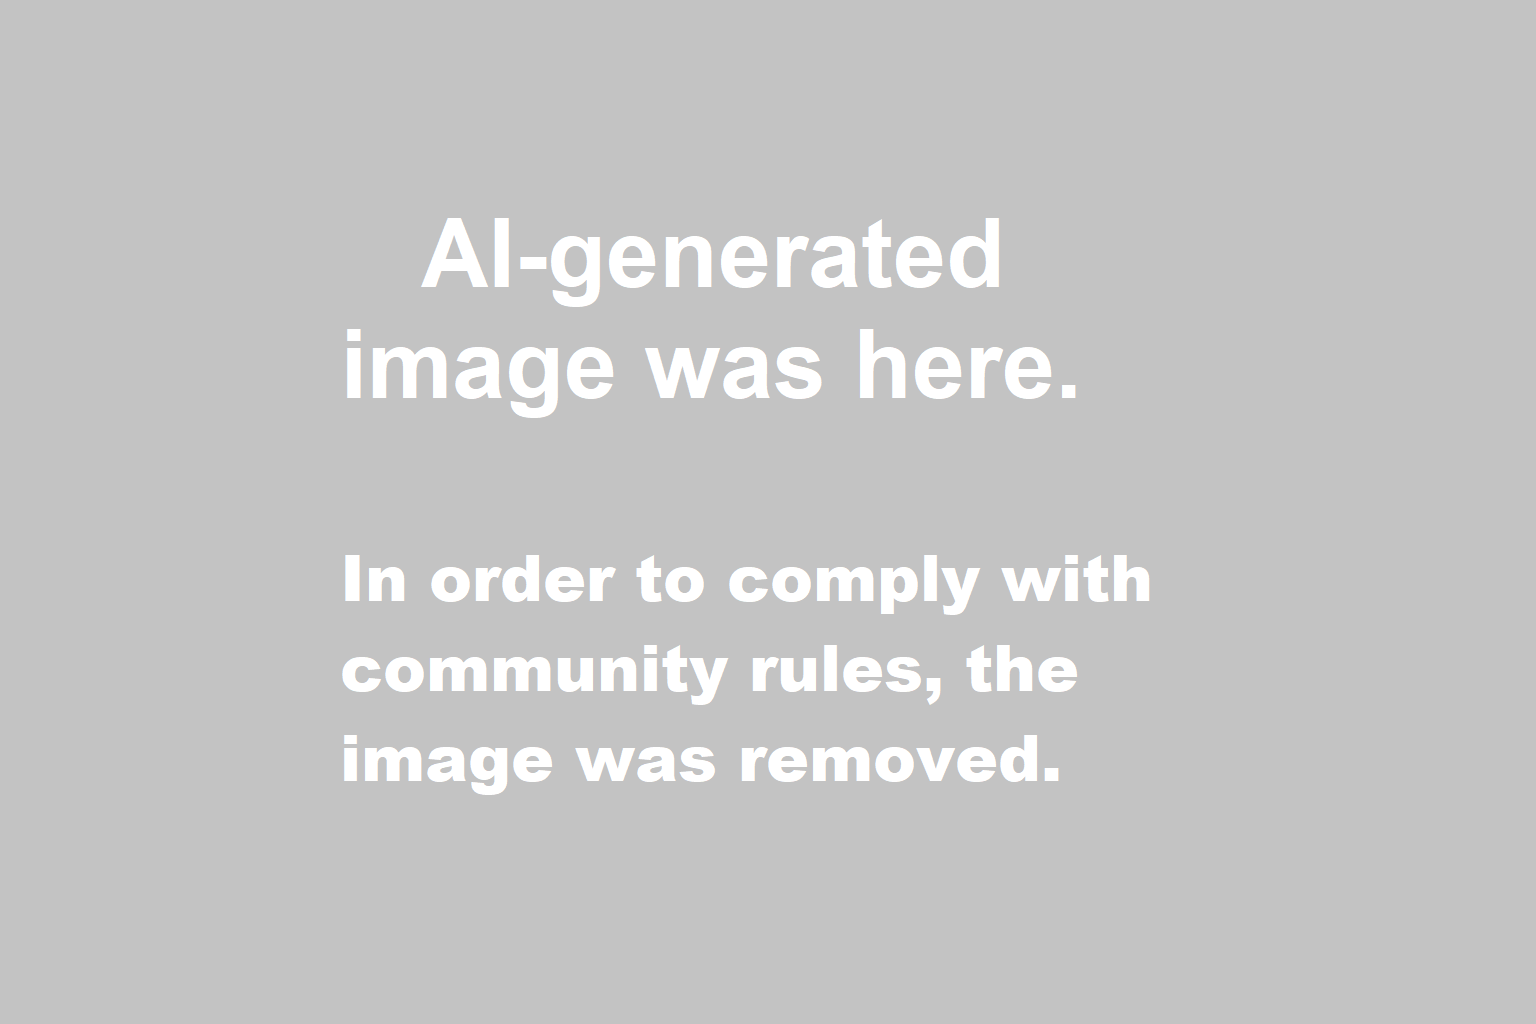
\includegraphics[width=0.45\textwidth]{images/deadShip.png}

\newpage
\enemyStatBlock{
	\enemyStatBlockHeader{\enemyKhornak}{1}{Rival}{Medium Animal}
}{
	\enemyStatBlockStats{3}{2}{0}{2}{2}{0}{26 (20–32)}{4}{0} % STR: 3+2, WIL: 2->0, HP: 26+2
}{
	\small
	\enemyStatBlockSkills[
	\enemyStatblockSkillsDeflect[2 (carapace)] \\
	\enemyStatblockSkillsMovement[25 ft., swim 30 ft.]
	\enemyStatblockSkillsSenses[10 ft. (sight)]
	\enemyStatblockSkillsPhysical[Athletics +5, Stealth +4]
	\enemyStatblockSkillsSpiritual[Perception +3, Survival +4]
	\enemyStatblockSkillsLanguages
	]
}{
	\enemyStatblockFeature{Terrifying Ambush}{At the start of each scene, each enemy who can sense the khornak must make a DC 14 Discipline test. On a failure, that enemy can’t take a fast turn this round unless they spend 2 focus.} \\
	
	\enemyStatblockFeature{Ruthless Predator}{When the khornak attacks and hits an enemy who hasn’t taken a turn yet this round, the attack deals an extra 1d8 damage.} \\
	
	\enemyStatblockFeature{Reshi-Born}{The khornak can ignore negative effects of a difficult terrain caused by plants.} \\
}{
	\enemyStatblockAction{Strike: Crushing Jaw}{Attack +5, reach 5 ft., one target. Graze: 4 (1d8) impact damage. Hit: 9 (1d8 + 5) impact damage, and the target becomes Restrained by the khornak’s jaw while the khornak remains within 5 feet of them. The khornak can spend 1 focus to also make the target Afflicted [1d4 vital] until the target regains at least 1 health.  As \iconAction{}, the target or a character who can reach them can make a DC 16 Agility or Athletics test, ending the Restrained condition on a success. While the khornak is restraining this target, the khornak can’t make another Crushing Jaw attack.}\\
	
	\enemyStatblockAction{Tail Sweep}{Attack +5, reach 5 ft., one target. The khornak can spend up to 2 focus to target that many additional targets with the same attack. Graze: 3 (1d6) impact damage. Hit: 8 (1d6 + 5) impact damage, and the target must succeed on a DC 15 Athletics test or be knocked Prone.} \\
	
	\enemyStatblockAction{Drag}{The khornak moves up to 15 feet in any direction while dragging an enemy they have Restrained behind them.}
}
\normalsize


\newpage
\section{\enemyReshiWarriorName}
\label{enemyReshiWarrior}

\enemyReshiWarrior{}s function as guards and soldiers in Reshi culture. They obey their king and priest of the island. Bold and fearless, they will never show weakness in the face of enemy.

Without access to metal ore and metallurgy, Reshi craft their weapons from shells and carapace of creatures living on their island. Carapace armor gives them intimidating look, but their weapons are even more scary - shellmaces are wooden swords overgrowing sharp-edged shells. Wounds made by this terrifying weapon bleed profusely and are very hard to heal.

\subsection{The Red Vines' Blessings}

Some of the \enemyReshiWarrior{}s worship \npcSprenVines{} - an ancient spren infecting the island with the Red Vines. In the final chapter of the story, they can be found accepting spren's blessings. At this point, they receive additional Feature - \abilityVinesName[2]:

\abilityVines[2]{}

Each \enemyReshiWarrior{} with this feature has his Strength increased by 2 (from 3 to 5). As a result, increase Physical Defense (from 14 to 16) and Health (from 24 to 26) as well. Increased Strength also affects Athletics and Heavy Weaponry skills (both to +7), attack bonus (+7) and damage (now 1d10 +7).

When \enemyReshiWarrior{} overgrown with the Red Vines dies, they will return with \abilityHuskName[2] Feature:

\abilityHusk[2]{}

They still continue to benefit from \abilityVinesName[2], but they can no longer spend their Focus. And of course - they must be defeated again...
\\

\tacticsBox{
	Strong and brutal, \enemyReshiWarrior{}s will fight to the death to protect their king. Their attacks are brutal, and they will Rend enemy's flesh to quickly remove them from combat.
}


\newpage
\enemyStatBlock{
	\enemyStatBlockHeader{\enemyReshiWarrior{}}{1}{Rival}{Medium Humanoid}
}{
	\enemyStatBlockStats{3}{1}{1}{2}{3}{1}{24 (19–29)}{4}{0}
}{
	\enemyStatBlockSkills[
	\enemyStatblockSkillsDeflect[2 (carapace)] \\
	\enemyStatblockSkillsMovement[25 ft.]
	\enemyStatblockSkillsSenses[20 ft. (sight)]
	\enemyStatblockSkillsPhysical[Athletics +5, Heavy Weaponry +5]
	\enemyStatblockSkillsCognitive[Discipline +4, Intimidation +4]
	\enemyStatblockSkillsSpiritual[Insight +4, Perception +5]
	\enemyStatblockSkillsLanguages[Reshi]
	]
}{
	\enemyStatblockFeature{Bold}{The warrior's Discipline tests have advantage. Any attempt to Intimidate the warrior has disadvantage.} \\
}{
	\enemyStatblockAction{Strike: Shellmace}{Attack +5, reach 5 ft., one target. Graze: 5 (1d10) keen damage. Hit: 10 (1d10 + 5) keen damage.}\\
	
	\enemyStatblockAction[\iconActionDouble]{Rend (Costs 2 Focus)}{Attack +5, reach 5 ft., one target. Graze: 5 (1d10) keen damage. Hit: 10 (1d10 + 5) keen damage and the target is Afflicted [1d10]. }\\
}

\newpage
\enemyStatBlock{
	\enemyStatBlockHeader{\enemyReshiWarrior{} (Enhanced)}{1}{Rival}{Medium Humanoid}
}{
	\enemyStatBlockStats{5}{1}{1}{2}{3}{1}{26 (21–31)}{4}{0}
}{
	\enemyStatBlockSkills[
	\enemyStatblockSkillsDeflect[2 (carapace)] \\
	\enemyStatblockSkillsMovement[25 ft.]
	\enemyStatblockSkillsSenses[20 ft. (sight)]
	\enemyStatblockSkillsPhysical[Athletics +7, Heavy Weaponry +7]
	\enemyStatblockSkillsCognitive[Discipline +4, Intimidation +4]
	\enemyStatblockSkillsSpiritual[Insight +4, Perception +5]
	\enemyStatblockSkillsLanguages[Reshi]
]
}{
	\enemyStatblockFeature{Bold}{The warrior's Discipline tests have advantage. Any attempt to Intimidate the warrior has disadvantage.} \\
	
	\enemyStatblockFeature{\abilityVinesName[2]}{\abilityVinesText[2]} \\
}{
	\enemyStatblockAction{Strike: Shellmace}{Attack +7, reach 5 ft., one target. Graze: 5 (1d10) keen damage. Hit: 12 (1d10 + 7) keen damage.}\\

	\enemyStatblockAction[\iconActionDouble]{Rend (Costs 2 Focus)}{Attack +7, reach 5 ft., one target. Graze: 5 (1d10) keen damage. Hit: 12 (1d10 + 7) keen damage and the target is Afflicted [1d10]. }\\
}


\newpage
\enemyStatBlock{
	\enemyStatBlockHeader{Reanimated \enemyReshiWarrior{}}{1}{Rival}{Medium Humanoid}
}{
	\enemyStatBlockStats{5}{1}{0}{0}{3}{1}{26 (21–31)}{0}{0}
}{
	\enemyStatBlockSkills[
	\enemyStatblockSkillsDeflect[2 (carapace)] \\
	\enemyStatblockSkillsMovement[25 ft.]
	\enemyStatblockSkillsSenses[20 ft. (sight)]
	\enemyStatblockSkillsPhysical[Athletics +7, Heavy Weaponry +7]
	\enemyStatblockSkillsCognitive[Discipline +4, Intimidation +4]
	\enemyStatblockSkillsSpiritual[Insight +4, Perception +5]
	\enemyStatblockSkillsLanguages[Reshi]
	]
}{
	\enemyStatblockFeature{Bold}{The warrior's Discipline tests have advantage. Any attempt to Intimidate the warrior has disadvantage.} \\
	
	\enemyStatblockFeature{\abilityVinesName[2]}{\abilityVinesText[2]} \\
	
	\enemyStatblockFeature{\abilityHuskName[2]}{\abilityHuskText[2]} \\
}{
	\enemyStatblockAction{Strike: Shellmace}{Attack +7, reach 5 ft., one target. Hit: 12 (1d10 + 7) keen damage.}\\
}
\newpage
\section{\enemyRogueShardbearerName}
\label{enemyRogueShardbearer}

Most of the Shardblades are bonded to Shardbearers appointed by rulers and their blades are carefully watched. Those wonders can change the tide of battle and rewrite realms' history and everyone is carefully tracking them.

Most, but not all. Some fell into a wrong hands of people who prefer operating from the shadows: thieves, assassins or crime lords. They keep information about the blade hidden and their enemies can only glimpse the flash of them right before their demise.

Fighting \enemyRogueShardbearer{} is a difficult task - their weapon is deadly and they will not hesitate to play dirty. However, the reward is worth it, as the \lootRogueShardblade{} will belong to anyone who is skilled or lucky enough to survive such fight.
\\

\tacticsBox{
	\enemyRogueShardbearer{} approaches carefully to the fight. While their weapon is deadly, they are not invincible. They will dodge, hide, use dirty tricks to ensure they will live long enough to make the cut with their Shardblade.
}

\vspace{1cm}
\includeCreditedGraphics{width=0.40\textwidth}{images/rogueShardbearer.png}{AI}

\newpage
\enemyStatBlock{
	\enemyStatBlockHeader{\enemyRogueShardbearer{}}{1}{Boss}{Medium Humanoid}
}{
	\enemyStatBlockStats{3}{2}{5}{2}{2}{4}{55 (45–65)}{6}{0}
}{
	\small
	\enemyStatBlockSkills[
	\enemyStatblockSkillsDeflect[1 (leather)] \\
	\enemyStatblockSkillsMovement[25 ft.]
	\enemyStatblockSkillsSenses[20 ft. (sight)]
	\enemyStatblockSkillsPhysical[Heavy Weaponry +6, Light Weaponry +5, Athletics +5]
	\enemyStatblockSkillsCognitive[Deduction +8, Discipline +6, Intimidation +6]
	\enemyStatblockSkillsSpiritual[Deception +7, Leadership +7, Perception +5, Persuasion +6]
	\enemyStatblockSkillsLanguages[defined by culture]
	]
}{
	\enemyStatblockFeatureBoss{} \\
}{
	\enemyStatblockAction{Strike: Knife}{Attack +5, reach 5 ft, one target. Graze: 2 (1d4) keen damage. Hit: 8 (1d4 + 6) keen damage plus 7 (2d6) vital damage, and the target must succeed on a DC 16 Athletics test or become \exhausted{}.}\\
	
	\enemyStatblockAction{Strike: Shardblade}{Attack +6, reach 5 ft, one target. Graze: 9 (2d8) spirit damage. Hit: 15 (2d8 + 6) spirit damage.}\\

	\enemyStatblockAction{Flash Fabrial (Costs 1 Focus)}{The rogue activates a fabrial that emits a piercing light from its gemstone. Each character within 10 feet of the rogue must succeed on a DC 15 Discipline test or become Disoriented until the end of the rogue’s next turn.}\\
	
	\enemyStatblockAction{Subdue}{The rogue menaces a foe, making an opposed Intimidation test against the target’s Discipline. If the rogue succeeds, the target loses 1d4 focus and gains a disadvantage on tests against the rogue until the end of the rogue’s next turn.}\\
	
	\enemyStatblockAction{Firemoss}{The rogue grinds firemoss and inhales the smoke, regaining 6 focus}\\
}

\newpage
\section{Reanimated Husks}

Despite Reanimated Husks term can cover many enemies, they all share some common elements: they all have been alive once, but after their demise they were reanimated back to life as and undead puppets controlled by the Red Vines.

Due to the Red Vines affecting animated body, all of them receive Strength (and all skills, attributes and attacks affected by it) boost with the feature of \abilityVinesName{}:

\abilityVines{}

Since they are already dead, they also benefit from \abilityHuskName{} Feature:

\abilityHusk{}

As a result, the Reanimated Husk is a strong enemy focusing on brutal attacks, but it lacks finesse of a trained warrior - it cannot Graze and use its Focus abilities.

Since they are not fully alive, killing them doesn't need to end their existence. Some parts of the Husk's body can still contain enough Red Vines to continue fighting as \enemyReanimatedRemains{}. Those are severed limbs or other body parts that are puppeteered back into the fight.

In case of all living creatures, the bigger they are, the bigger the influence of the Red Vines. Both \abilityVinesName{} and \abilityHuskName{} scale with the size of the creature affected by them: \\

\begin{tabular}{c c c}
	Size 		& Scale & Ability Example \\ \hline
	Small 		& 1 & \abilityVinesName[1] \\
	Medium 		& 2 & \abilityVinesName[2] \\
	Large 		& 3 & \abilityVinesName[3] \\
	Huge 		& 4 & \abilityVinesName[4] \\
	Gargantuan 	& 5 & \abilityVinesName[5] \\
\end{tabular}

\tacticsBox{
	All Reanimated Husks attack whoever they can, and they never stop. They don't care about pain or death - they are already dead. All they want is to tear flesh, draw blood and spread the Red Vines' infestation.
}



\newpage
\section{\enemyReanimatedRemainsName{}}
\label{enemyReanimatedRemains}

\enemyStatBlock{
	\enemyStatBlockHeader{\enemyReanimatedRemains{}}{1}{Minion}{Small Undead Plant}
}{
	\enemyStatBlockStats{3}{1}{0}{0}{2}{0}{10 (8–12)}{0}{0} % STR: 2+1, WIL: 1->0, HP: 9+1
}{
	\enemyStatBlockSkills[
	\enemyStatblockSkillsMovement[25 ft.]
	\enemyStatblockSkillsSenses[10 ft. (touch)]
	\enemyStatblockSkillsPhysical[Stealth +3]
	\enemyStatblockSkillsSpiritual[Survival +4]
	\enemyStatblockSkillsLanguages
	]
}{
	\enemyStatblockFeature{\abilityVinesName[1]}{\abilityVinesText[1]} \\
	
	\enemyStatblockFeature{\abilityHuskName[1]}{\abilityHuskText[1]} \\
	
	\enemyStatblockFeatureMinion \\
}{
	\enemyStatblockAction{Strike: Slam}{Attack +3, reach 5 ft., one target. Hit: 5 (1d4 + 3) keen damage.}\\
}


\vspace{0.75cm}
{\hfill \includeCreditedGraphics{width=0.40\textwidth}{images/reanimatedRemains.png}{AI} \hfill}


\newpage
\section{\enemyReanimatedAxehoundName}
\label{enemyReanimatedAxehound}

\enemyStatBlock{
	\enemyStatBlockHeader{\enemyReanimatedAxehound}{1}{Minion}{Small Undead Animal Plant}
}{
	\enemyStatBlockStats{3}{2}{0}{0}{3}{0}{13 (10-16)}{0}{0} % STR: 2+1, HP: 12+1
}{
	\enemyStatBlockSkills[
	\enemyStatblockSkillsMovement[40 ft.]\\
	\enemyStatblockSkillsSenses[40 ft. (smell)]
	\enemyStatblockSkillsPhysical[Agility +4, Athletics +5, Stealth +3]
	\enemyStatblockSkillsSpiritual[Perception +5, Survival +4]
	\enemyStatblockSkillsLanguages
	]
}{
	\enemyStatblockFeature{Enhanced Senses}{The axehound gains an advantage on non-attack tests that rely on smell.} \\
	
	\enemyStatblockFeature{Herdazian Breed}{The axehound gains an advantage on Survival tests.} \\	
	
	\enemyStatblockFeature{\abilityVinesName[1]}{\abilityVinesText[1]} \\
	
	\enemyStatblockFeature{\abilityHuskName[1]}{\abilityHuskText[1]} \\
	
	\enemyStatblockFeatureMinion{}
}{
	\enemyStatblockAction{Strike: Bite}{Attack +5, reach 5 ft., one target. Hit: 7 (1d4 + 5) keen damage.}\\
	
	\enemyStatblockAction[\iconFreeAction]{Pack Instincts}{While within 5 feet of an ally, the axehound can use the Gain Advantage action as \iconFreeAction{}.} \\
	
	\enemyStatblockAction[\iconReaction]{On the Hunt}{After an enemy within 30 feet of the axehound falls Prone, the axehound moves up to 15 feet toward them.}
}

\newpage
\section{\enemyReanimatedKhornakName}
\label{enemyReanimatedKhornak}

\enemyStatBlock{
	\enemyStatBlockHeader{\enemyReanimatedKhornak}{1}{Rival}{Medium Undead Animal Plant}
}{
	\enemyStatBlockStats{5}{2}{0}{0}{2}{0}{28 (22–34)}{0}{0} % STR: 3+2, WIL: 2->0, HP: 26+2
}{
	\small
	\enemyStatBlockSkills[
	\enemyStatblockSkillsDeflect[2 (carapace)] \\
	\enemyStatblockSkillsMovement[25 ft., swim 30 ft.]
	\enemyStatblockSkillsSenses[10 ft. (sight)]
	\enemyStatblockSkillsPhysical[Athletics +7, Stealth +4]
	\enemyStatblockSkillsSpiritual[Perception +3, Survival +4]
	]
}{
	\enemyStatblockFeature{Terrifying Ambush}{At the start of each scene, each enemy who can sense the khornak must make a DC 14 Discipline test. On a failure, that enemy can’t take a fast turn this round unless they spend 2 focus.} \\
	
	\enemyStatblockFeature{Ruthless Predator}{When the khornak attacks and hits an enemy who hasn’t taken a turn yet this round, the attack deals an extra 1d8 damage.} \\
	
	\enemyStatblockFeature{\abilityVinesName[2]}{\abilityVinesTextShort[2]} \\
	
	\enemyStatblockFeature{\abilityHuskName[2]}{\abilityHuskText[2]} 
}{
	\enemyStatblockAction{Strike: Crushing Jaw}{Attack +5, reach 5 ft., one target. Hit: 9 (1d8 + 5) impact damage, and the target becomes Restrained while the khornak remains within 5 feet of them. As \iconAction{}, the target or a character who can reach them can make a DC 16 Agility or Athletics test, ending the Restrained condition on a success. While the khornak is restraining this target, the khornak can’t make another Crushing Jaw attack.}\\
	
	\enemyStatblockAction{Tail Sweep}{Attack +5, reach 5 ft., one target. Hit: 8 (1d6 + 5) impact damage, and the target must succeed on a DC 15 Athletics test or be knocked Prone.} \\
	
	\enemyStatblockAction{Drag}{The khornak moves up to 15 feet in any direction while dragging an enemy they have Restrained behind them.}
}
\normalsize


\newpage
\section{\enemyReanimatedWhitespineName{}}
\label{enemyReanimatedWhitespine}

\enemyStatBlock{
	\enemyStatBlockHeader{\enemyReanimatedWhitespine}{2}{Rival}{Large Undead Animal Plant}
}{
	\enemyStatBlockStats{7}{3}{0}{0}{4}{0}{48 (39–56)}{4}{0} % STR: 4+3, WIL: 2->0, HP 42+3+3
}{
	\enemyStatBlockSkills[
	\enemyStatblockSkillsDeflect[1 (carapace)]\\
	\enemyStatblockSkillsMovement[60 ft.]
	\enemyStatblockSkillsSenses[40 ft. (smell)]
	\enemyStatblockSkillsPhysical[\small Agility +6, Athletics +10, Stealth +6 \normalsize]
	\enemyStatblockSkillsCognitive[Intimidation +3]
	\enemyStatblockSkillsSpiritual[Perception +6, Survival +6]
	\enemyStatblockSkillsLanguages
	]
}{
	\enemyStatblockFeature{Enhanced Senses}{The whitespine gains an advantage on non-attack tests that rely on smell.} \\
	
	\enemyStatblockFeature{Spined Carapace}{After an enemy within 5 feet of the whitespine grazes them with a weapon attack, that enemy takes 3 (1d6) keen damage} \\
	
	\enemyStatblockFeature{Reshi-Born}{The whitespine can ignore negative effects of a difficult terrain caused by plants.} \\
	
	\enemyStatblockFeature{\abilityVinesName[3]}{\abilityVinesTextShort[3]} \\
	
	\enemyStatblockFeature{\abilityHuskName[3]}{\abilityHuskText[3]} \\
	
}{
	\enemyStatblockAction{Strike: Claws}{Attack +10, reach 5 ft., one target. Hit: 13 (1d6 + 10) keen damage.} \\
	
	\enemyStatblockAction{Goring Tusks}{Attack +10, reach 5 ft., one target. Hit: 15 (1d10 + 10) impact damage. If the whitespine hits with this attack immediately after moving at least 15 feet, the target takes an extra 5 (1d10) impact damage and must succeed on a DC 17 Athletics test or be knocked Prone.}\\ 
}


\newpage
\section{\enemyReanimatedPersonName}
\label{enemyReanimatedPerson}

The stat block below assumes the person was \textbf{Expert Citizen} \textit(see \bookWorldGuide{}) before death and reanimation. For other cases, please adjust other stat blocks. \\

 
\enemyStatBlock{
	\enemyStatBlockHeader{\enemyReanimatedPerson{}}{1}{Rival}{Medium Undead Humanoid Plant}
}{
	\enemyStatBlockStats{3}{1}{0}{0}{2}{1}{20 (17–23)}{0}{0} % STR: 1+2, INT: 1->0 WIL: 2->0, HP: 18+2
}{
	\enemyStatBlockSkills[
	\enemyStatblockSkillsMovement[25 ft.] \\
	\enemyStatblockSkillsSenses[10 ft. (sight)]
	\enemyStatblockSkillsPhysical[Agility +2, Athletics +4]
	\enemyStatblockSkillsSpiritual[Insight +4, Perception +4]
	\enemyStatblockSkillsLanguages
	]
}{
	\enemyStatblockFeature{\abilityVinesName[2]}{\abilityVinesTextShort[2]} \\
	
	\enemyStatblockFeature{\abilityHuskName[2]}{\abilityHuskText[2]} \\
}{
	\enemyStatblockAction{Strike: Unarmed Attack}{Attack +4, reach 5 ft., one target. Hit: 6 (1d4 + 4) impact damage.}\\
}

\vspace{0.35cm}
{\hfill \includeCreditedGraphics{width=0.40\textwidth}{images/reanimatedWhitespine.png}{AI} \hfill}
\newpage
\section{\enemyVineMonsterName}
\label{enemyVineMonster}

Empowered by the influence of \npcSprenVines{} and invigorated by blood sacrifices, the Red Vines can grow into \enemyVineMonster{}, making them even more deadly threat.

Even if overgrown, \enemyVineMonster{} is still the rockbud vine. It is nearly indistinguishable from other vines growing in the area and can easily surprise inattentive adventurers. Its vines have quite a reach, but luckily the plant itself cannot move.

Growing from the Red Vines, \enemyVineMonster{} can enhance bodies of the fallen creatures and reanimate them as \enemyReanimatedRemains{}. At first the corpse must be in close range of the plant, but after some time the puppet can detach from the main plant and roam free by itself.

Sustaining on blood from sacrifices and its victims, the plant is very vital and quickly regenerates, but it is also vulnerable to fire.

\tacticsBox{
	\enemyVineMonster{} waits patiently for its prey to come close enough. When the time is right, it strikes with its Vine Whip, hopefully restraining the unsuspecting foe. After that it aims to crush the body of the victim, drink its blood and Puppeteer the remains in hopes to lure another victim nearby. 
}


{\hfill \includeCreditedGraphics{width=0.35\textwidth}{images/vineMonster.png}{AI} \hfill}

\newpage
\enemyStatBlock{
	\enemyStatBlockHeader{\enemyVineMonster{}}{1}{Rival}{Medium Plant}
}{
	\enemyStatBlockStats{1}{3}{1}{2}{2}{1}{33 (28–38)}{4}{0}
}{
	\enemyStatBlockSkills[
	\enemyStatblockSkillsMovement[0 ft.]\\
	\enemyStatblockSkillsSenses[10 ft. (touch)]
	\enemyStatblockSkillsPhysical[Agility +5, Stealth +5]
	\enemyStatblockSkillsSpiritual[Survival +4]
	\enemyStatblockSkillsLanguages
	]
}{
	\enemyStatblockFeature{Flammable}{This creature takes double energy damage from fire sources.}\\
	
	\enemyStatblockFeature{Rugged Camouflage}{An undetected vine gains an advantage on attack tests. While the vine is motionless, it's almost indistinguishable from a normal vine, requiring a successful DC 15 Survival test to identify it. This test gains a disadvantage when the vine is in cover or in an area where the other character’s primary sense is obscured.} \\
}{
	\enemyStatblockAction{Strike: Vine Whip}{Attack +5, reach 25 ft., one target. Graze: 3 (1d6) keen damage. Hit: 6 (1d6 + 3) keen damage and the vine can spend 1 focus to wrap around the target. If it does, the target becomes \restrained{}. As \iconAction{}, the Restrained target or a character within 5 ft. can make \skillCheck{15}{Athletics} to release the target on success.}\\
	
	\enemyStatblockAction{Constrict}{The vine attempts to crush an enemy Restrained by it. That enemy must pass \skillCheck{15}{Athletics}. The vine deals 3 (1d6) impact damage to them on failure and heals for the same amount.}\\
	
	\enemyStatblockAction{Puppeteer Remains (Costs 1 Focus)}{The vine animates a corpse within 20 ft. range, turning it into \enemyReanimatedRemains{} for as long it stays within the range. Unless slain or disjointed from the vine, the puppet will gain full autonomy after 1 hour.}
}


\newpage
\section{\enemyVineAbominationName}
\label{enemyVineAbomination}

Given enough time and blood, \enemyVineMonster{} will eventually grow into \enemyVineAbomination{} - huge mass of bones, corpses and Red Vines dripping blood onto the battlefield.

Those horrors are often found nearby sacrificial altars, where they are offered continuous supply of sustenance.

Growing out of proportions, those grotesque plants are impossible to miss and they have much harder time blending into the surrounding than its younger and less developed forms. However, they are strong enough to slowly pull themselves closer to their enemies, increasing reach of their attacks.

\tacticsBox{
	Grown on blood, \enemyVineAbomination{} has always thirst for more. It will Vine Whip anyone who is close enough in order to Constrict them later. If enemies are out of range, it will Hurl Remains onto them, spawning allies in the process. When overwhelmed by foes, \enemyVineAbomination{} will use Tripping Whip and Puppeteer Corpse to even the odds.
}

\vspace{1cm}
{\hfill \includeCreditedGraphics{width=0.40\textwidth}{images/vineAbomination.png}{AI} \hfill}

\newpage
\enemyStatBlock{
	\enemyStatBlockHeader{\enemyVineAbomination{}}{2}{Boss}{Large Plant}
}{
	\enemyStatBlockStats{3}{5}{2}{3}{4}{2}{100 (75–125)}{5}{0} 
}{
\small
	\enemyStatBlockSkills[
	\enemyStatblockSkillsMovement[10 ft.]\\
	\enemyStatblockSkillsSenses[20 ft. (touch)]
	\enemyStatblockSkillsPhysical[Agility +8, Stealth +8]
	\enemyStatblockSkillsSpiritual[Survival +6]
	\enemyStatblockSkillsLanguages
	]
}{
	\enemyStatblockFeature{Flammable}{This creature takes double energy damage from fire sources.}\\
	
	\enemyStatblockFeatureBoss{}\\
}{
	\enemyStatblockAction{Strike: Vine Whip}{Attack +8, reach 25 ft., one target. Graze: 3 (1d6) keen damage. Hit: 11 (1d6 + 8) keen damage and the vine can spend 1 focus to wrap around the target. If it does, the target becomes \restrained{}. As \iconAction{}, the Restrained target or a character within 5 ft. can make \skillCheck{18}{Athletics} to release the target on success.}\\
	
	\enemyStatblockAction{Strike: Hurl Remains}{Attack +8, range 30/120 ft., one target. Graze: 3 (1d6) impact damage. Hit: 11 (1d6 + 8) impact damage. Spawn \enemyReanimatedRemains{} within 5 ft. from the target \textit{(even if the attack did not hit).}} \\
	
	\enemyStatblockAction{Constrict}{The vine attempts to crush an enemy Restrained by it. That enemy must pass \skillCheck{18}{Athletics}. The vine deals 3 (1d6) impact damage to them on failure and heals for the same amount.}\\
	
	\enemyStatblockAction{Tripping Whip (Costs 1 Focus)}{An enemy within 25 ft. must pass \skillCheck{18}{Agility} or falls Prone.}\\
	
	\enemyStatblockAction{Puppeteer Corpse (Costs 1 Focus)}{The vine animates a corpse within 20 ft. range, giving it \abilityVinesName{} and \abilityHuskName{} for as long it stays within the range. Unless slain or disjointed from the vine, the puppet will gain full autonomy after 1 hour.} \\
	
	\enemyStatblockAction[\iconActionDouble]{Drink Blood}{The vine drinks blood from a nearby source, regaining 5 focus and 5 health.}
}
\normalsize











	\chapter{Appendix \thechapter{}: Items}
\label{chap:items}

Following unique items can be found or earned by the characters during the adventure:

\section{\lootPerfectGemstoneName}

Gemstone perfectly cut into a round sphere. It can trap and hold a single spren forever.

In order to entice the spren into entering the gemstone, it must be exposed to something it is familiar with. As \iconAction{} a character holding the gemstone may produce a statement or present a behavior that aligns with spren's nature or philosophy. Any insincere attempts must be preceded with a successful \skillCheck{20}{Deception}

\scriptedOption{Success!}{
	If the spren approves of the statement or particular action, add 1 to the capture track.
}

\scriptedOption{Failure!}{
	If the spren does not agree with the statement or behavior, or if the Deception check failed, subtract 1 from the capture track.
}

\scriptedOption{Captured!}{
	Once the capture track reaches level of 3, the spren created enough Connection with the character to be lured into the gem. It cannot leave it unless the gemstone is shattered.
}

\section{\lootRogueShardbladeName}

A Shardblade in possession of criminal underworld. Few people know of its existence. A character claiming this item will not be pushed into the politics of the nearby realms. The Blade follows all standard Shardblade rules (see \handbook{}).\\

\noindent
% \textbf{Type:} Shardblade \\
% \textbf{Skill:} Heavy Weaponry\\
% \textbf{Damage:} 2d8 spirit \\
% \textbf{Range:} Melee\\
% \textbf{Expertise:} loses Dangerous trait\\
% \textbf{Traits and Rules:} Dangerous, Deadly, Unique: Summoning/Dismissing Spiritual Injury


\section{\lootSprenDaggerName}

An ancient Reshi dagger, forged with Reshi songs in order to fight hostile spren. Upon contact with any cognitive being, the dagger releases an enormous amount of energy, annihilating both the target and the wielder.

\section{\lootTorchShortName}

Short torch, made from metal. It is decorated with twisty, sinuous patterns, similar to vine stalks - now rusty and crumbling from the age. \\

\noindent
\textbf{Type:} Mace \\
\textbf{Skill:} Light Weaponry\\
\textbf{Damage:} 1d4 impact \\
\textbf{Range:} Melee\\
\textbf{Expertise:} gains Momentum trait\\
\textbf{Traits and Rules:} Extinguishable, Flaming [1d6] \textit{(see Below)}


\section{\lootTorchLongName}

An old and rusty torch with a 6 ft. shaft. Whole torch is made of metal decorated with twisty, sinuous patterns, similar to vine stalks. \\

\noindent
\textbf{Type:} Longspear \\
\textbf{Skill:} Heavy Weaponry\\
\textbf{Damage:} 1d4 impact \\
\textbf{Range:} Melee [+5]\\
\textbf{Expertise:} gains Defensive trait\\
\textbf{Traits and Rules:} Two-Handed, Extinguishable, Flaming [1d8] \textit{(see Below)} \\ \\

\noindent \Large \textbf{Unique Torch Traits} \normalsize \\


\scriptedOption{Extinguishable}{
	The GM can spend \iconComp{} from an attack with this weapon to extinguish it at the end of turn. As long as this weapon is extinguished, it looses Flaming trait. As \iconAction{}, a character may light the torch again to restore the trait.
}

\scriptedOption{Flaming [N]}{
	On hit, this weapon deals additional N energy damage from fire.
}



	\chapter{Appendix \thechapter{}: Example Character Sheets}
\label{chap:exampleSheets}

If you don't want to spend time on your own character's creation, here you can find some example character sheets prepared for this adventure. You can grab the one you like and just start playing. If you feel like it, you can modify your character's appearance, motivation or other details, but overall the sheets are ready to play.

In here you can find:
\begin{itemize}
	\item Zetha-daughter-Thala, herbalist \\ \textit{(Human Shin, Scholar - Surgeon)}
	\item Szar-son-son-Taszar, bodyguard \\ \textit{(Human Shin, Warrior - Soldier)}
	\item Dyrlis, ship captain \\ \textit{(Human Iriali, Leader - Officer)}
	\item Vairsh of the royal family \\ \textit{(Human Reshi, Envoy - Diplomat)}
	\item Lirah, the troublemaker \\ \textit{(Human Riran, Hunter - Assassin)}
	\item Eldrin, ship worker \\ \textit{(Singer Iriali, Agent)}
\end{itemize}
\newpage 

If none of those align to your vision of the character you want to play, make your own one! It's super easy and fun! Grab one empty character sheet, follow instructions from \handbook{} or from other sources you prefer and you will have your own hero in no time!

You can find empty character sheet template in here: \\

\href{https://www.brotherwisegames.com/stormlight-sheet}{www.brotherwisegames.com/stormlight-sheet}
\newpage

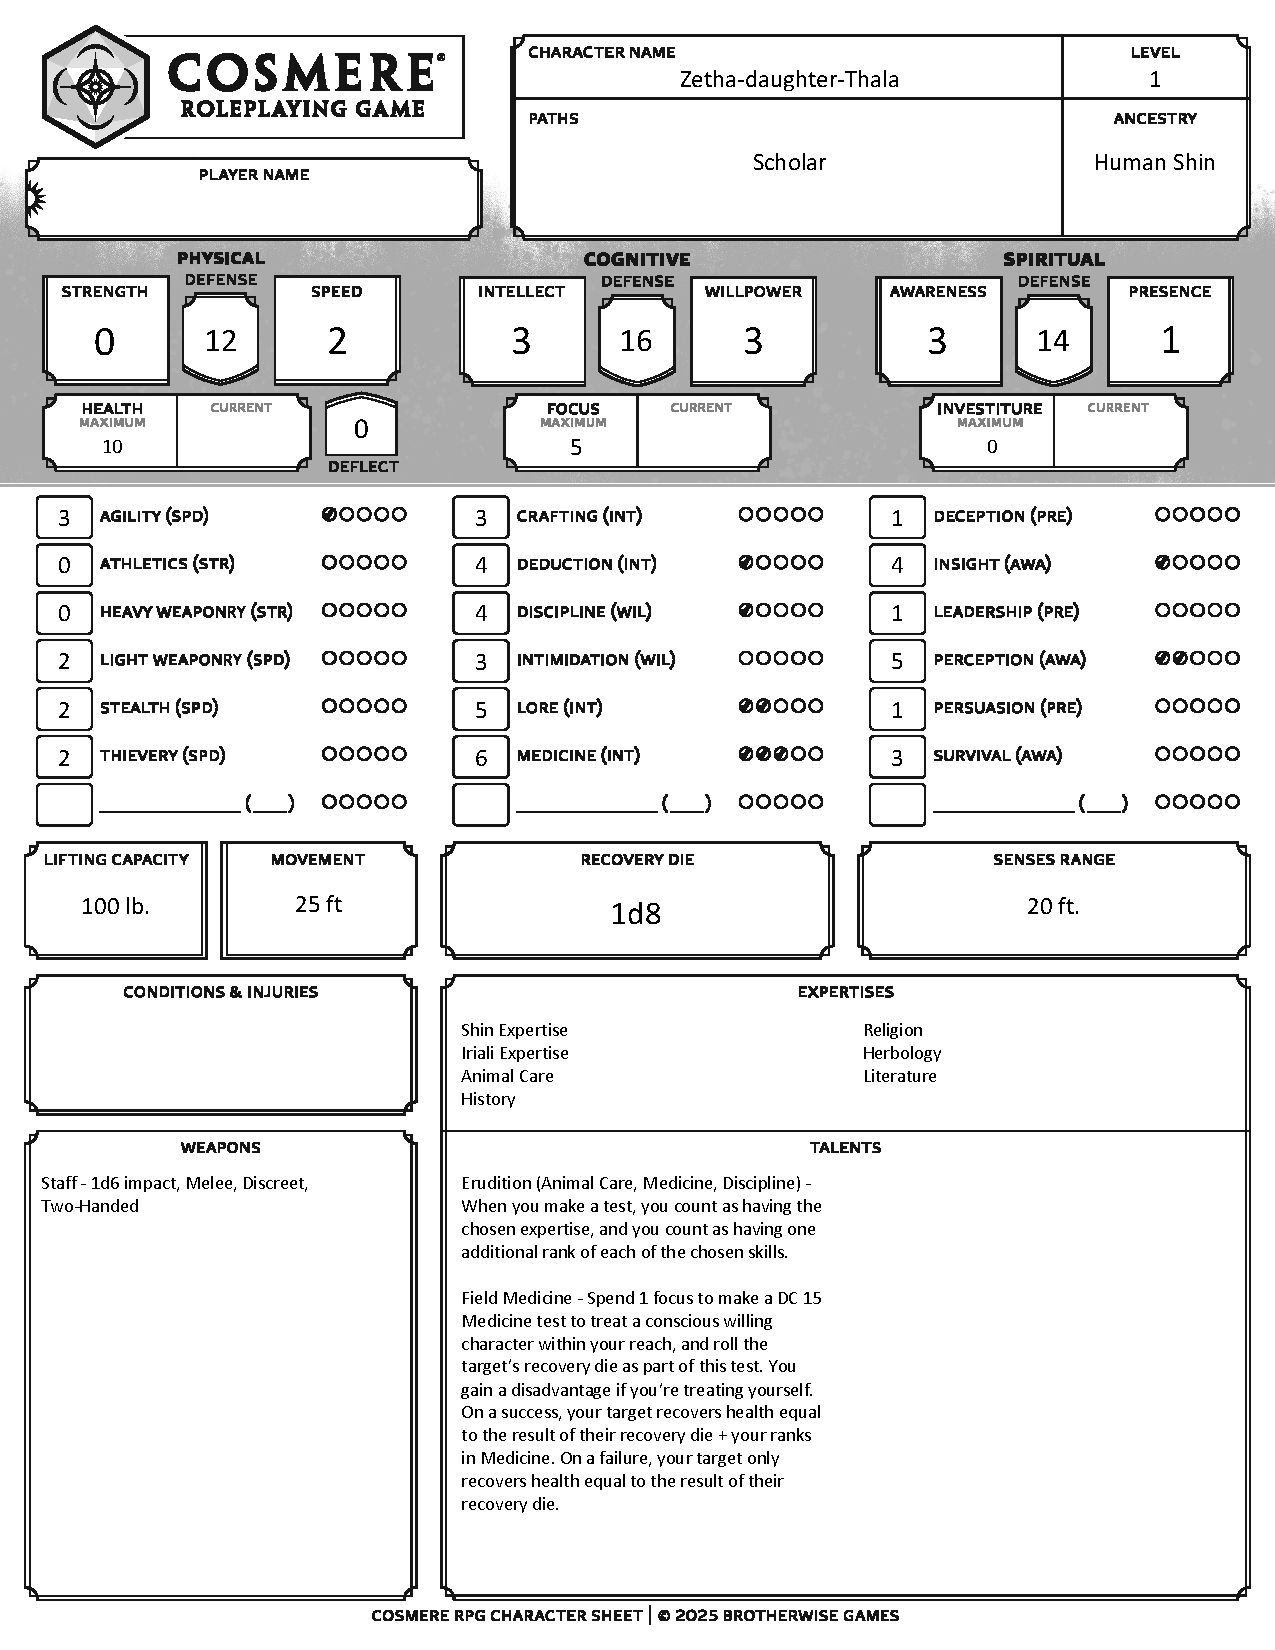
\includepdf[pages=-]{appendices/exampleSheets/example_sheet_shin_scholar_print.pdf}
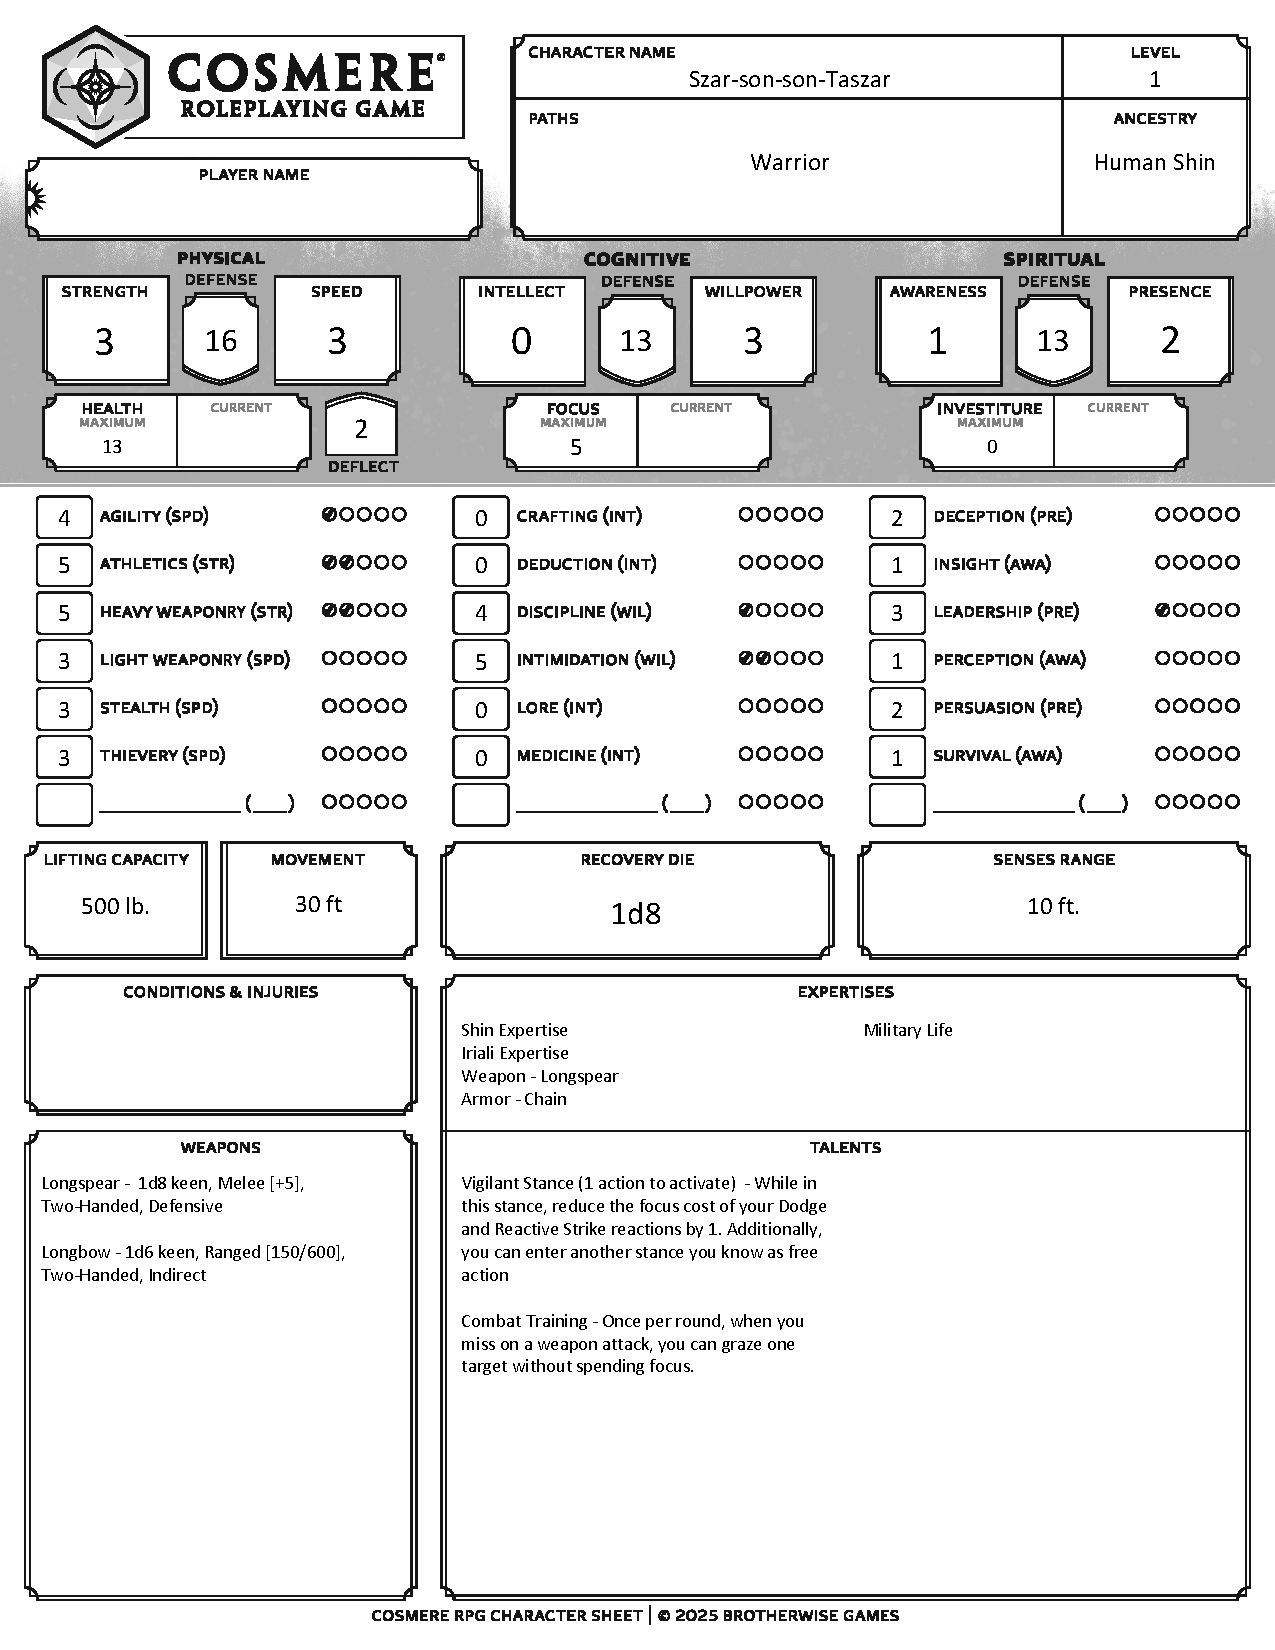
\includepdf[pages=-]{appendices/exampleSheets/example_sheet_shin_warrior_print.pdf}
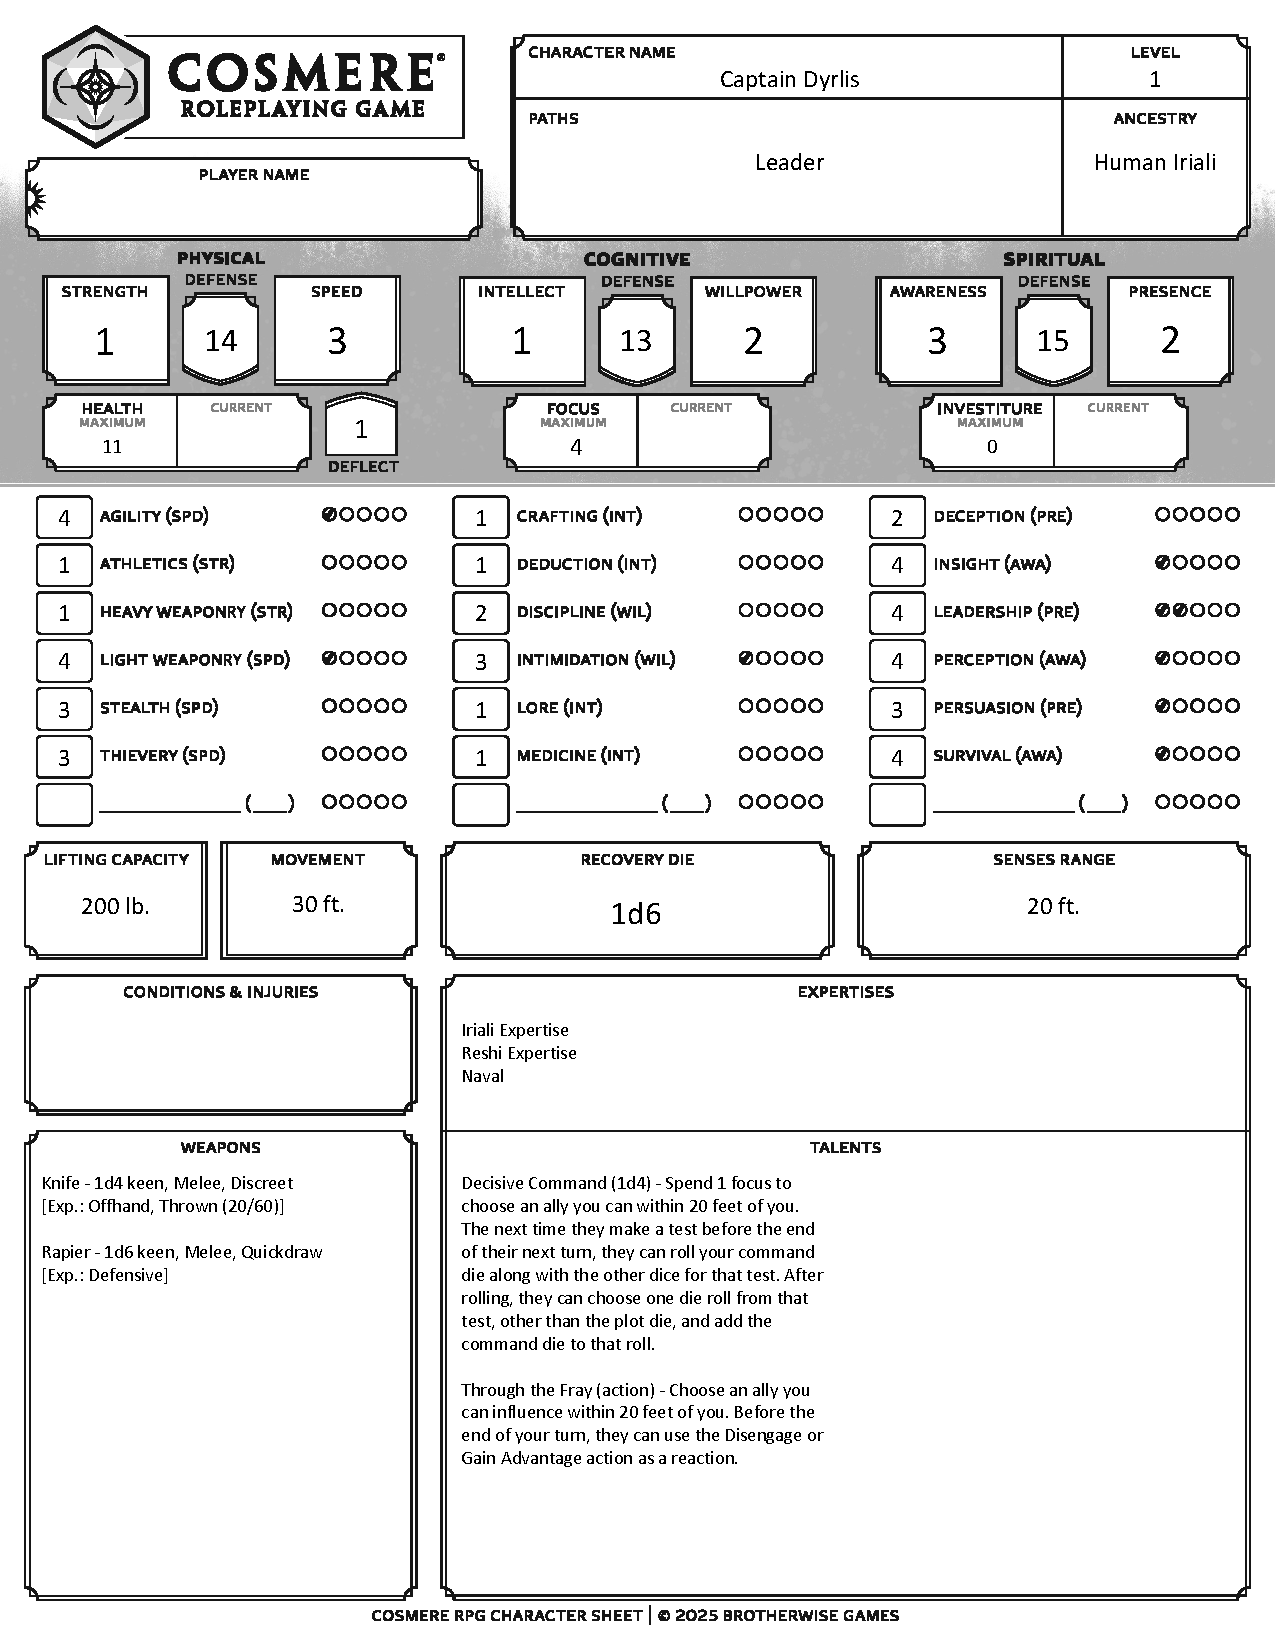
\includepdf[pages=-]{appendices/exampleSheets/example_sheet_iriali_leader_print.pdf}
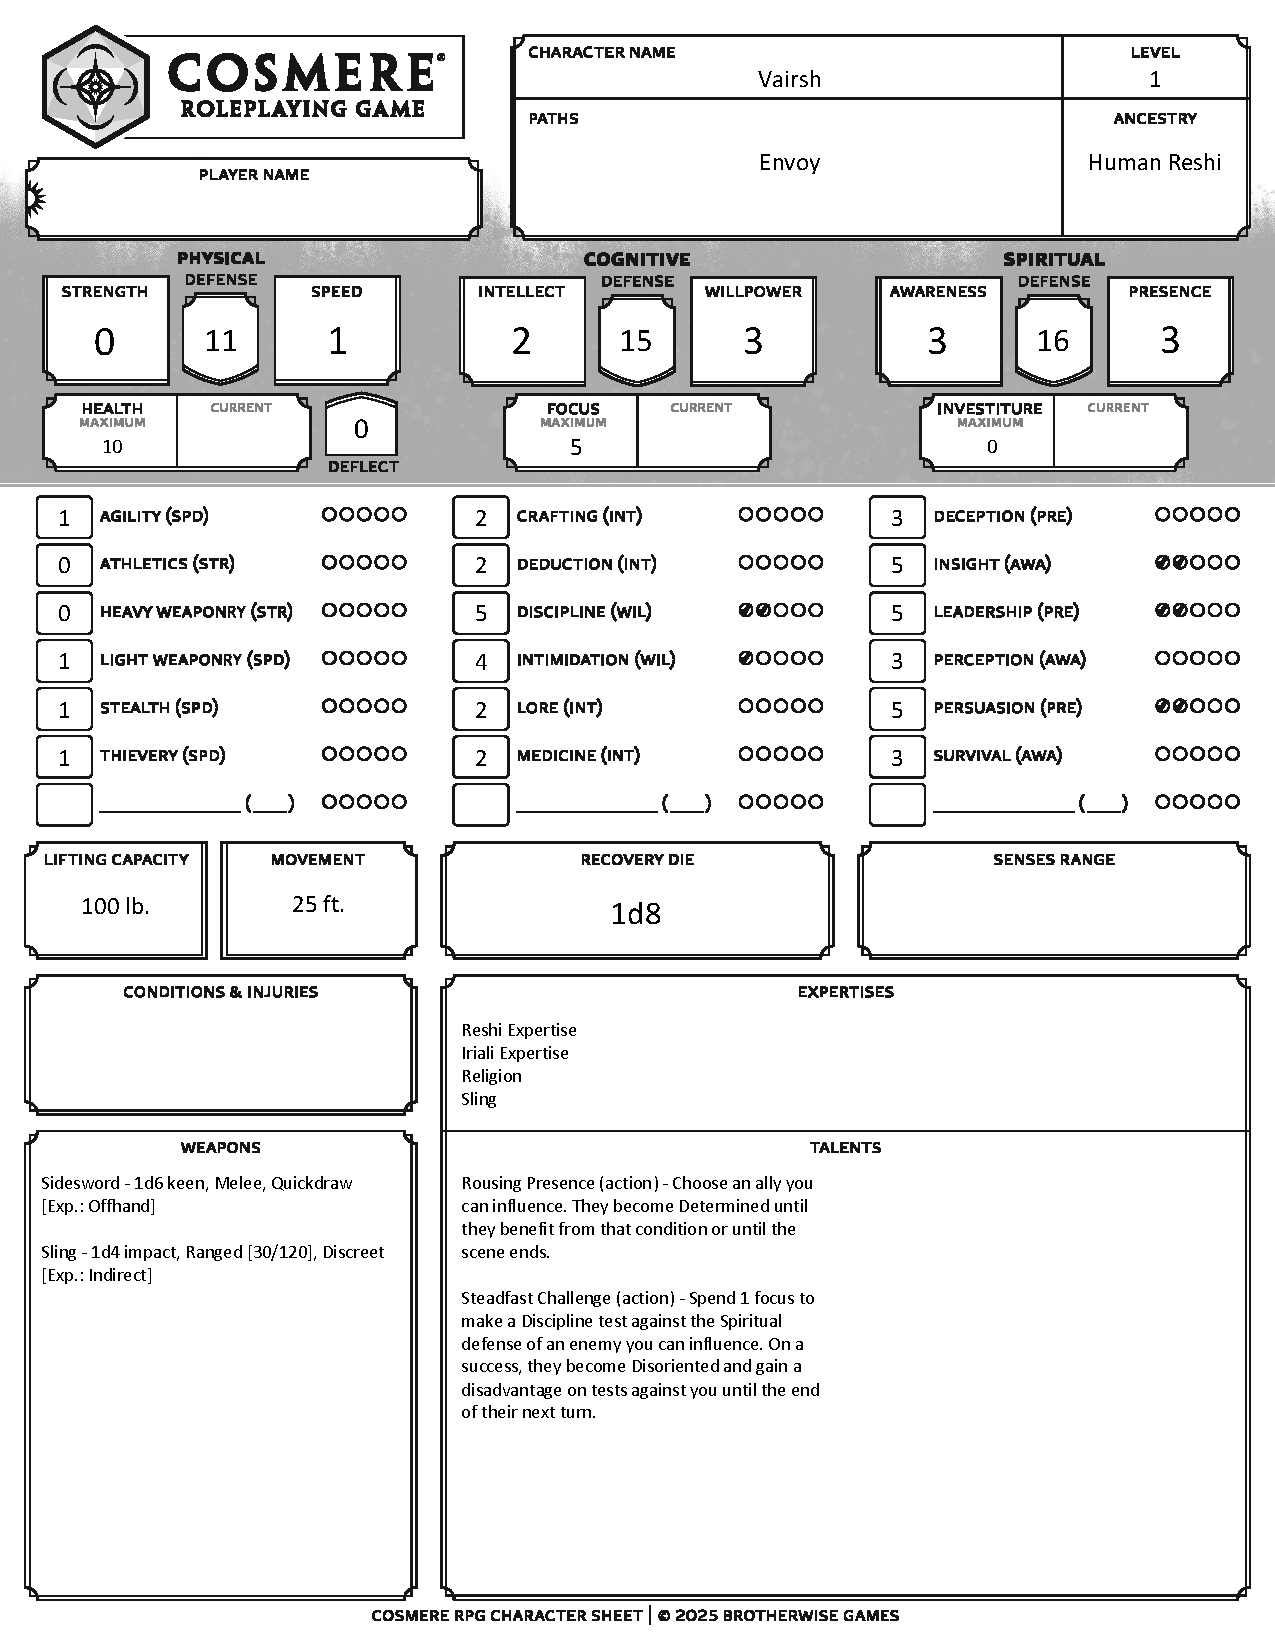
\includepdf[pages=-]{appendices/exampleSheets/example_sheet_reshi_envoy_print.pdf}
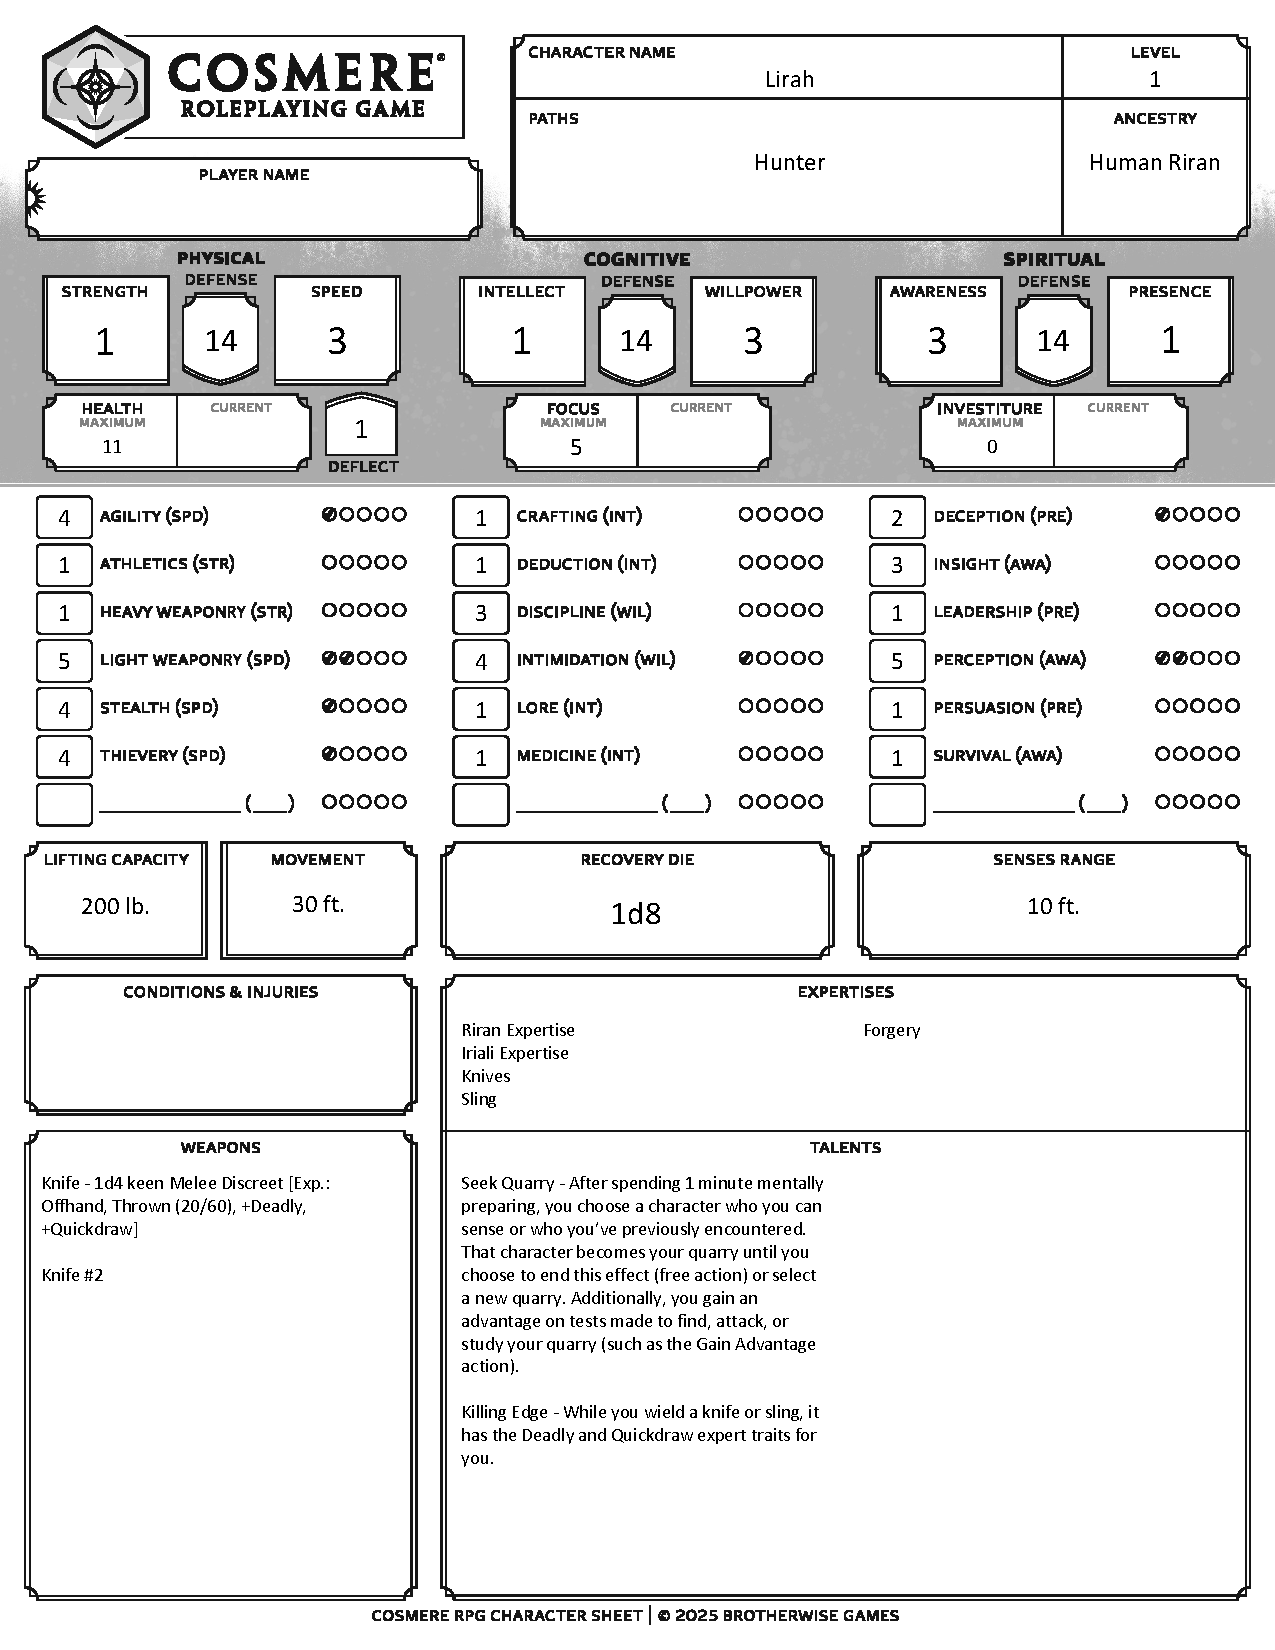
\includepdf[pages=-]{appendices/exampleSheets/example_sheet_riran_hunter_print.pdf}
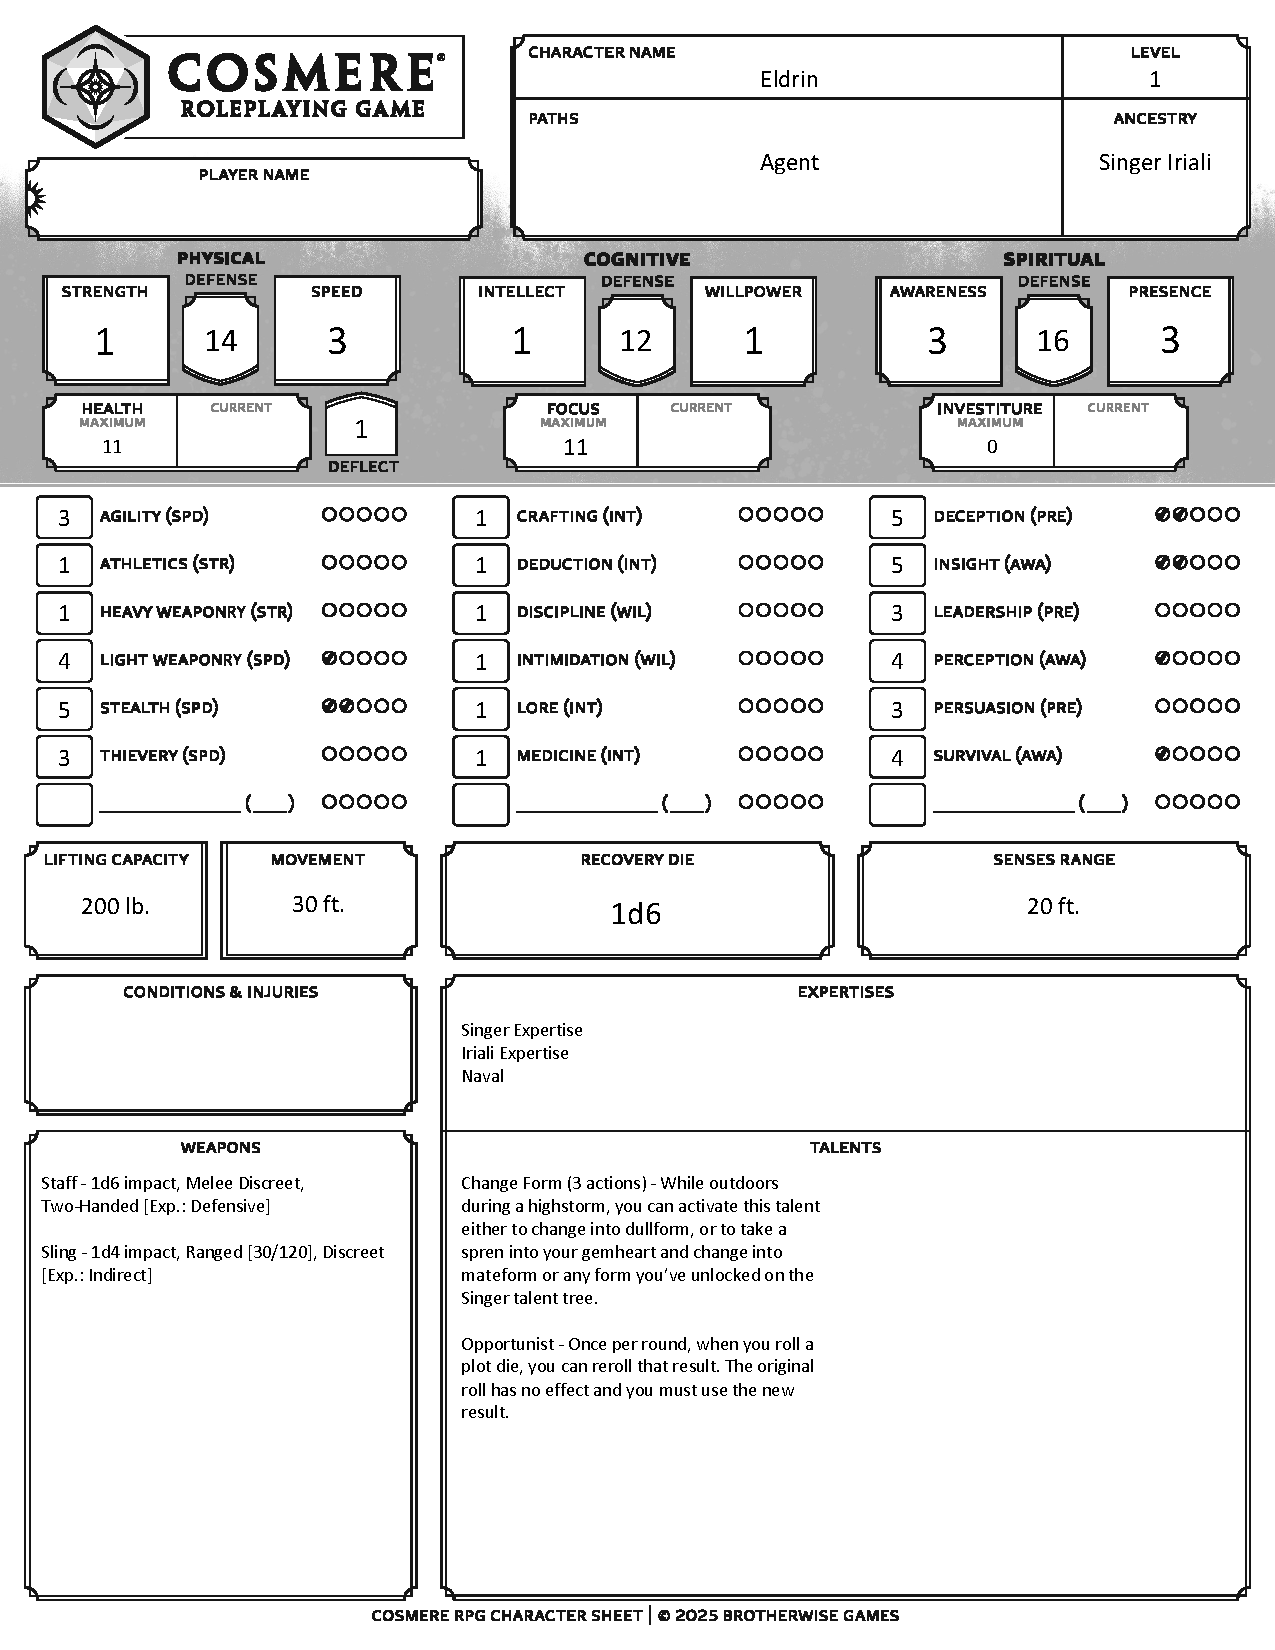
\includepdf[pages=-]{appendices/exampleSheets/example_sheet_singer_agent_print.pdf}


	\chapter{Appendix \thechapter{}: Example Maps}
\label{chap:exampleMaps}

Here are some example maps you can use for this adventure. While browsing the .pdf file, right-click on one of them to copy it and save it in its full size. \\

\noindent\textbf{\Large Jungles of \theIsland{}} \\

\begin{figure}[h]
	\centering
	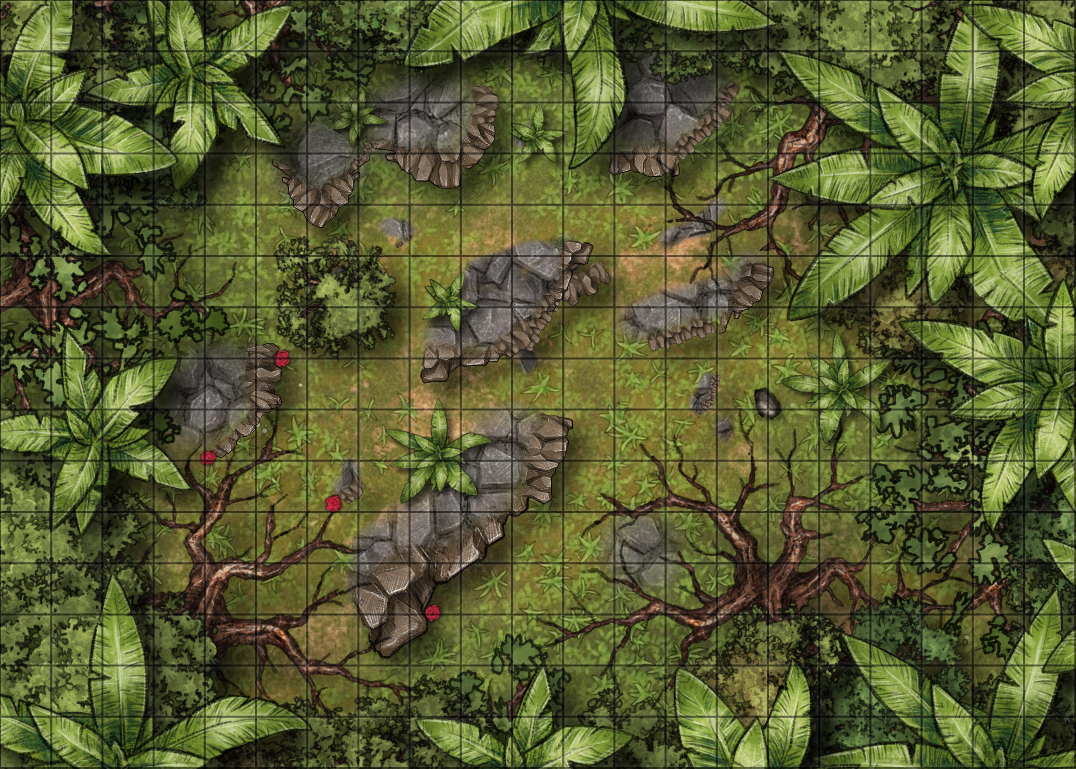
\includegraphics[width=0.45\textwidth]{maps/jungle.png}
	\caption{Jungles of \theIsland{}. }
	\label{fig:mapJungle}
\end{figure} 

\noindent\textbf{\Large Entrance to the temple} \\

\begin{figure}[h]
	\centering
	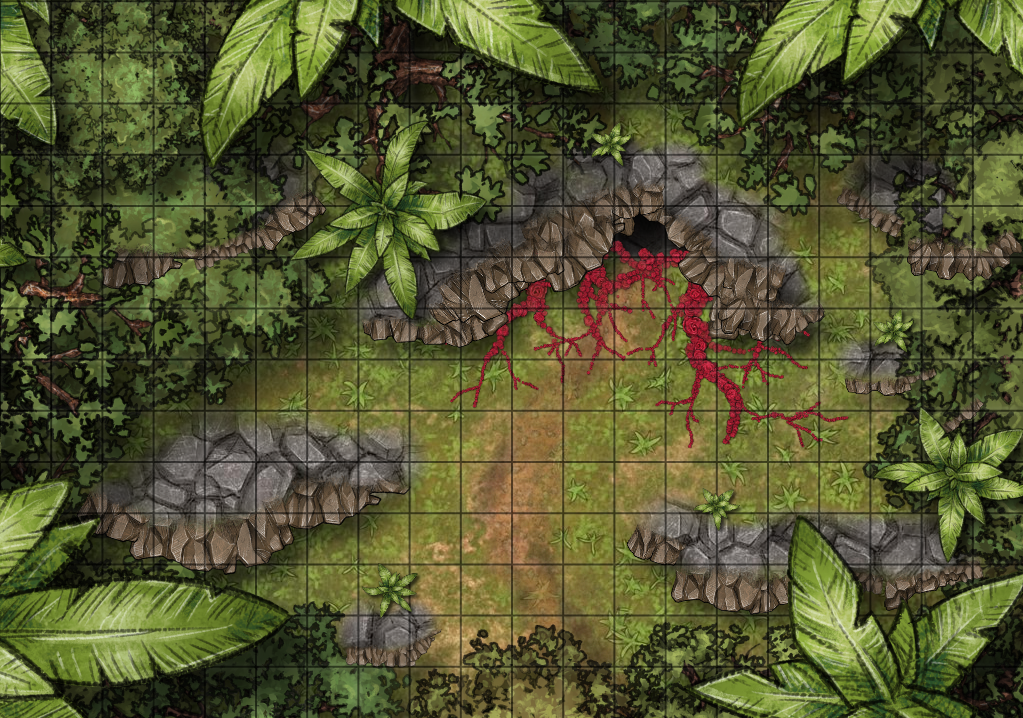
\includegraphics[width=0.45\textwidth]{maps/templeEntrance.png}
	\caption{Entrance to the temple of \npcSprenVines{}. }
	\label{fig:mapTempleEntrance}
\end{figure}

\newpage

\noindent\textbf{\Large Warehouse in Rall Elorim} \\

\begin{figure}[h]
	\centering
	\includegraphics[width=0.45\textwidth]{maps/warehouse.png}
	\caption{Warehouse in Rall Elorim. }
	\label{fig:mapWarehouse}
\end{figure}

\noindent\textbf{\Large Ancient Altar} \\

\begin{figure}[h]
	\centering
	\includegraphics[width=0.45\textwidth]{maps/altar.png}
	\caption{Ancient altar of \npcSprenVines{}. }
	\label{fig:mapAltar}
\end{figure}



	\chapter{Appendix \thechapter{}: Acknowledgments}
\label{chap:acknowledgments}

I poured my heart into this project, but I couldn't make it by myself alone. Here is quick thank you for all of those, who helped me do it, as well as a few other acknowledgments. \\ \\


\noindent\textbf{\Large My lovely wife} \\

My gemheart, moon of my life, the harbor of my soul’s journeying, thank you for all the help during this project! \\ \\


\noindent\textbf{\Large My fluffiest cat} \\

To Leo, the best, cutiest, fluffiest cat in the world! Thank you for your soothing purring, gentle rubs and musical meows to provide emotional support during all those evenings.

Thank you for reminding me that there is a time to write adventures, but also a time for a break, pets, belly rubs, fun and games!

Thank you for alerting me that the bowl is empty just in time to avert any disaster that could fall on our house for this transgression!

But on top of that, thank you for being so purrrfect! \\ \\


\noindent\textbf{\Large Anomer} \\

Anomer, my dear friend, thank you for all shared RPG discussions and your feedback on dungeon designing process.\\ \\


\newpage
\noindent\textbf{\Large Artists involved} \\

I cannot express my gratitude enough to all talented artists whose masterpieces show us the world of Roshar and its wonders. In particular I want to thank those, who created art for this book:

\begin{itemize}	
	\item Caio Santos \\
	\url{https://caiosantos.carrd.co/} \\
	\textit{Reanimated Whitespine}
\end{itemize}

If you are an artist and this book inspired you to create some epic illustration, please reach out! It would be great if I could include your art in here! \\ \\


\noindent\textbf{\Large Map generation} \\ 

Maps included in \nameref{chap:exampleMaps} were created with free trial version of Inkarnate. You can find this online tool in here: 

\url{https://inkarnate.com} \\ \\


\ifthenelse{\equal{\useAI}{false}}{}{
	\noindent\textbf{\Large Image generation} \\ 
	
	Images used in this book are generated by ChatGPT. Before you will have any ideas - I used this tool only for image generation, the story and other ideas are not AI-generated. \\ \\
}

\noindent\textbf{\Large PDF Building} \\ 

This document was written in TeXstudio with MiKTeX 24.1.


	
\end{document}